\documentclass[twoside,11pt,openright]{report}

\usepackage[utf8]{inputenc}
\usepackage[american]{babel}
\usepackage{a4}
\usepackage{latexsym}
\usepackage{amssymb}
\usepackage{amsmath}
\usepackage{epsfig}
\usepackage[T1]{fontenc}
\usepackage{mathptmx}
\usepackage{color}
\usepackage{epstopdf}
\usepackage{microtype}
\usepackage{hyperref}
\usepackage[useregional]{datetime2}
\DTMlangsetup[en-US]{showdayofmonth=false}
\usepackage{lipsum}
\usepackage{natbib}
\usepackage{graphicx}
\usepackage{caption}
\usepackage{url}
\usepackage{hyperref}
\usepackage{booktabs}
\usepackage{multirow}
\usepackage{makecell}
\usepackage{soul}
\usepackage{siunitx} 
\usepackage{booktabs}
\usepackage{multirow}
\usepackage{makecell}
\usepackage{float}
\raggedbottom

\renewcommand*\sfdefault{lmss}
\renewcommand*\ttdefault{txtt}

\newcommand{\todo}[1]{{\color[rgb]{.5,0,0}\textbf{$\blacktriangleright$#1$\blacktriangleleft$}}}

\begin{document}

%%%%%%%%%%%%%%%%%%%%%%%%%%%%%%%%%%%%%%%%%%%%%%%%%%%%%%%%%%%%%%%%%%%%%%%

\pagestyle{empty} 
\pagenumbering{roman} 
\vspace*{\fill}\noindent{\rule{\linewidth}{1mm}\\[4ex]
{\Huge\sf Efficient Time-Series Anomaly Detection for IoT Systems}\\[2ex]
{\huge\sf Fanni Ferenczi, 202402635}\\[2ex]
\noindent\rule{\linewidth}{1mm}\\[4ex]
\noindent{\Large\sf Master's Thesis, Computer Science\\[1ex] 
\today \\[1ex] Advisors: Qi Zhang, Gin\'es Carreto Pic\'on\\[15ex]}\\[\fill]}

\epsfig{file=logo.eps}\clearpage

%%%%%%%%%%%%%%%%%%%%%%%%%%%%%%%%%%%%%%%%%%%%%%%%%%%%%%%%%%%%%%%%%%%%%%%

\pagestyle{plain}
\chapter*{Abstract}
\addcontentsline{toc}{chapter}{Abstract}

Deep learning models for time series anomaly detection have achieved impressive
accuracy on benchmark datasets, yet their suitability for deployment on
resource-constrained IoT edge devices remains poorly understood. This thesis
addresses that gap by benchmarking five deep learning models --- TimesNet,
ModernTCN, TranAD, Anomaly Transformer, and GTA --- across two complementary
evaluation axes: detection accuracy and computational efficiency. Each model
represents a distinct architectural family, spanning convolutional,
transformer-based, and graph-based approaches. All five models are evaluated
on five widely adopted multivariate time series anomaly detection benchmarks
--- SMD, MSL, SMAP, SWaT, and PSM --- using point-adjusted F1 score and
AU-PR for accuracy, and MAC counts, memory footprint, and inference speed
for efficiency. Efficiency measurements are conducted on both a server-grade
GPU environment and a resource-constrained edge device, providing a direct
assessment of deployment feasibility under realistic hardware constraints.

The accuracy results show that Anomaly Transformer achieves the highest average
F1 score, while TranAD leads on AU-PR. Notably, the two
metrics do not always agree: a model can rank first on F1 while performing near
the bottom on AU-PR, which reflects the sensitivity of point-adjusted F1 to
threshold selection. Reporting both metrics together therefore provides a more
complete picture of detection quality than either metric alone.

On the efficiency side, the results demonstrate that architectural design choices
dominate deployment suitability more than any single metric in isolation. TranAD
emerges as the most memory-efficient and computationally cheapest model, achieving
competitive latency on both environments despite executing entirely on the CPU due
to a hardcoded implementation constraint. ModernTCN achieves the best latency and
throughput on both platforms and presents the most balanced overall profile.
Anomaly Transformer's runtime memory demand renders it infeasible on the edge
device at standard batch sizes. GTA, despite being designed explicitly for IoT
settings, incurs the highest edge latency of all five models.

The thesis concludes that no single model dominates across all dimensions
simultaneously. For deployments where memory is the binding constraint, TranAD
is the recommended choice. Where latency and throughput take priority, ModernTCN
offers the strongest overall profile.

\vspace{2ex}
\begin{flushright}
  \emph{Fanni Ferenczi,}\\
  \emph{Aarhus, \today.}
\end{flushright}

\tableofcontents
\cleardoublepage
\pagenumbering{arabic}
\setcounter{secnumdepth}{2}

%%%%%%%%%%%%%%%%%%%%%%%%%%%%%%%%%%%%%%%%%%%%%%%%%%%%%%%%%%%%%%%%%%%%%%%

\chapter{Introduction}
\label{ch:intro}

Time-series anomaly detection is critical for IoT systems, enabling predictive
maintenance, security monitoring, and system optimisation across a wide range of
cyber-physical applications. While recent deep learning
models achieve impressive accuracy on benchmark datasets, they face significant
challenges in real-world IoT deployments. Edge devices operate under strict resource
constraints --- limited computational power, memory, and energy --- and often require
low-latency responses. This creates a fundamental gap in
the existing literature: research predominantly optimises for detection accuracy,
while IoT deployments require balancing accuracy with practical constraints such as
computational efficiency, inference latency, and memory footprint.

This thesis addresses this gap by benchmarking five deep learning models for
multivariate time series anomaly detection with an explicit focus on their
suitability for IoT edge deployment. The five models --- TimesNet
\citep{timesnet2023}, ModernTCN \citep{moderntcn2024}, TranAD \citep{tranad2022},
Anomaly Transformer \citep{anomalytransformer2022}, and GTA \citep{gta2022} ---
were selected to represent a diverse range of architectures, spanning
convolutional, transformer-based, and graph-based approaches. Each model is
evaluated on five widely adopted benchmark datasets across two complementary axes:
detection accuracy, measured through point-adjusted F1 score and AU-PR, and
computational efficiency, characterised through MAC counts, memory footprint, and
inference speed measured on both a server-grade GPU environment and a
resource-constrained edge device. By examining how different model architectures
perform under IoT constraints, this work aims to develop insights into why certain
models are more suitable for constrained environments than others, and to provide
practical guidance for model selection in real-world deployment settings.

The thesis is structured as follows. Chapter~\ref{ch:intro} introduces the
problem of time series anomaly detection and the relevant background on deep
learning architectures and evaluation metrics. Chapter~2 describes the five
models evaluated in this thesis, covering their architectural design and anomaly
detection approach. Chapter~3 presents the experimental setup, datasets, and
results across both accuracy and efficiency dimensions. Chapter~4 concludes the
thesis with a summary of findings, a deployment recommendation, and directions
for future work.

\section{Anomalies in Time Series}
The detection of anomalies --- also referred to as outlier or novelty detection --- has been an active area of research across numerous application domains since the 1960s \citep{darban2024survey}.
With the growth of computational power and data availability, time series analysis has become increasingly central to addressing real-world problems through forecasting, classification, and anomaly detection.
Time Series Anomaly Detection (TSAD) has received growing attention due to its applicability across domains including urban management, intrusion detection, medical risk assessment, and natural disaster monitoring \citep{darban2024survey}.

\subsection{Time Series: Definitions and Types}
A \textbf{time series} is a series of data points indexed sequentially over time, with the most common form being a sequence of observations recorded at regular intervals \citep{darban2024survey}.
Time series are broadly divided into two types based on dimensionality.

\subsubsection{Univariate Time Series}
 
A univariate time series (UTS) consists of a single variable that changes over time.
Recording the humidity level every hour throughout a day is a typical example.
Formally, a UTS with $t$ timestamps is represented as an ordered sequence:
 
\begin{equation}
    \mathbf{X} = (x_1,\, x_2,\, \ldots,\, x_t)
    \label{eq:uts}
\end{equation}
 
\noindent where $x_i$ represents the observation at timestamp $i \in \mathcal{T}$ and $\mathcal{T} = \{1, 2, \ldots, t\}$ \citep{darban2024survey}.
 
\subsubsection{Multivariate Time Series}
 
A multivariate time series (MTS) represents multiple variables that simultaneously depend on time.
Each variable is influenced both by its own past values (\textit{temporal} dependency) and by other variables (\textit{spatial} or \textit{intermetric} dependency).
Formally, an MTS with $d$ dimensions over $t$ timestamps is represented as:
 
\begin{equation}
    \mathbf{X} = (X_1,\, X_2,\, \ldots,\, X_t), \quad
    X_i = \bigl(x_i^1,\, x_i^2,\, \ldots,\, x_i^d\bigr)
    \label{eq:mts}
\end{equation}
 
\noindent where $x_i^j$ denotes the observation of the $j$-th dimension at time $i$, and $d$ is the total number of dimensions \citep{darban2024survey}.


\subsection{Anomalies in Time Series}

An \textbf{anomaly} refers to a deviation from the general distribution of data --- either a single observation (\textit{point anomaly}) or a series of observations (\textit{subsequence anomaly}) that deviates significantly from the norm.
In real-world data, anomalies constitute only a small fraction of observations; the dataset mostly follows a normal pattern \citep{darban2024survey}.
 
Anomalies in time series can be classified as \textbf{temporal}, \textbf{intermetric}, or \textbf{temporal-intermetric} \citep{darban2024survey}, as illustrated in Figure~\ref{fig:anomaly_types}..

\begin{figure}[htbp]
    \centering
    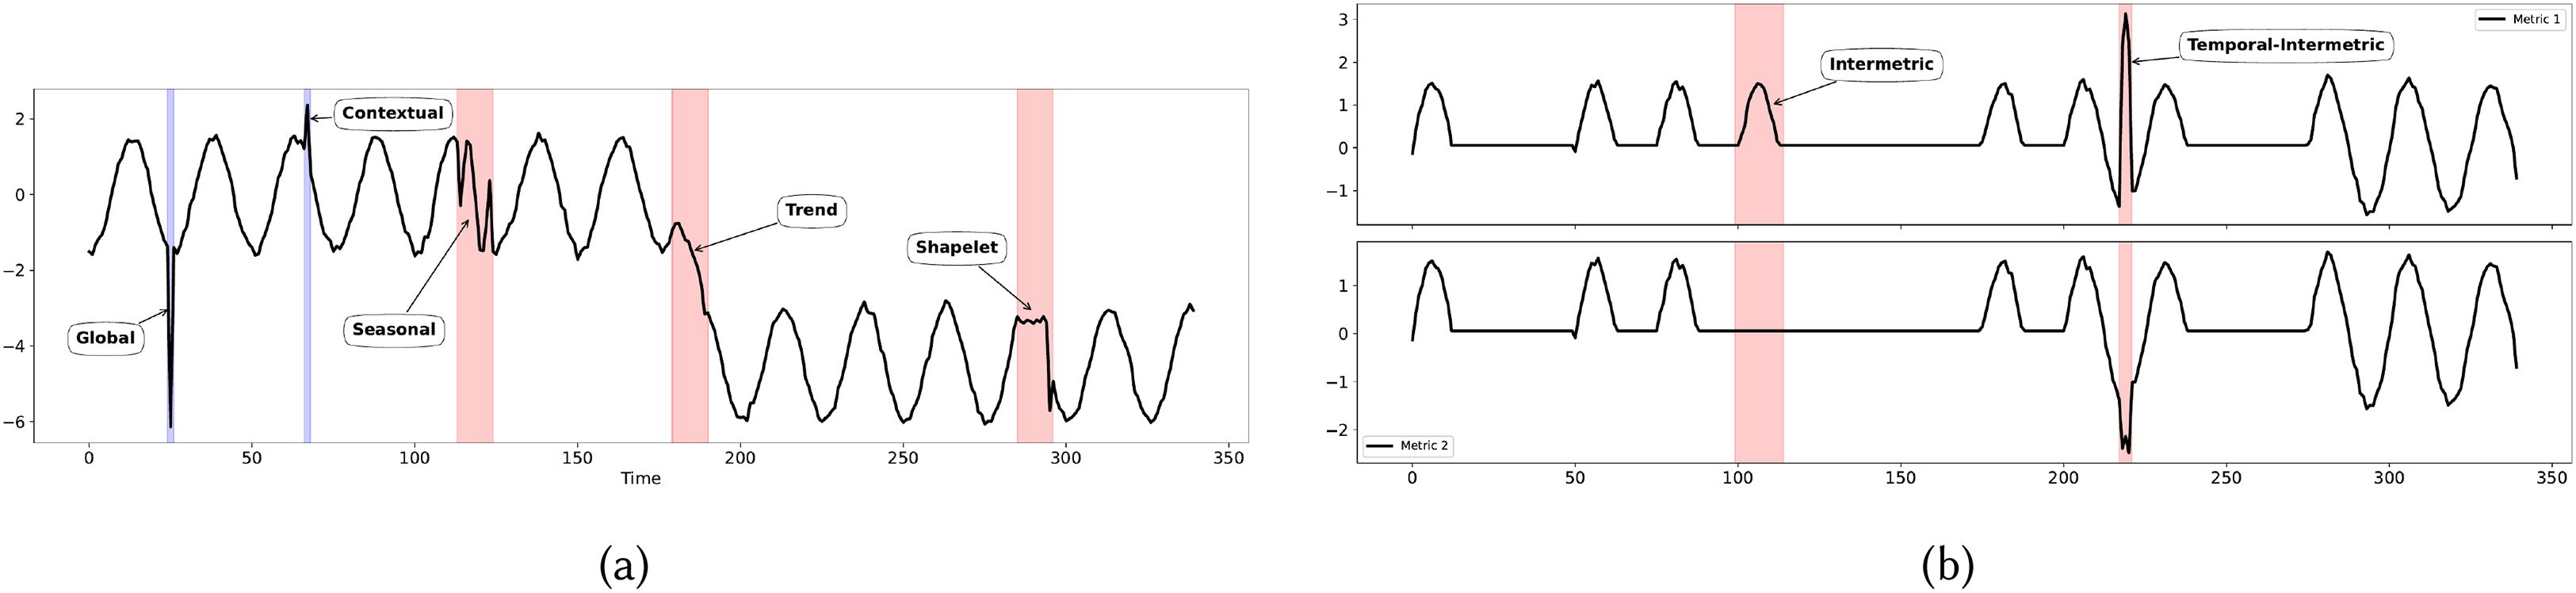
\includegraphics[width=\textwidth]{fig_anomaly_types.png}
    \caption{%
        Overview of anomaly types in time series.
        \textbf{(a)}~Temporal anomalies in a univariate time series (UTS): 
        global and contextual anomalies occur at individual points (blue), 
        while seasonal, trend, and shapelet anomalies span subsequences (red).
        \textbf{(b)}~Intermetric and temporal-intermetric anomalies in a 
        multivariate time series (MTS), where Metric~1 is power consumption 
        and Metric~2 is CPU usage.
        Figure extracted from \citep{darban2024survey}.%
    }
    \label{fig:anomaly_types}
\end{figure}
 
\subsubsection{Temporal Anomalies}
 
Temporal anomalies can be compared against neighbouring points (\textit{local}) or the entire series (\textit{global}), and they manifest in several distinct forms \citep{darban2024survey}:
 
\begin{itemize}
 
    \item \textbf{Global anomaly:}
    Spikes in the series where a point has an extreme value compared to the rest of the series (e.g., an unusually large payment on a typical day).
 
    \item \textbf{Contextual anomaly:}
    A deviation from a local neighbourhood --- a value that is normal in one context but anomalous in another (e.g., high transaction volume is normal on a public holiday but anomalous on a regular weekday).
 
    \item \textbf{Seasonal anomaly:}
    An unusual seasonality pattern despite otherwise normal shape and trend --- the frequency of rises and drops in a specific segment differs from the expected seasonal cycle.
 
    \item \textbf{Trend anomaly:}
    A permanent shift in the data's mean that alters the slope of the time series, while preserving its cycle and seasonality (e.g., a metric that rises abruptly and then drops following an external event).
 
    \item \textbf{Shapelet anomaly:}
    A subsequence whose shape or cycle pattern differs distinctly from the rest of the series (e.g., unusual economic fluctuation patterns due to demand-supply shocks).
 
\end{itemize}
 
\subsubsection{Intermetric Anomalies}

In an MTS, anomalies can also arise from a breakdown of spatial correlations between
dimensions. An \textbf{intermetric anomaly} occurs when the correlation between two or
more dimensions deteriorates within a time window, even though each individual dimension
appears normal in isolation \citep{darban2024survey}. As illustrated in
Figure~\ref{fig:anomaly_types}(b) (around $t \approx 100$), Metric~1 (power consumption)
and Metric~2 (CPU usage) are positively correlated under normal conditions --- both
signals follow a similar square-wave pattern. The intermetric anomaly (shaded in red)
marks the region where this correlation breaks down: Metric~1 exhibits an elevated spike
while Metric~2 remains flat, violating the expected joint behaviour despite neither
dimension being individually extreme.

\subsubsection{Temporal-Intermetric Anomalies}

\textbf{Temporal-intermetric anomalies} simultaneously violate both temporal patterns
and intermetric dependencies \citep{darban2024survey}. As shown in
Figure~\ref{fig:anomaly_types}(b) (around $t \approx 215$), the anomaly visible in
Metric~1 is not only a local spike that deviates from the expected temporal pattern of
that dimension, but also disrupts the correlation with Metric~2, which simultaneously
exhibits an inverted dip. This joint violation across time and dimensions makes
temporal-intermetric anomalies more complex to model, yet their multi-dimensional
footprint can also make them easier to detect than purely temporal or purely intermetric
anomalies \citep{darban2024survey}.

%%%%%%%%%%%%%%%%%%%%%%%%%%%

\section{Traditional Detection Methods}

Before the widespread adoption of deep learning, TSAD relied on several classical strategies \citep{darban2024survey}:
 
\begin{itemize}
    \item \textbf{Statistical methods:} Learn a statistical model of normal behaviour and flag deviations from it. These methods aim to model the normal 
    distribution of the time series and detect points that deviate significantly from the expected 
    distribution\citep{darban2024survey}.
    \item \textbf{Clustering-based methods:} Learn a normal profile of time series windows and 
    use the distance to the centroid of normal clusters as an anomaly score, or identify clusters 
    with few members as anomalous \citep{darban2024survey}. More recent methods in this 
    category first cluster the data to obtain a representation of normal behaviour and then compute 
    the distance to this normal behaviour to detect anomalies \citep{boniol2023trends}.
    \item \textbf{Distance-based methods:} Use the distance from a time window to its nearest 
    neighbours as an anomaly score \citep{darban2024survey}. A prominent example is 
    discord-based approaches, which identify subsequences that are maximally different from 
    all others in the time series using nearest-neighbour distances \citep{boniol2023trends}.
    \item \textbf{Density-based methods:} Estimate the local density of data points; windows 
    falling in low-density regions are flagged as anomalies \citep{darban2024survey}. Rather 
    than measuring nearest-neighbour distances, these methods focus on detecting globally 
    isolated behaviours. Isolation Forest \citep{liu2008isolation} is a notable example in this category, isolating 
    instances by building random splitting trees, where a shorter path length in the tree 
    indicates a higher likelihood of being anomalous \citep{boniol2023trends}.
\end{itemize}



%%%%%%%%%%%%%%%%%%%%%%%%%%%%%
\section{Deep Models for Time Series Anomaly Detection}

Deep learning has become increasingly capable of learning expressive representations of complex time series, including multidimensional data with both spatial (intermetric) and temporal characteristics.
In deep anomaly detection, neural networks are used to learn feature representations or anomaly scores in order to detect anomalies.
Many deep anomaly detection models have been developed, providing significantly higher performance than traditional TSAD methods across a wide range of real-world applications \citep{darban2024survey}.
A range of deep architectures has been explored for anomaly detection, including:
 
\begin{itemize}
    \item \textbf{Recurrent Neural Networks (RNN),} including Long Short-Term Memory (LSTM) 
    and Gated Recurrent Unit (GRU). RNNs have internal memory allowing them to process 
    variable-length input sequences and retain temporal dynamics \citep{darban2024survey}. 
    LSTM networks extend RNNs with memory lasting thousands of steps, enabling superior 
    modelling of long-term dependencies. Notable models in this category include LSTM-AD 
    \citep{malhotra2015lstm}, which uses hierarchical recurrent layers for unsupervised anomaly 
    detection in univariate time series, and LSTM-NDT \citep{hundman2018detecting}, which 
    combines LSTM with Nonparametric Dynamic Thresholding (NDT) \citep{hundman2018ndt}  for spacecraft anomaly detection. 
    GRU \citep{cho2014properties} offers a simpler gating structure than LSTM, leading to faster training times while 
    retaining the ability to capture temporal dependencies \citep{darban2024survey}.

    \item \textbf{Convolutional Neural Networks (CNN),} including Temporal Convolutional 
    Networks (TCN) \citep{bai2018empirical}. CNNs are adaptations of multilayer perceptrons designed to 
    identify hierarchical patterns in data. These
    networks employ convolutional, pooling, and fully connected layers, \citep{darban2024survey}. 
    DeepAnT \citep{munir2018deepant} is a notable CNN-based model that 
    efficiently detects small deviations in time series patterns with minimal training data.
    Despite their effectiveness, traditional CNNs struggle with sequential data due to their inherent
    design.
    TCNs address the 
    limitation of standard CNNs with sequential data by using dilated convolutions to 
    accommodate time series, ensuring that all computations for a timestamp use only 
    historical data \citep{darban2024survey}.
    TCN-ms \citep{he2019temporal} uses a TCN trained on normal data to forecast trends and 
    calculate anomaly scores using a multivariate Gaussian distribution fitted to prediction 
    errors, including a skipping connection to blend multi-scale features.

    \item \textbf{Autoencoders (AE)} \citep{kramer1991nonlinear}, including Sparse AE (SAE) \citep{ng2011sparse}, 
    Denoising AE (DAE) \citep{vincent2008extracting}, 
    Convolutional AE (CAE) \citep{noh2015learning}, and Variational AE (VAE) \citep{kingma2014auto}. 
    AEs consist of an encoder that 
    compresses input into a low-dimensional latent representation and a decoder that 
    reconstructs the input, with anomalies detected based on high reconstruction error 
    \citep{darban2024survey}. VAEs extend this framework by encoding inputs as 
    distributions rather than single points, enabling probabilistic anomaly scoring. 
    OmniAnomaly \citep{su2019robust} uses a VAE with stochastic RNNs for robust 
    representations of multivariate data and applies Peaks-Over-Threshold (POT) \citep{siffer2017pot} for thresholding. USAD 
    \citep{audibert2020usad} employs adversarially trained AEs to amplify reconstruction 
    errors and distinguish anomalies more reliably. RANSynCoders \citep{abdulaal2021practical} 
    proposes an architecture with multiple encoders and decoders using random feature 
    selection and majority voting to localise anomalies, developed for real-time use at eBay.

    \item \textbf{Generative Adversarial Networks (GAN).} GANs consist of a generator and 
    a discriminator trained adversarially, where the generator learns the normal data 
    distribution and the discriminator identifies deviations \citep{darban2024survey}. 
    MAD-GAN \citep{li2019madgan} uses LSTM-RNN as both generator and discriminator to 
    capture temporal relationships in multivariate time series, detecting anomalies via 
    reconstruction error and discrimination loss. BeatGAN \citep{zhou2019beatgan} combines 
    AEs and GANs to regularise reconstruction robustly, showing strong results on both ECG 
    and sensor data.

    \item \textbf{Graph Neural Networks (GNN),} including Graph Convolutional Networks 
    (GCN) \citep{kipf2017semi} and Graph Attention Networks (GAT) \citep{velickovic2018graph}. 
    GNNs extract spatial information from 
    multivariate time series by forming a graph structure in which each dimension is 
    represented as a node and edges indicate learned inter-sensor correlations 
    \citep{darban2024survey}. GDN \citep{deng2021graph} is a GNN attention-based model 
    that captures sensor characteristics as nodes and their correlations as edges, predicting 
    behaviour based on adjacent sensors. 

    \item \textbf{Transformers.} Transformers \citep{vaswani2017attention} process the entire input sequence simultaneously 
    using attention mechanisms, enabling efficient capture of long-term dependencies without 
    recurrence \citep{darban2024survey}. Anomaly Transformer \citep{anomalytransformer2022} 
    introduces an association discrepancy criterion that simultaneously models prior and 
    series associations for each timestamp, making rare anomalies more distinguishable. 
    TranAD \citep{tranad2022} adds self-conditioning and adversarial training to a 
    transformer-based architecture, amplifying subtle reconstruction errors and improving 
    generalisation on large multivariate inputs.

    \item \textbf{Hierarchical Temporal Memory (HTM).} HTM \citep{george2008brain} mimics the hierarchical 
    processing of the neocortex, encoding inputs through sparse spatial pooling and 
    modelling temporal patterns via sequence memory \citep{darban2024survey}. It is robust 
    to noise, has high capacity, and can learn multiple patterns simultaneously. Numenta HTM 
    \citep{ahmad2017unsupervised} detects temporal anomalies in univariate time series in 
    both predictable and noisy environments, adapting continuously to changes without 
    requiring labelled data.
\end{itemize}
 
Deep TSAD models process inputs either point-by-point or using sliding windows, and output either continuous anomaly scores or binary labels \citep{darban2024survey}.
Common thresholding methods applied to anomaly scores include NDT \citep{hundman2018ndt} and POT \citep{siffer2017pot}.
 
\subsubsection{Learning Schemes}
 
Deep TSAD models operate under four learning paradigms \citep{darban2024survey}:
 
\begin{itemize}
    \item \textbf{Unsupervised:} No labels are used; anomaly detection relies solely on intrinsic features of the data. This is the most flexible scheme and is suitable for streaming applications, though evaluation is more challenging.
    \item \textbf{Semi-supervised:} Trained exclusively on labelled \textit{normal} data; deviations from the learned normal distribution are flagged as anomalies.
    \item \textbf{Supervised:} Uses a fully labelled dataset containing both normal and anomalous examples. It can produce appropriate threshold value, but impractical in many real-world settings where anomalies are unlabelled.
    \item \textbf{Self-supervised:} The model generates its own supervisory signal from the input data without explicit labels, typically via contrastive learning or data augmentation strategies.
\end{itemize}
 
% ------------------------------------------------------------
\subsection{Deep Learning Approaches in TSAD}
\label{sec:dl_approaches}
% ------------------------------------------------------------
 
The deep learning literature on TSAD is commonly structured around four
main detection approaches: \textbf{forecasting-based},
\textbf{reconstruction-based}, \textbf{representation-based}, and
\textbf{hybrid} \citep{darban2024survey}.
 
\subsubsection{Forecasting-Based Approach}
\label{sec:forecasting_based}
 
Forecasting-based models learn to predict future values of a time series and use the prediction error as an anomaly score:
the larger the deviation between the predicted and actual value, the more anomalous the observation is considered.
Most forecasting methods employ a sliding window to forecast one point at a time \citep{darban2024survey}.
 
This approach performs well when normal behaviour is abundant and anomalous behaviour is rare.
However, it struggles with rapidly changing time series where future states are fundamentally unpredictable \citep{darban2024survey}.
 
 
\subsubsection{Reconstruction-Based Approach}
\label{sec:reconstruction_based}
 
Reconstruction-based models encode subsequences of normal training data into a low-dimensional latent space and then reconstruct them.
The underlying hypothesis is that anomalous subsequences --- which are unseen during training --- will be reconstructed with higher error than normal patterns.
This reconstruction error constitutes the anomaly score \citep{darban2024survey}.
 
Unlike forecasting-based models, reconstruction-based models have access to the \textit{current} time series window, enabling more accurate detection.
They are preferred when high accuracy is paramount and some detection delay is acceptable \citep{darban2024survey}.
 
\subsubsection{Representation-Based Approach}
\label{sec:representation_based}
 
Representation-based models focus on learning rich, generalisable latent representations of time series that can subsequently be used for anomaly detection as a downstream task.
Rather than operating in raw input space, anomaly detection is performed in the learned latent space.
These models are particularly useful when labelled data is scarce, as they commonly operate under unsupervised or self-supervised learning schemes.  \citep{darban2024survey}.
 
\subsubsection{Hybrid Approach}
\label{sec:hybrid}
 
Hybrid models integrate the strengths of multiple approaches --- for example, combining forecasting and reconstruction objectives within a single joint optimisation framework.
This allows the model to simultaneously benefit from prediction accuracy and latent space regularity \citep{darban2024survey}.

\section{Evaluation Metrics}
\label{sec:eval_metrics}
This section introduces the metrics used to evaluate model performance throughout 
this thesis. Evaluation is conducted along two complementary axes: detection 
accuracy, which measures how well each model identifies anomalous time steps, and 
computational efficiency, which assesses the practical suitability of each model 
for deployment on resource-constrained IoT edge devices.

\subsection{Accuracy}

Anomaly detection is fundamentally a binary classification problem: each time step is assigned
either a normal or an anomalous label. Evaluating this classification accurately is non-trivial
in the TSAD setting, where anomalies are rare by definition and the class distribution is
heavily imbalanced \cite{darban2024survey}. Four point-wise metrics are used throughout
this thesis to assess detection performance: Precision, Recall, F1 Score, and the Area Under
the Receiver Operating Characteristic Curve (AUC-ROC). These metrics are defined in terms
of the standard confusion matrix quantities: True Positives (\(\mathrm{TP}\)), False Positives
(\(\mathrm{FP}\)), True Negatives (\(\mathrm{TN}\)), and False Negatives (\(\mathrm{FN}\)).

\paragraph{Precision.}
Precision measures the proportion of time steps flagged as anomalous by the model that are
truly anomalous \cite{darban2024survey}. A low precision indicates that the model
generates many false alarms, incorrectly labelling normal behaviour as anomalous.

\begin{equation}
    \mathrm{Precision} = \frac{\mathrm{TP}}{\mathrm{TP} + \mathrm{FP}}
\end{equation}

\paragraph{Recall.}
Recall measures the proportion of actual anomalous time steps that the model successfully
detects \cite{darban2024survey}. A low recall indicates that many true anomalies are
missed.

\begin{equation}
    \mathrm{Recall} = \frac{\mathrm{TP}}{\mathrm{TP} + \mathrm{FN}}
\end{equation}

\paragraph{F1 Score.}
Precision and Recall are in tension: a model can trivially achieve perfect recall by flagging
every time step as anomalous, or perfect precision by only flagging the single most certain
anomaly. The F1 Score is the harmonic mean of the two, providing a single balanced measure
of detection quality \cite{darban2024survey}.

\begin{equation}
    \mathrm{F1} = 2 \cdot \frac{\mathrm{Precision} \cdot \mathrm{Recall}}{\mathrm{Precision} + \mathrm{Recall}}
\end{equation}

\noindent In this thesis, F1 scores are computed using the \emph{point adjustment} (PA)
protocol \cite{xu2018donut}. Under this convention, if at least one point within a contiguous
anomalous segment is detected by the model, all points in that segment are considered
correctly detected. This corresponds to an \emph{abnormal event detection} perspective: once
any part of an anomalous event is flagged, the entire event is considered found, which is
meaningful in real-world monitoring scenarios where a single alert would trigger a human
inspection of the surrounding time window \cite{xu2022detectionadjustment}.

Point adjustment is a widely adopted convention in the TSAD literature, and all baseline
results compared in this thesis are also evaluated under the same protocol
\cite{xu2022detectionadjustment}. This ensures a fair comparison across
models. It should nevertheless be noted that point adjustment can overestimate model
performance, particularly on datasets with long anomalous segments, since detecting even
a single point in a long segment credits the model with detecting the entire segment
\cite{darban2024carla}. The AU-PR metric described below is reported without point
adjustment and therefore provides a complementary, stricter perspective on model
performance.

\paragraph{Area Under the Precision-Recall Curve (AU-PR).}
The metrics above depend on a fixed anomaly threshold. In practice, anomaly scores are
continuous, and the choice of threshold is dataset- and application-specific. The Area Under
the Precision-Recall Curve (AU-PR) provides a threshold-independent summary of model
performance \cite{darban2024survey}:
\begin{equation}
    \mathrm{AU\text{-}PR} = \int_{0}^{1} \mathrm{Precision}(t)\,
    \frac{d(\mathrm{Recall}(t))}{dt}\, dt
\end{equation}

\noindent AU-PR is particularly suited to heavily imbalanced datasets, where anomalies
constitute only a small fraction of all observations \cite{darban2024survey}. Unlike
AUC-ROC, which weights true positive and false positive rates symmetrically regardless of
class frequency, AU-PR focuses directly on the model's ability to retrieve the rare anomalous
class with high precision. Because it is computed from raw anomaly scores without applying
point adjustment, it also serves as a more conservative measure of performance than the
point-adjusted F1 score, and is therefore useful for cross-model comparison that is not
subject to the inflation effects of the PA protocol.



\subsection{Number of operations}
\label{subsec:macs}

Measuring the computational cost of a model is essential for evaluating its suitability
for deployment on resource-constrained IoT edge devices. Unlike wall-clock latency,
which is sensitive to hardware, software stack, and execution environment, the number
of arithmetic operations performed during a forward pass provides a hardware-independent
characterisation of computational complexity that can be compared across models and
platforms.

\paragraph{Multiply-Accumulate Operations (MACs).}
The standard unit used to quantify the computational cost of deep learning inference
is the \emph{Multiply-Accumulate operation} (MAC). A single MAC corresponds to one
multiplication followed by one addition, the elementary operation in dot products,
convolutions, and matrix multiplications that constitute the bulk of deep neural
network computation. Because one MAC equals two floating-point operations (FLOPs),
the two units are often used interchangeably in the literature, with the relationship
$\mathrm{FLOPs} \approx 2 \times \mathrm{MACs}$.

For edge deployment, the MAC count of a model's forward pass is a primary indicator
of whether it can meet real-time latency budgets on hardware with limited floating-point
throughput, such as microcontrollers or low-power embedded processors. A lower MAC
count generally implies lower energy consumption, lower heat dissipation, and the
possibility of deployment on cheaper or more constrained hardware.

\paragraph{Measurement with \texttt{fvcore}.}
All MAC counts reported in this thesis are measured using \texttt{fvcore} \cite{fvcore}, an open-source
library developed by Meta Research that provides a \texttt{FlopCountAnalysis} utility for
PyTorch models. \texttt{fvcore} works by tracing the model's computational graph on a
given input tensor and registering a hook for each operator encountered. For each
registered operator — such as \texttt{nn.Linear} or \texttt{nn.Conv1d} — a handler function computes the theoretical MAC count from the
operator's input and output shapes. The total MAC count is then the sum of all
per-operator counts accumulated over a single forward pass.

\paragraph{Coverage gaps and custom handlers.}
\texttt{fvcore} provides built-in handlers for the most common PyTorch operators,
particularly those dominated by matrix multiplication, such as linear projections and
convolutions. However, it does not cover all operations present in every architecture.
Specifically, element-wise operations such as softmax, layer normalisation, residual
additions, and activation functions are not counted by default, as \texttt{fvcore}
registers them as unsupported and silently omits their contribution.

For convolution-based models such as TimesNet \cite{timesnet2023} and ModernTCN
\cite{moderntcn2024}, the built-in handlers provided sufficient coverage, since the
dominant cost lies in convolutional and linear layers that \texttt{fvcore} handles
natively. For the Transformer-based models evaluated in this thesis --- TranAD
\cite{tranad2022}, Anomaly Transformer \cite{anomalytransformer2022}, and GTA
\cite{gta2022} --- the standard handlers were insufficient. \texttt{fvcore} only
registers handlers for a subset of PyTorch operators, and silently omits any operation
for which no handler is defined. For these architectures, a range of operations went
uncounted by default, including element-wise arithmetic (e.g.\ \texttt{aten::mul}), 
activation functions (e.g.\ \texttt{aten::softmax}), and other operations such as
\texttt{aten::pow}. Custom operator handlers were therefore
implemented and registered with \texttt{fvcore}'s analysis object to cover these
missing operations. The reported MAC counts should consequently be
interpreted as lower bounds on the true per-forward-pass cost, suitable for relative
cross-model comparison rather than absolute throughput estimation.

\subsection{Memory Usage}
\label{subsec:memory}

Memory footprint is a critical constraint for IoT edge deployment, where devices
operate under strict memory budgets. Five memory-related metrics are reported for each model in this thesis,
each capturing a different aspect of the model's memory demand. One model requires special 
treatment throughout: TranAD's original codebase hardcodes execution to the CPU via explicit 
\texttt{.cpu()} calls \citep{tranad2022}, meaning all its memory figures are measured from 
CPU RAM rather than GPU VRAM.

\paragraph{Parameter count.}
The parameter count is the total number of individually learnable scalar values in
the model --- all weights and biases across every layer. This number determines the
minimum information that must be stored to represent a trained model, and is a
hardware-independent measure of model size. A model with fewer parameters is
generally cheaper to store and transfer, and is more likely to fit within the flash
or RAM constraints of an edge device.

\paragraph{Weight memory (exact).}
The exact weight memory is the parameter count multiplied by the number of bytes per
value, and is hardware-independent. For TimesNet, ModernTCN, and Anomaly Transformer, 
which operate in \texttt{float32}, this equals $\mathrm{Params} \times 4\ \mathrm{bytes}$. 
TranAD and GTA both operate in \texttt{float64} at runtime, so their exact weight memory is computed as 
$\mathrm{Params} \times 8\ \mathrm{bytes}$. This represents the minimum memory required 
to hold the trained model and is the most direct measure of storage cost for deployment.

\paragraph{Weight memory (allocated).}
The allocated weight memory is the amount of memory the runtime actually
reserves for the model's parameters, as reported by PyTorch's memory allocator. This
value can exceed the exact weight memory because PyTorch allocates memory in blocks
and may also include persistent buffers that are part of the model's state but are not updated by
gradient descent. For TimesNet, ModernTCN, Anomaly Transformer, and GTA 
this is measured from GPU VRAM via PyTorch's GPU memory tracker. For TranAD, it is 
measured from CPU RAM via the CPU memory allocator.

\paragraph{Peak training memory.}
The peak training memory is the maximum GPU memory occupied at any point during a
training forward-backward pass. It is substantially larger than the inference memory
because during backpropagation PyTorch must retain all intermediate activations
produced during the forward pass in order to compute gradients.
For all models except TranAD, this is measured in GPU VRAM. For TranAD, it is measured 
in CPU RAM, reflecting its CPU-only execution.

\paragraph{Peak inference memory.}
The peak inference memory is the maximum GPU memory occupied during a forward pass
on the test set, with no gradient computation. This is the relevant memory figure
for deployment, since in production the model only performs forward passes on new
incoming data. During training, PyTorch builds a 
computational graph by retaining all intermediate activation tensors --- that is, the 
output of every layer --- rather than discarding them after use \citep{pytorch_autograd}. This is necessary because 
the backward pass computes gradients via the chain rule, and each layer's gradient depends 
on the activations produced by that layer during the forward pass. At inference time, 
however, no such graph is needed: activations can be discarded immediately after each 
layer has produced its output, which is why peak inference memory is substantially lower 
than peak training memory. As with peak training 
memory, this figure is measured in GPU VRAM for all models except TranAD, for which it 
reflects CPU RAM.

\paragraph{Memory overhead.}
The memory overhead is defined as the difference between the peak training memory
and the exact weight memory:
\begin{equation}
    \mathrm{Overhead} = \mathrm{Peak\ training\ memory} - \mathrm{Weight\ memory\ (exact)}
\end{equation}
It quantifies everything that is not the model weights themselves: temporary tensors,
intermediate activations, gradient buffers, and other bookkeeping structures that
PyTorch allocates during a training step. A large overhead relative to the weight
memory indicates that the model's training cost is dominated by the computation graph
rather than by the number of parameters. For TranAD, the overhead is computed from 
CPU RAM measurements and should be interpreted accordingly.


\subsection{Inference Speed}

Beyond memory and computational cost, the time a model takes to process incoming
data is a critical constraint for edge deployment. Two complementary metrics are used to
characterise inference speed in this thesis.

\paragraph{Latency.}
Latency is defined here as the mean wall-clock time required to process one batch
of input windows, measured in milliseconds. A batch consists of multiple fixed-length time-series windows. 
Latency captures the end-to-end delay from
receiving a batch of windows to producing anomaly scores for all windows in that batch 
and is therefore the most
directly relevant metric for assessing whether a model can operate within the
response time budget of a target application. A model with high latency may
produce accurate results but still be unsuitable for deployment in scenarios where
anomalies must be flagged within a tight time window.

\paragraph{Throughput.}
Throughput is defined as the number of input windows processed per second.
It is the inverse perspective of latency: where latency characterises the delay
for a single batch, throughput characterises how much data the model can handle
over time. In other words, throughput measures how many complete time-series windows 
the model can process per second under a fixed batch size.
Throughput is particularly relevant when evaluating a model's ability
to keep pace with the data rate of a sensor stream without accumulating a
backlog. 

\chapter{Chosen Models}

The five models evaluated in this thesis --- TimesNet \citep{timesnet2023} , ModernTCN \citep{moderntcn2024} , TranAD \citep{tranad2022}, 
Anomaly Transformer \citep{anomalytransformer2022} , and GTA \citep{gta2022} 
--- were selected to represent a diverse set of deep learning 
architectures for time series anomaly detection, spanning convolutional, transformer-based, 
and graph-based approaches. The selection was driven by a combination of reported accuracy, 
architectural diversity, and relevance to IoT edge deployment.

TimesNet \citep{timesnet2023} and ModernTCN \citep{moderntcn2024} were chosen as 
representatives of the CNN-based family. Both are task-general backbones that have 
demonstrated strong performance on anomaly detection benchmarks, and they are frequently 
compared against each other in the literature --- including directly in the ModernTCN 
paper itself \citep{moderntcn2024}. Their shared reconstruction-based detection strategy 
and similar evaluation setup make them a natural pair for cross-architectural comparison, 
while their different internal designs --- TimesNet's 2D transformation versus ModernTCN's 
large-kernel depthwise convolution --- make the comparison informative about what drives 
CNN performance in TSAD.

TranAD \citep{tranad2022} was selected as a representative of the Transformer-based
family, providing an architectural contrast to the two CNN-based models. Beyond
detection accuracy, TranAD was included for its efficiency-oriented design: its
compact encoder-decoder architecture make it a promising
candidate for resource-constrained edge deployment.

Anomaly Transformer \citep{anomalytransformer2022} was selected because it shows 
higher detection accuracy than TranAD across several benchmarks, making it a 
natural next candidate within the Transformer family. Its association discrepancy 
criterion --- which measures how a time point's attention distributes across the series 
rather than how poorly it is reconstructed --- represents a fundamentally different 
detection philosophy from TranAD's adversarial reconstruction amplification, making the 
comparison between the two architecturally and methodologically interesting.

GTA \citep{gta2022} is a model designed for IoT sensor 
data, which is directly relevant to the edge deployment focus of this thesis. Its 
graph-based architecture learns the dependency structure between sensors end-to-end, 
making it the only model in the evaluation set to explicitly model inter-sensor 
relationships as a graph topology. Combined with its forecasting-based detection 
approach --- which contrasts with the reconstruction-based strategy of all other 
selected models --- GTA broadens the architectural diversity of the evaluation and 
provides a perspective on how IoT-native design choices affect detection performance 
and efficiency.

\section{TimesNet}
TimesNet \citep{timesnet2023} is a task-general deep learning backbone for time series
analysis. Rather than targeting a single task, TimesNet is designed to perform competitively across five mainstream time
series analysis tasks simultaneously: short- and long-term forecasting, imputation,
classification, and anomaly detection \citep{timesnet2023}. In the context of this
thesis, it is evaluated strictly as an anomaly detection model.

\subsection{Multi-Periodicity and 2D Variation Modelling}

The central observation motivating TimesNet is that real-world time series
exhibit \textbf{multi-periodicity} --- for instance, daily and yearly variations in
weather data, or weekly and quarterly cycles in electricity consumption
\citep{timesnet2023}. Within each period, two distinct types of temporal variation
coexist:

\begin{itemize}
    \item \textbf{Intraperiod-variation}: short-term temporal patterns within a
    single period (captured along columns of a reshaped 2D tensor);
    \item \textbf{Interperiod-variation}: long-term trends across consecutive
    periods (captured along rows of the reshaped 2D tensor).
\end{itemize}

\noindent The key insight is that a 1D time series cannot explicitly represent both
variation types simultaneously. TimesNet addresses this by transforming the 1D
series into a set of 2D tensors --- one per dominant period --- allowing both
variation types to be modelled jointly using 2D convolutional kernels
\citep{timesnet2023}.

\subsection{Architecture}
The overall architecture of TimesNet consists of $N$ stacked \textbf{TimesBlocks}
connected residually, as shown in Figure~\ref{fig:timesnet_architecture}. Each
TimesBlock transforms its 1D input representation and returns an enriched 1D
output of the same length, which is passed to the next block. The full processing
pipeline within a single TimesBlock proceeds in three conceptual stages
\citep{timesnet2023}:

\begin{figure}[htbp]
    \centering
    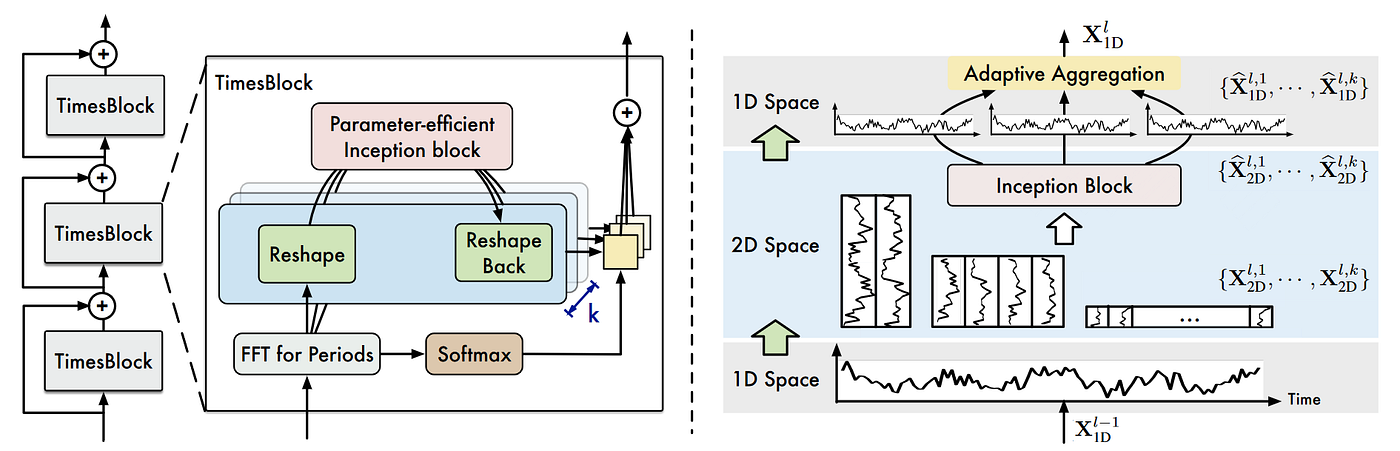
\includegraphics[width=\textwidth]{timesnet2.png}
    \caption{Overall architecture of TimesNet (left) and the internal data flow
    of a single TimesBlock (right). The 1D input is first transformed into $k$
    structured 2D tensors via FFT-based period discovery and reshaping. Each
    tensor is processed by a shared parameter-efficient inception block in 2D
    space. The resulting representations are projected back to 1D and fused
    via amplitude-weighted adaptive aggregation to produce the output.
    Figure extracted from \citep{timesnet2023}.}
    \label{fig:timesnet_architecture}
\end{figure}

\paragraph{Period discovery.}
The dominant periodicities of the input signal are identified automatically using
Fast Fourier Transform (FFT). The top-$k$ frequencies by spectral amplitude are
selected, each corresponding to a distinct period length. This step is fully
data-driven and requires no prior domain knowledge about the periodicity structure
of the time series \citep{timesnet2023}.

\paragraph{1D-to-2D transformation and representation learning.}
For each of the $k$ discovered periods, the 1D input is reshaped into a 2D tensor,
where columns correspond to within-period time points (intraperiod-variation) and
rows correspond to the same phase across successive periods (interperiod-variation).
Each 2D tensor is then processed by a \textbf{shared parameter-efficient inception
block} \citep{szegedy2015inception}, which applies multi-scale 2D convolutional
kernels to capture both variation types jointly. Because the same inception block
is shared across all $k$ tensors, the total number of model parameters remains
constant regardless of how many periods are selected --- a property that is
particularly relevant for deployment in resource-constrained environments
\citep{timesnet2023}.

\paragraph{Adaptive aggregation.}
The $k$ processed 2D representations are projected back to 1D space and fused into
a single output using the FFT spectral amplitudes as importance weights. Periods
with stronger spectral amplitude contribute more to the final representation,
ensuring that dominant periodicities have greater influence on the output
\citep{timesnet2023}.

\subsection{Anomaly Detection Approach}

TimesNet applies a \textbf{reconstruction-based} anomaly detection strategy. During
training on normal data, the model learns to reconstruct input windows with low
error. At inference time, anomalies are identified as time points whose
reconstruction error exceeds a threshold. 



\section{ModernTCN}

ModernTCN \citep{moderntcn2024} is a pure convolution-based backbone for general
time series analysis. Like
TimesNet, it targets five mainstream time series analysis tasks simultaneously (
short- and long-term forecasting, imputation, classification, and anomaly detection) but takes a
fundamentally different approach: rather than transforming the time series into 2D
space, ModernTCN instead modernises the convolution operation itself
\citep{moderntcn2024}. In the context of this thesis, it is evaluated strictly as an
anomaly detection model.

\subsection{Bringing Convolution Back}

The central argument of ModernTCN is that convolution-based models fell behind
Transformer-based models not because convolution is inherently limited, but because
previous convolution designs had a too-small \textbf{Effective Receptive Field (ERF)}
--- that is, they could only see a narrow window of the input at a time, making it
difficult to capture long-term temporal dependencies \citep{moderntcn2024}. Meanwhile,
Transformers with their global attention mechanism can in principle attend to any
part of the sequence, which is why they outperformed traditional temporal convolutional
networks (TCNs).

ModernTCN addresses this by drawing inspiration from recent advances in computer vision,
where modern convolution designs \citep{liu2022convnext} have shown that a redesigned
convolution block --- borrowing structural ideas from Transformers and using much larger
kernel sizes --- can match or exceed Transformer performance while retaining the speed
and memory efficiency of convolution \citep{moderntcn2024}. The key insight is that
enlarging the kernel size is a far more effective way to grow the receptive field than
stacking many small-kernel layers, as the ERF grows linearly with kernel size but only
sub-linearly with depth \citep{moderntcn2024}.

\subsection{Architecture}

The overall architecture of ModernTCN follows the same residual stacking pattern as
TimesNet: a series of \textbf{ModernTCN blocks} connected residually, preceded by a
patch embedding layer that converts the raw input into a sequence of fixed-size patch
tokens. Unlike many Transformer-based models that collapse all variables into a single
embedding, ModernTCN embeds each variable \textit{independently}, explicitly preserving
the variable dimension throughout the network so that both temporal and cross-variable
dependencies can be modelled separately and explicitly \citep{moderntcn2024}.

Each ModernTCN block, illustrated in Figure~\ref{fig:moderntcn_block}(d), is structured
similarly to a Transformer block but implemented entirely with convolutions. It contains
three components that each handle a distinct type of information mixing
\citep{moderntcn2024}:

\begin{figure}[htbp]
    \centering
    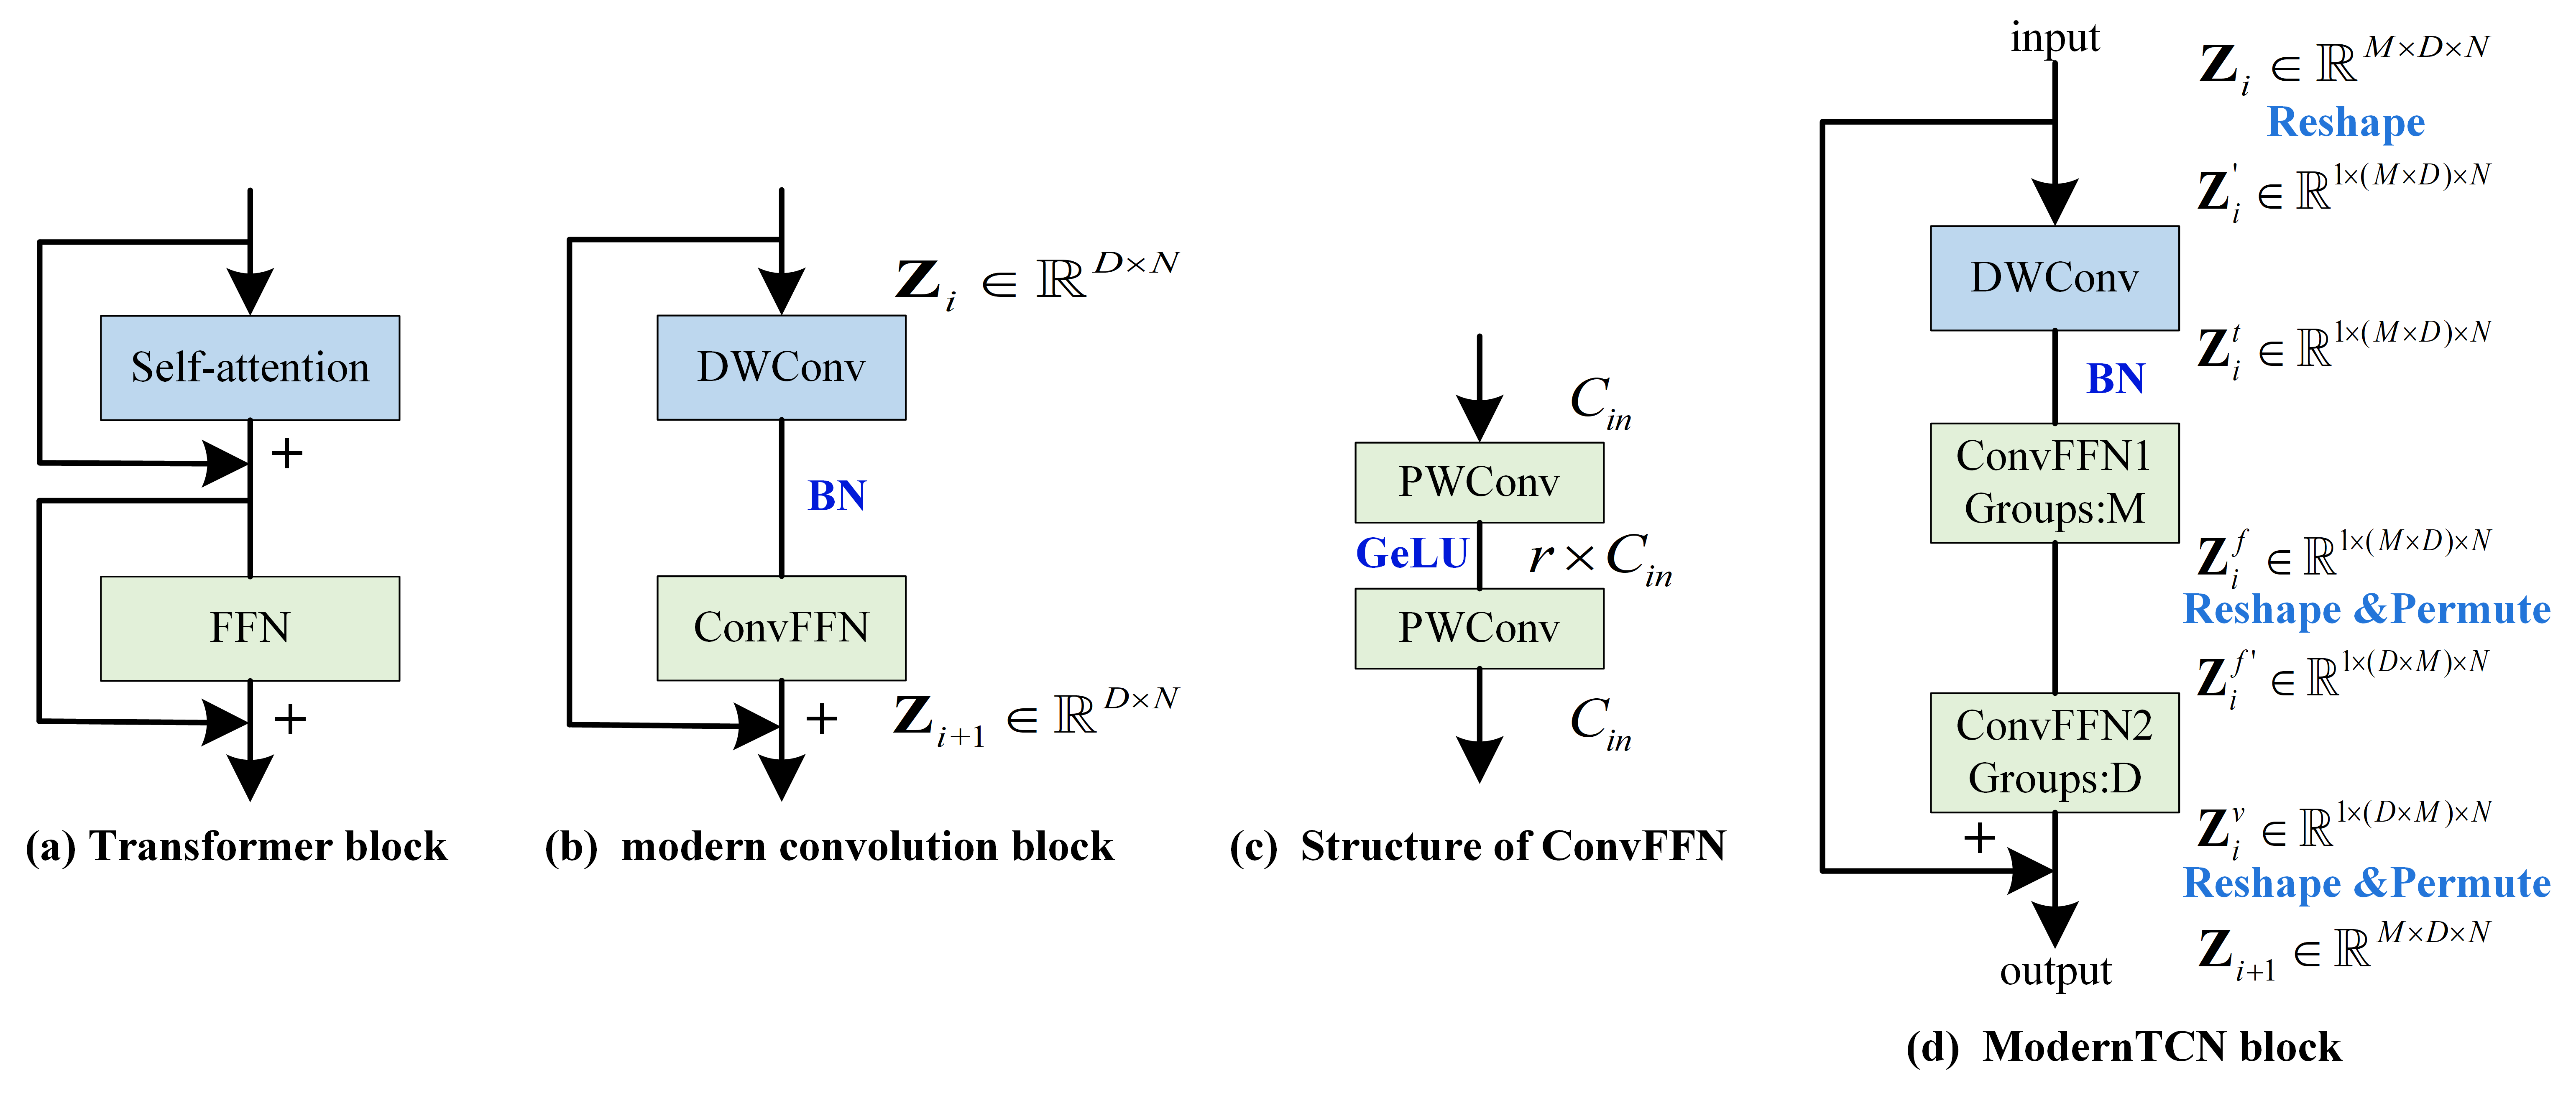
\includegraphics[width=\textwidth]{moderntcn_block.png}
    \caption{ModernTCN block design. The block separates temporal mixing (DWConv),
    per-variable feature learning (ConvFFN1), and cross-variable dependency capture
    (ConvFFN2) into three decoupled operations. $M$, $N$, and $D$ denote the variable,
    temporal, and feature dimensions respectively.
    Figure extracted from \citep{moderntcn2024}.}
    \label{fig:moderntcn_block}
\end{figure}

The first component, \textbf{DWConv}, is a depthwise convolution \citep{howard2017mobilenets} with a large kernel
--- by default size 51 --- applied independently per channel along the temporal
dimension. This is the component responsible for capturing temporal dependencies, and
the large kernel is what gives ModernTCN its wide effective receptive field. Each
channel operates independently here, so no information is mixed across variables or
features at this stage \citep{moderntcn2024}.

The second and third components together form a decoupled feed-forward network.
\textbf{ConvFFN1} mixes information across the feature dimension within each variable
independently, learning richer per-variable representations. \textbf{ConvFFN2} then
mixes information across the variable dimension per feature, capturing the
cross-variable (intermetric) dependencies that are critical for multivariate time
series \citep{moderntcn2024}. Decoupling these two operations --- rather than handling
them jointly --- reduces computational complexity and improves performance, as
confirmed by the authors' ablation studies \citep{moderntcn2024}.

\subsection{Anomaly Detection Approach}

ModernTCN applies the same \textbf{reconstruction-based} strategy as TimesNet for
anomaly detection. The model is trained to reconstruct normal input windows, and
anomalies are flagged at inference time based on reconstruction error exceeding a
threshold.


\section{TranAD}

TranAD \citep{tranad2022} is a transformer-based anomaly detection model for
multivariate time series.
Unlike TimesNet and ModernTCN, which are task-general backbones adapted for anomaly
detection among other tasks, TranAD is designed exclusively for anomaly detection
and diagnosis. It targets three practical challenges that are particularly relevant
to industrial and IoT settings: the absence of anomaly labels, high data volatility,
and the need for fast inference \citep{tranad2022}.

\subsection{Core Motivation}

The starting point for TranAD is a limitation shared by most recurrent models used
for anomaly detection: they process the input sequence one step at a time,
which makes training slow and limits their ability to capture long-range temporal
patterns. Transformers address both problems by processing the entire input window
in parallel through self-attention, making training substantially faster and giving
the model access to a much broader temporal context \citep{tranad2022}.

However, a plain transformer encoder-decoder is not sufficient on its own. Simple
reconstruction-based models tend to miss subtle anomalies --- those that deviate only
slightly from normal behaviour --- because the reconstruction error for near-normal
anomalies is too small to trigger detection. TranAD's central contribution is a
training procedure that deliberately amplifies these reconstruction errors, making
subtle anomalies easier to distinguish from normal data \citep{tranad2022}.

\subsection{Architecture}

TranAD's architecture, illustrated in Figure~\ref{fig:tranad_model}, consists of
two transformer encoders and two decoders. The model takes two inputs simultaneously:
the current input window $W$ and the complete sequence up to the current timestamp
$C$. The complete sequence gives the model a broad temporal context beyond the local
window, which is the key advantage over window-only models \citep{tranad2022}.

\begin{figure}[htbp]
    \centering
    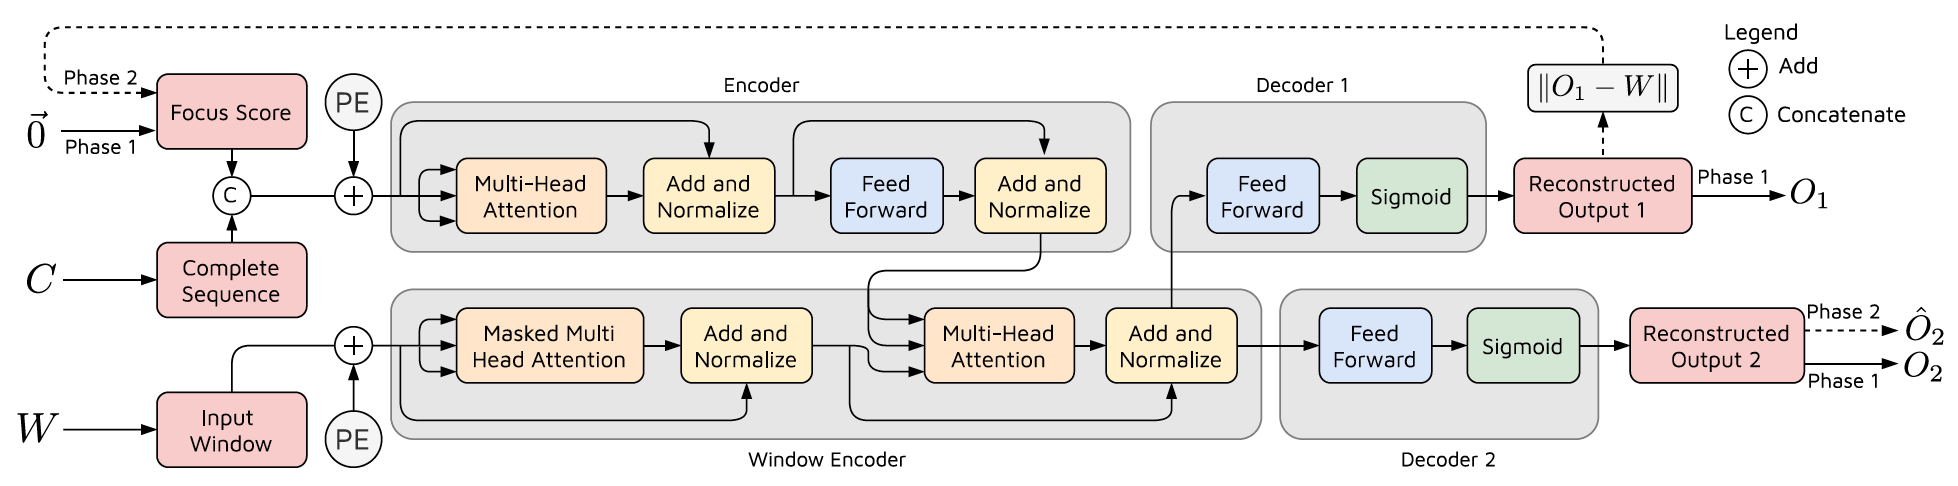
\includegraphics[width=\textwidth]{tranad_model.png}
    \caption{The TranAD model architecture. The model operates in two phases. In
    Phase~1, the input window $W$ and complete sequence $C$ are encoded and passed
    to two decoders to produce initial reconstructions $O_1$ and $O_2$. In Phase~2,
    the reconstruction error from $O_1$ is used as a focus score to re-condition
    the encoder, producing a refined reconstruction $\hat{O}_2$. The anomaly score
    is the average of the two reconstruction errors.
    Figure extracted from \citep{tranad2022}.}
    \label{fig:tranad_model}
\end{figure}

Inference proceeds in two phases. In the first phase, the model encodes both inputs
and produces two independent reconstructions of the input window. The deviation
between the first reconstruction and the actual input --- called the \textbf{focus
score} --- is then used to re-condition the encoder in the second phase. Specifically,
the focus score is fed back as an additional input signal that directs the model's
attention towards the parts of the sequence where the first reconstruction was least
accurate. The second phase then produces a refined reconstruction. This
\textbf{self-conditioning} mechanism serves two purposes: it amplifies reconstruction
errors in anomalous regions, making them easier to detect, and it helps the model
capture short-term temporal patterns that a single-pass reconstruction might miss
\citep{tranad2022}.

\subsection{Training}

The two decoders are trained \textbf{adversarially}. The first decoder tries to
reconstruct the input as accurately as possible --- in effect trying to produce a
zero focus score --- while the second decoder tries to maximise the difference between
its reconstruction and the input. This adversarial dynamic pushes the model to be
sensitive to even small deviations from normal behaviour. To keep training stable,
the loss function uses an \textbf{evolving weight} that starts by emphasising pure
reconstruction and gradually shifts weight towards the adversarial objective as the
reconstructions improve \citep{tranad2022}.

Additionally, TranAD incorporates \textbf{model-agnostic meta-learning}
\citep{finn2017maml}, which performs an additional gradient update at the end of each
epoch to help the model generalise quickly from limited training data. The authors
report that this component is particularly important when only a fraction of the
normal training data is available \citep{tranad2022}.

\subsection{Anomaly Detection Approach}

TranAD is a \textbf{reconstruction-based} model. At inference time, the anomaly
score for each window is defined as the average of the reconstruction errors from
the two phases. A timestamp is flagged as anomalous when this score exceeds a
threshold determined automatically using POT
\citep{siffer2017pot}. A timestamp is labelled anomalous if any of its $m$ dimensions
exceeds the threshold, which also enables \textbf{anomaly diagnosis} --- identifying
which specific sensor or variable is responsible for the anomaly.



\section{Anomaly Transformer}

Anomaly Transformer \citep{anomalytransformer2022} is a Transformer-based model for
unsupervised time series anomaly detection. Like TranAD, it is designed exclusively
for anomaly detection and leverages the self-attention mechanism of Transformers to
capture temporal associations across the full input window. However, the two models
differ fundamentally in their anomaly detection philosophy. Where TranAD amplifies
reconstruction errors through adversarial training, Anomaly Transformer introduces an
entirely different criterion: rather than measuring how poorly a time point is
reconstructed, it measures how differently a time point associates with the rest of
the series compared to what would be expected under normal conditions
\citep{anomalytransformer2022}.

\subsection{Association Discrepancy}

The central insight of Anomaly Transformer is rooted in a structural property of
anomalies: because anomalies are rare and dominated by surrounding normal data, it is
extremely difficult for an anomalous time point to build meaningful associations with
the entire series. Instead, its attention will tend to concentrate on its immediate
temporal neighbours, which are more likely to share a similar abnormal pattern due to
the continuity of the signal. Normal time points, by contrast, can discover informative
associations with distant parts of the series, not just the adjacent area
\citep{anomalytransformer2022}.

This observation leads to the concept of \textbf{Association Discrepancy}: the
difference between a time point's \textit{prior-association} --- a learnable Gaussian
kernel that encodes an adjacent-concentration inductive bias --- and its
\textit{series-association} --- the self-attention weights learned from the raw series.
Because anomalies are forced to concentrate their attention locally while normal points
spread it more broadly, anomalous time points will exhibit a smaller association
discrepancy than normal ones. This makes the association discrepancy an inherently
distinguishable criterion between normal and abnormal behaviour, without requiring
any anomaly labels \citep{anomalytransformer2022}.


\subsection{Architecture}

The overall architecture of Anomaly Transformer, shown in
Figure~\ref{fig:anomaly_transformer_arch}, stacks $L$ identical blocks, each
consisting of an \textbf{Anomaly-Attention} mechanism followed by a feed-forward
layer with residual connections and layer normalisation. The key departure from a
vanilla Transformer is the Anomaly-Attention mechanism itself, which replaces the
standard single-branch self-attention with a \textbf{two-branch structure}
\citep{anomalytransformer2022}.

\begin{figure}[htbp]
    \centering
    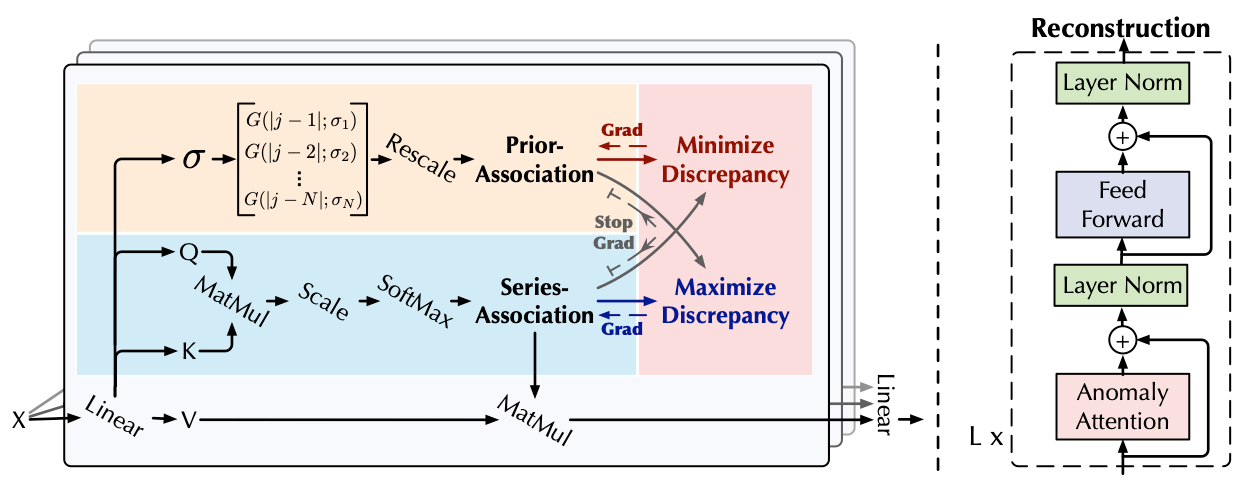
\includegraphics[width=\textwidth]{anomalytransformer.png}
    \caption{Anomaly Transformer architecture. The Anomaly-Attention mechanism (left)
    contains two branches: the prior-association (orange), computed via a learnable
    Gaussian kernel applied to the learned scale $\sigma$, and the series-association
    (blue), computed via standard scaled dot-product self-attention. The minimax
    strategy drives the two branches apart via opposing gradient directions (red and
    blue arrows), with a stop-gradient mechanism (grey) ensuring each phase only
    updates its own branch. The reconstruction output is produced from the
    series-association branch by multiplying with $V$. The overall model (right)
    stacks $L$ such Anomaly-Attention blocks residually.
    Figure extracted from \citep{anomalytransformer2022}.}
    \label{fig:anomaly_transformer_arch}
\end{figure}

As visible in Figure~\ref{fig:anomaly_transformer_arch}, the input $X$ is projected
linearly into queries $Q$, keys $K$, values $V$, and a scale parameter $\sigma$. The
two branches then operate in parallel on these projections.

The \textbf{prior-association branch} (orange region) uses $\sigma$ to compute, for
each time point $i$, a Gaussian kernel $G(|j - i|; \sigma_i)$ over all other time
points $j$. This produces a distribution that is unimodal and centred on $i$,
naturally concentrating weight on nearby time points. The learnable scale $\sigma_i$
controls how broadly or narrowly the kernel spreads, allowing the model to adapt the
prior to different temporal patterns. The resulting association weights are rescaled
to form a proper discrete distribution \citep{anomalytransformer2022}.

The \textbf{series-association branch} (blue region) is a standard scaled
dot-product attention map: $Q$ and $K$ are multiplied, scaled, and passed through
softmax to produce association weights over the full sequence. The reconstruction of
the input is then obtained by multiplying these weights with $V$, following the
standard Transformer formulation. Crucially, this branch learns its associations
directly from the data, without any imposed locality constraint
\citep{anomalytransformer2022}.

The \textbf{association discrepancy} is computed as the symmetrised KL divergence
between the prior-association and the series-association at each time point, averaged
across all $L$ layers. The final anomaly score multiplies this discrepancy with the
point-wise reconstruction error, so that both signals collaborate: a time point with
a small association discrepancy is down-weighted in the reconstruction error term,
making the combined score more robust than either criterion alone
\citep{anomalytransformer2022}.



\subsection{Anomaly Detection Approach}

Anomaly Transformer is a \textbf{reconstruction-based} model augmented with an
association-based criterion. During unsupervised training on normal data, the model
learns to reconstruct input windows while simultaneously maximising the association
discrepancy between normal and anomalous patterns. At
inference time, each time point receives a scalar anomaly score combining its
reconstruction error and its normalised association discrepancy. A time point is
flagged as anomalous when this score exceeds a threshold, determined from the
validation set by selecting the proportion of data to label as anomalous
\citep{anomalytransformer2022}.



\section{GTA}

GTA \citep{gta2022} is a multivariate time series anomaly detection framework
designed explicitly for IoT settings. Unlike the models discussed so far ---
TimesNet, ModernTCN, TranAD, and Anomaly Transformer --- which treat the
input sensors as independent channels or as a flat multivariate vector, GTA
starts from the observation that IoT sensors are not independent: they are
embedded in a physical system with a real but unknown topological structure.
Opening a valve in a water treatment plant changes pressure readings downstream;
an attack on one sensor propagates through the network in a chain. The central
argument of GTA is that explicitly modelling these inter-sensor dependencies
--- rather than leaving them implicit in a flat attention map --- is essential
for accurate anomaly detection in such settings \citep{gta2022}.

\subsection{Graph Structure Learning}

The challenge is that while the dependency structure between sensors is real,
it is not known in advance. In most IoT deployments, the internal mechanisms
linking sensors are hidden --- operators may know that sensors are related, but
not precisely how, or in which direction influence flows. GTA therefore needs
to \textit{discover} the graph structure from the data itself rather than
assuming it \citep{gta2022}.

GTA learns this structure \textbf{end-to-end} during training. Each sensor is
modelled as a node in a directed graph, and for each ordered pair of sensors
$(i, j)$, the model learns a probability that information should flow from
sensor $i$ to sensor $j$. Because directly sampling a binary connection
decision is non-differentiable and would block gradient flow, GTA uses a
\textbf{Gumbel-Softmax Sampling} strategy: a continuous, differentiable
relaxation of the discrete decision that allows the connection structure to be
optimised jointly with the rest of the model through standard backpropagation
\citep{gta2022}.

Crucially, GTA does not simply connect every sensor to every other sensor. A
fully connected graph would aggregate information from all neighbours
indiscriminately, adding noise and obscuring the meaningful signal. Instead, a
\textbf{sparsity regularisation} term penalises the total number of established
connections, pushing the model to retain only the most informative links for
each node \citep{gta2022}. The resulting graph is sparse, computationally
efficient to use in the downstream convolution layers, and physically
interpretable: in the authors' case study on a cyber-attack dataset, the
discovered graph closely matched the known physical relationships between
sensors, with malicious influence correctly traced from attacked upstream nodes
to affected downstream ones \citep{gta2022}.

\subsection{Architecture}

The overall architecture of GTA, illustrated in Figure~\ref{fig:gta_arch},
combines two main components that process the input in sequence: a
\textbf{hierarchical context encoding block} and a \textbf{Transformer
encoder-decoder} \citep{gta2022}.

\begin{figure}[htbp]
    \centering
    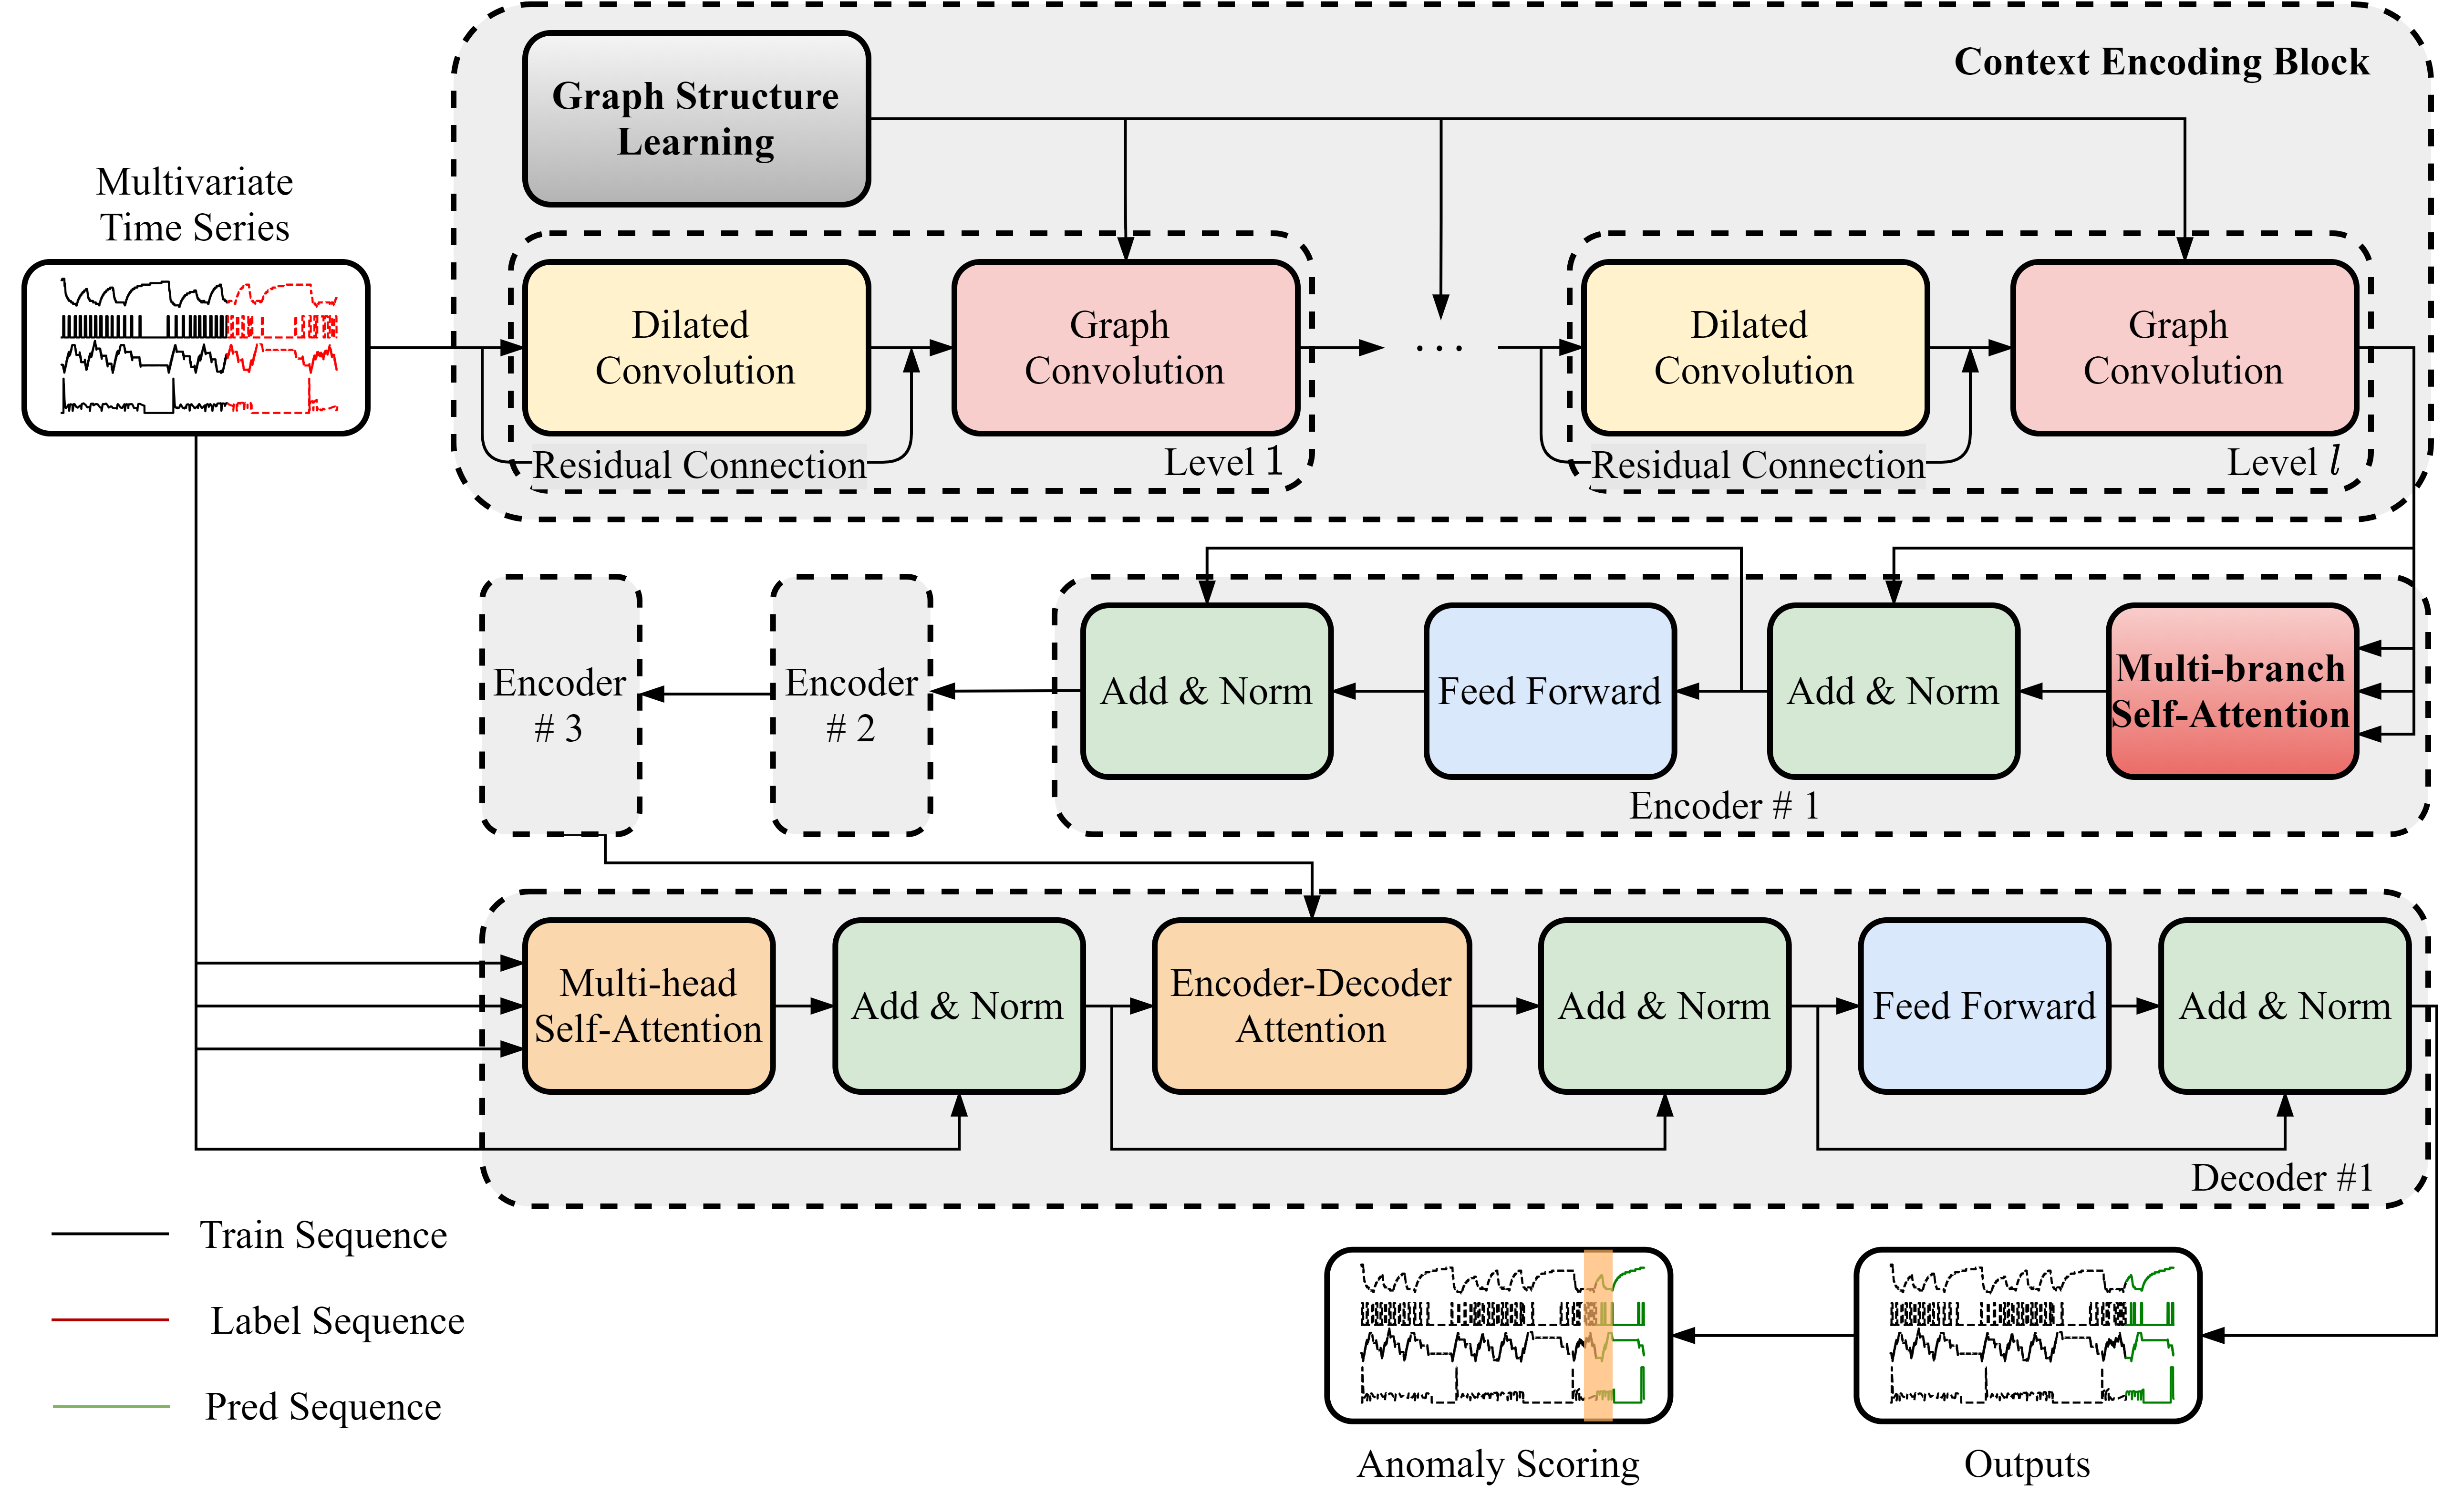
\includegraphics[width=\textwidth]{gta.png}
    \caption{The GTA architecture. The input multivariate time series is first
    processed through a hierarchical context encoding block that interleaves
    multi-scale dilated convolutions with Influence Propagation graph convolutions
    to produce spatiotemporal embeddings. These are then fed into a
    Transformer-based encoder-decoder for single-step forecasting.
    Figure extracted from \citep{gta2022}.}
    \label{fig:gta_arch}
\end{figure}

\paragraph{Hierarchical context encoding.}
The context encoding block is the spatial-temporal heart of GTA. It interleaves
two operations in a hierarchical, multi-scale fashion: \textbf{dilated
convolutions} \citep{yu2016dilated} for temporal modelling and \textbf{Influence
Propagation (IP) graph convolution} for spatial modelling \citep{gta2022}.

The dilated convolutions operate along the temporal dimension with increasing
dilation rates across levels, allowing the model to capture temporal patterns
at multiple scales --- short-range patterns at the first level, longer-range
patterns at subsequent levels --- without a proportionally large number of
parameters \citep{gta2022}. The outputs of each dilated convolution level are
then passed through an IP graph convolution that propagates information across
the learned sensor graph. The IP convolution is designed to model
\textit{influence propagation}: rather than simply averaging neighbour
representations, it computes the difference between each pair of connected
sensors' time series embeddings, explicitly modelling how a change at one
sensor flows to downstream neighbours \citep{gta2022}. This is physically
motivated --- anomalies in IoT systems typically cascade through the network
rather than appearing in isolation.

\paragraph{Transformer-based forecasting.}
The spatiotemporal representations produced by the context encoding block are
fed into a Transformer encoder-decoder that performs single-step forecasting:
predicting the next timestamp's sensor values from the encoded historical
context \citep{gta2022}. The Transformer here plays the same role as in TranAD
and Anomaly Transformer --- processing the full sequence in parallel and
capturing long-range temporal dependencies through self-attention --- but is
used for prediction rather than reconstruction.

One practical modification is made to the standard multi-head self-attention
mechanism to reduce its quadratic cost. GTA introduces a \textbf{multi-branch
attention} mechanism: the input embedding is split along the channel dimension
into two branches, each handled by a different type of attention. One branch
uses standard pairwise attention for capturing local temporal patterns, while
the other uses a fixed globally-learned matrix that does not depend on the
input and therefore requires no query-key dot products \citep{gta2022}. The
two branches are then concatenated to form the final attention output. This
reduces the overall computational cost while retaining the model's ability to
capture both local and global temporal patterns --- a deliberate design choice
motivated by the efficiency requirements of IoT deployments \citep{gta2022}.

\subsection{Anomaly Detection Approach}

GTA is a \textbf{forecasting-based} model, which sets it apart from all other
models in this thesis --- TimesNet, ModernTCN, TranAD, and Anomaly Transformer
are all reconstruction-based. Rather than reconstructing the current input window
and measuring reconstruction error, GTA learns to predict the next timestamp's
sensor values from historical context. At inference time, the anomaly score for
each timestamp is the mean squared error between the model's prediction and the
actual observed values across all sensors \citep{gta2022}. A timestamp is flagged
as anomalous when this score exceeds a threshold. Because the model is trained
exclusively on normal data, it learns to predict normal sensor behaviour
accurately; anomalies produce large prediction errors because they deviate from
the patterns the model has learned.



%%%%%%%%%%%%%%%%%%%%%%%%%%%%%%%%%%%%%%%%%%%%%%%%%%%%%%%%%%%%%%%%%%%%%%%

\chapter{Experiments}

The evaluation framework used in this thesis is designed around two complementary 
objectives: assessing detection accuracy and assessing suitability for IoT edge 
deployment.
Deploying AI models on edge devices faces significant challenges, including 
limited computing power, restricted memory budgets, and real-time processing requirements 
\citep{wang2025optimizing}, and a model that achieves high detection accuracy but is 
computationally intractable or memory-prohibitive on constrained hardware is of limited 
practical value in the target setting. For this reason, accuracy metrics are reported 
alongside a comprehensive set of efficiency metrics covering computational cost, memory 
footprint, and inference speed. 

On the accuracy side, Precision, Recall, and F1 Score 
capture point-wise detection quality, with F1 serving as the primary comparison metric 
since it is universally reported in the papers of all five evaluated models and provides 
a balanced view of both false alarms and missed detections \citep{darban2024survey}. 
F1 scores are computed under the point-adjust (PA) protocol \citep{xu2018donut}, which 
is the standard convention in the TSAD literature and is adopted by all baseline results 
compared in this thesis, ensuring fair cross-model comparison 
\citep{xu2022detectionadjustment}. The Area Under the Precision-Recall Curve (AU-PR) 
is additionally reported without point adjustment, providing a threshold-independent and 
inflation-free complementary perspective that is particularly informative on the heavily 
imbalanced datasets used here \citep{darban2024survey}. 

On the efficiency side, 
Multiply-Accumulate Operations (MACs) quantify the hardware-independent computational 
cost of a forward pass, measured using \texttt{fvcore} \citep{fvcore} with custom 
operator handlers where needed; five memory metrics capture different aspects of the 
model's memory demand from minimum storage cost to peak runtime footprint; and latency 
and throughput characterise how quickly each model can process incoming sensor data, 
which directly determines whether it can sustain real-time inference on a resource-limited 
edge device \citep{wang2025optimizing}.

All experiments were conducted on a server running Ubuntu 24.04.2 LTS, 
equipped with two Intel Xeon E5-2620 v4 
processors (8 cores per socket, 2 threads per core, 2.10\,GHz base clock, 
3.00\,GHz boost), yielding 32 logical CPU cores in total, and 128\,GB of system 
RAM. The server is fitted with four NVIDIA GeForce RTX 2080 GPUs, each with 
8\,GB of VRAM. TranAD, whose codebase hardcodes CPU execution, 
ran exclusively on the server CPUs.

TODO: EDGE DEVICE SPECS

\section{Datasets}

The statistics of the 5 selected datasets are provided in Table~\ref{tab:dataset_stats}.

\paragraph{Server Machine Dataset (SMD).}

The Server Machine Dataset (SMD) \cite{su2019smd} is a real-world multivariate time series dataset
collected from a large Internet company. It contains five weeks of resource utilisation traces
from 28 server machines, covering 38 dimensions per machine.
The anomaly rate refers to the proportion of time steps in the dataset that are labelled as
anomalous. For SMD, this is approximately 4.2\%, meaning
that the vast majority of observations reflect normal server behaviour, with anomalous events
being relatively rare. 

\paragraph{Mars Science Laboratory (MSL).}

The Mars Science Laboratory (MSL) \cite{hundman2018smap} dataset is a publicly available NASA dataset
containing telemetry anomaly data derived from the Incident
Surprise Anomaly (ISA) reports of spacecraft monitoring systems.
It records sensor and actuator data from the Mars rover itself, covering 55 dimensions. 
The anomaly rate is approximately 10.48\%, meaning that a substantially larger
proportion of time steps are labelled anomalous compared to SMD. MSL is one of the
most widely used benchmarks in the TSAD literature and
is commonly evaluated alongside SMAP dataset, both originating from the
same NASA spacecraft monitoring programme.

\paragraph{Soil Moisture Active Passive (SMAP).}

The Soil Moisture Active Passive (SMAP) dataset \cite{hundman2018smap}
is a publicly available NASA dataset, released alongside MSL and originating from the same
spacecraft monitoring programme. It contains telemetry anomaly data derived from the
Incident Surprise Anomaly (ISA) reports of the SMAP satellite, covering measurements
such as radiation, temperature, and power, across 25 dimensions. 
The anomaly rate is approximately 12.83\%. 

\paragraph{Secure Water Treatment (SWaT).}

The Secure Water Treatment (SWaT) dataset \cite{mathur2016swat} is collected from a
real-world water treatment testbed operated for cyber-attack investigation. The data
collection process lasted 11 days, with the system operated continuously such that
all values from all 51 sensors and actuators were recorded. The first
7 days of operation were conducted under normal conditions, while the remaining 4
days involved 41 distinct attacks derived from a model of the intent space of a
cyber-physical system. The dataset covers sensor
measurements such as water level and flow rate, as well as actuator operations such
as valves and pumps. The anomaly rate is approximately 12.14\%. 
Unlike the NASA spacecraft datasets, SWaT exhibits strong
topological dependencies between sensors, as any change in one sensor can propagate
through the network to other sensors \cite{gta2022}.

\paragraph{Pooled Server Metrics (PSM).}

The Pooled Server Metrics (PSM) dataset \cite{abdulaal2021psm} is a real-world
multivariate time series dataset collected internally from multiple application
server nodes at eBay. It covers 25 dimensions of
server performance metrics. The anomaly rate is
approximately 27.76\%, meaning that more than a quarter
of the test set time steps are labelled anomalous.

\begin{table}[ht]
\centering
\caption{Dataset Statistics}
\label{tab:dataset_stats}
\begin{tabular}{llrrrrrr}
\toprule
\textbf{Dataset} & \textbf{Domain} & \textbf{Dim.} 
    & \textbf{Train} & \textbf{Test} & \textbf{Anom. Rate (\%)} \\
\midrule
SMD  & Server machines  & 38 & 566,724 & 708,420 & 4.20 \\
MSL  & Spacecraft       & 55 &  44,653 &  73,729 & 10.48 \\
SMAP & Spacecraft       & 25 & 108,146 & 427,617 & 12.83 \\
SWaT & Water treatment  & 51 & 396,000 & 449,919 & 12.14 \\
PSM  & Server machines  & 25 & 105,984 &  87,841 & 27.76 \\
\bottomrule
\end{tabular}
\end{table}

\section{Results}

All models were trained and evaluated following the experimental setup described in their respective publications, 
with the goal of reproducing the best performance reported by their authors. Where a paper explicitly specified 
hyperparameter values, those values were used directly. For hyperparameters not described in a paper, 
the default values provided in the model's official repository were adopted. This approach was chosen to ensure 
that comparisons reflect each model's intended operating point rather than an arbitrarily tuned configuration, 
and to expose any discrepancies between reported and reproducible performance. Training procedures, including 
the number of epochs, learning rate schedules, and data preprocessing steps, were likewise kept consistent 
with each paper's specification wherever possible.

\subsection{F1 score and AU-PR}

Table~\ref{tab:accuracy} reports the precision, recall, F1 score, and area under the precision-recall curve (AU-PR) 
for all five models across the five benchmark datasets, together with the macro-average F1 and AU-PR computed over all datasets. 

\begin{table}[ht]
\centering
\caption{Detection accuracy (Precision, Recall, F1, and AU-PR in \%) across five benchmark datasets. 
Best F1 and AU-PR per dataset in \textbf{bold}, second-best \underline{underlined}.}
\label{tab:accuracy}
\begin{tabular}{ll rrrrr}
\toprule
\textbf{Dataset} & \textbf{Metric} $\uparrow$ & \thead{\textbf{TimesNet}\\\citep{timesnet2023}} & \thead{\textbf{ModTCN}\\\citep{moderntcn2024}} & \thead{\textbf{TranAD}\\\citep{tranad2022}} & \thead{\textbf{AnomTr.}\\\citep{anomalytransformer2022}} & \thead{\textbf{GTA}\\\citep{gta2022}} \\
\midrule
\multirow{4}{*}{SMD}
    & Precision & 87.57 & 86.84 & 90.72 & 89.41 & 86.17 \\
    & Recall    & 80.35 & 80.01 & 99.73 & 96.20 & 95.67 \\
    & F1        & 83.80 & 83.28 & \textbf{95.01} & \underline{92.68} & 90.67 \\
    & AU-PR     & 14.90 & 14.20 & \textbf{50.19} &  4.45 & \underline{15.82} \\
\midrule
\multirow{4}{*}{MSL}
    & Precision & 87.04 & 89.39 & 90.38 & 98.89 & 91.69 \\
    & Recall    & 71.40 & 74.80 & 99.99 & 98.00 & 84.24 \\
    & F1        & 78.45 & 81.45 & \textbf{94.95} & \underline{94.91} & 87.81 \\
    & AU-PR     & \underline{14.85} & 14.80 & \textbf{16.59} & 10.42 & 11.62 \\
\midrule
\multirow{4}{*}{SMAP}
    & Precision & 89.49 & 90.29 & 80.43 & 93.67 & 73.66 \\
    & Recall    & 55.44 & 53.85 & 99.99 & 99.32 & 78.48 \\
    & F1        & 68.47 & 67.46 & \underline{89.15} & \textbf{96.41} & 76.00 \\
    & AU-PR     & 11.86 & 11.36 & 10.16 & \textbf{12.90} & \underline{12.33} \\
\midrule
\multirow{4}{*}{SWaT}
    & Precision & 90.29 & 95.85 & 99.77 & 98.88 & 90.27 \\
    & Recall    & 95.41 & 86.97 & 68.79 & 87.00 & 88.36 \\
    & F1        & \textbf{92.78} & 91.19 & 81.43 & \underline{92.56} & 89.31 \\
    & AU-PR     & 10.81 &  9.60 & \textbf{73.66} & \underline{11.10} &  8.62 \\
\midrule
\multirow{4}{*}{PSM}
    & Precision & 98.37 & 98.74 & 89.44 & 97.16 & 99.27 \\
    & Recall    & 93.46 & 94.32 & 85.63 & 97.47 & 93.71 \\
    & F1        & 95.85 & \underline{96.48} & 87.50 & \textbf{97.31} & 96.41 \\
    & AU-PR     & 37.80 & \underline{38.29} & \textbf{46.01} & 28.84 & 34.97 \\
\midrule
\multirow{2}{*}{Average}
    & F1        & 83.87 & 83.97 & \underline{89.61} & \textbf{94.77} & 88.04 \\
    & AU-PR     & \underline{18.04} & 17.65 & \textbf{39.32} & 13.54 & 16.67 \\
\bottomrule
\end{tabular}
\end{table}

Across the five datasets, TranAD \citep{tranad2022} and Anomaly Transformer \citep{anomalytransformer2022} consistently achieve the highest F1 scores. 
TranAD attains the best F1 on SMD (95.01\%) and MSL (94.95\%), driven by near-perfect recall on both datasets (99.73\% and 99.99\%, respectively), 
which is characteristic of its adversarial training objective and self-conditioning mechanism designed to amplify reconstruction deviations \citep{tranad2022}. 
Anomaly Transformer leads on SMAP (96.41\%) and PSM (97.31\%), where its association-discrepancy criterion produces strong separation between normal and 
anomalous time points \citep{anomalytransformer2022}. On SWaT, TimesNet achieves the highest F1 (92.78\%), marginally ahead of Anomaly Transformer (92.56\%) and ModernTCN (91.19\%).

In terms of average F1, Anomaly Transformer ranks first (94.77\%), closely followed by TranAD (89.61\%) and GTA (88.04\%), while TimesNet (83.87\%) 
and ModernTCN (83.97\%) trail slightly behind. The two convolutional models --- TimesNet \citep{timesnet2023} and ModernTCN \citep{moderntcn2024} 
--- show very similar profiles across all datasets, with consistently high precision but lower recall on the more challenging SMAP dataset.

The AU-PR results tell a notably different story. While all models achieve high F1 under point adjustment, AU-PR values are substantially lower across 
the board, reflecting the difficulty of maintaining precision across the full range of anomaly score thresholds on heavily imbalanced test sets 
\citep{darban2024survey}. TranAD stands out with the highest average AU-PR (39.32\%), largely owing to its strong SWaT (73.66\%) and SMD (50.19\%) results. 
All other models cluster between 13 and 18\% in average AU-PR, with Anomaly Transformer notably low at 13.54\% despite its leading average F1. This divergence 
between F1 and AU-PR highlights the sensitivity of point-adjusted F1 to threshold selection, and underscores the value of reporting AU-PR as a complementary, 
threshold-independent measure of detection quality \citep{darban2024survey}.


Figure~\ref{fig:f1_barchart} and Figure~\ref{fig:aupr_barchart} complement the per-dataset results in 
Table~\ref{tab:accuracy} by visualising the distribution of F1 and AU-PR scores across datasets for 
each model, making consistency and variance across benchmarks directly comparable.

\begin{figure}[ht]
    \centering
    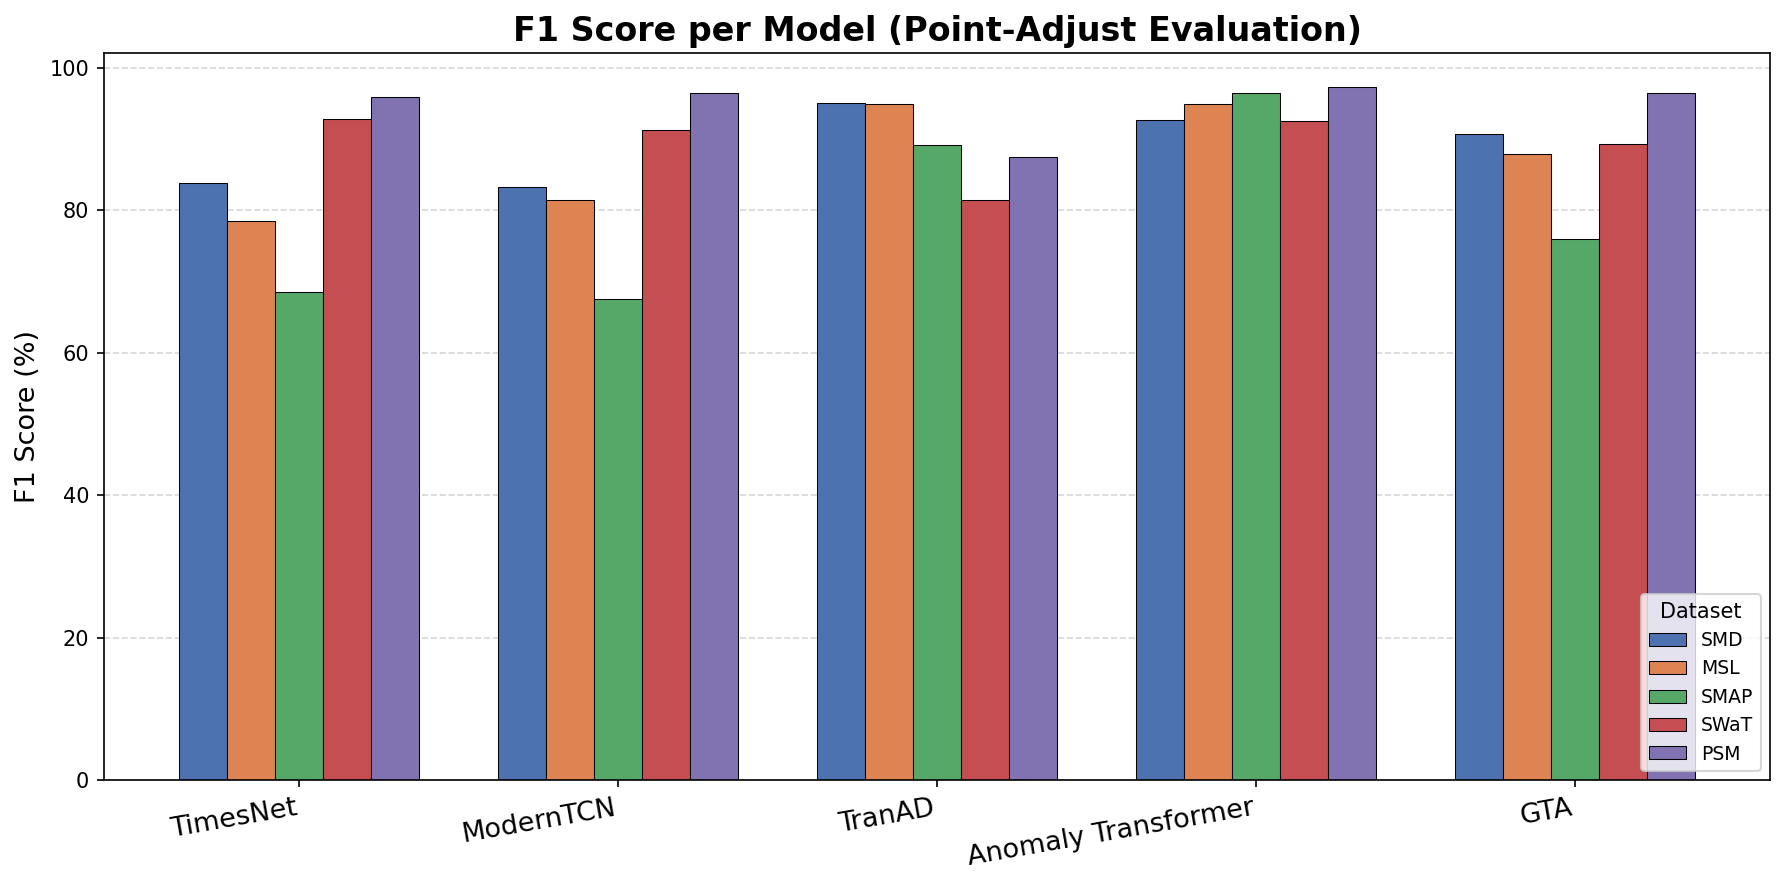
\includegraphics[width=\textwidth]{f1_barchart_by_model.png}
    \caption{F1 score distribution per model across the five benchmark datasets under the 
    point-adjust evaluation protocol. Each bar represents a single dataset result.}
    \label{fig:f1_barchart}
\end{figure}

\begin{figure}[ht]
    \centering
    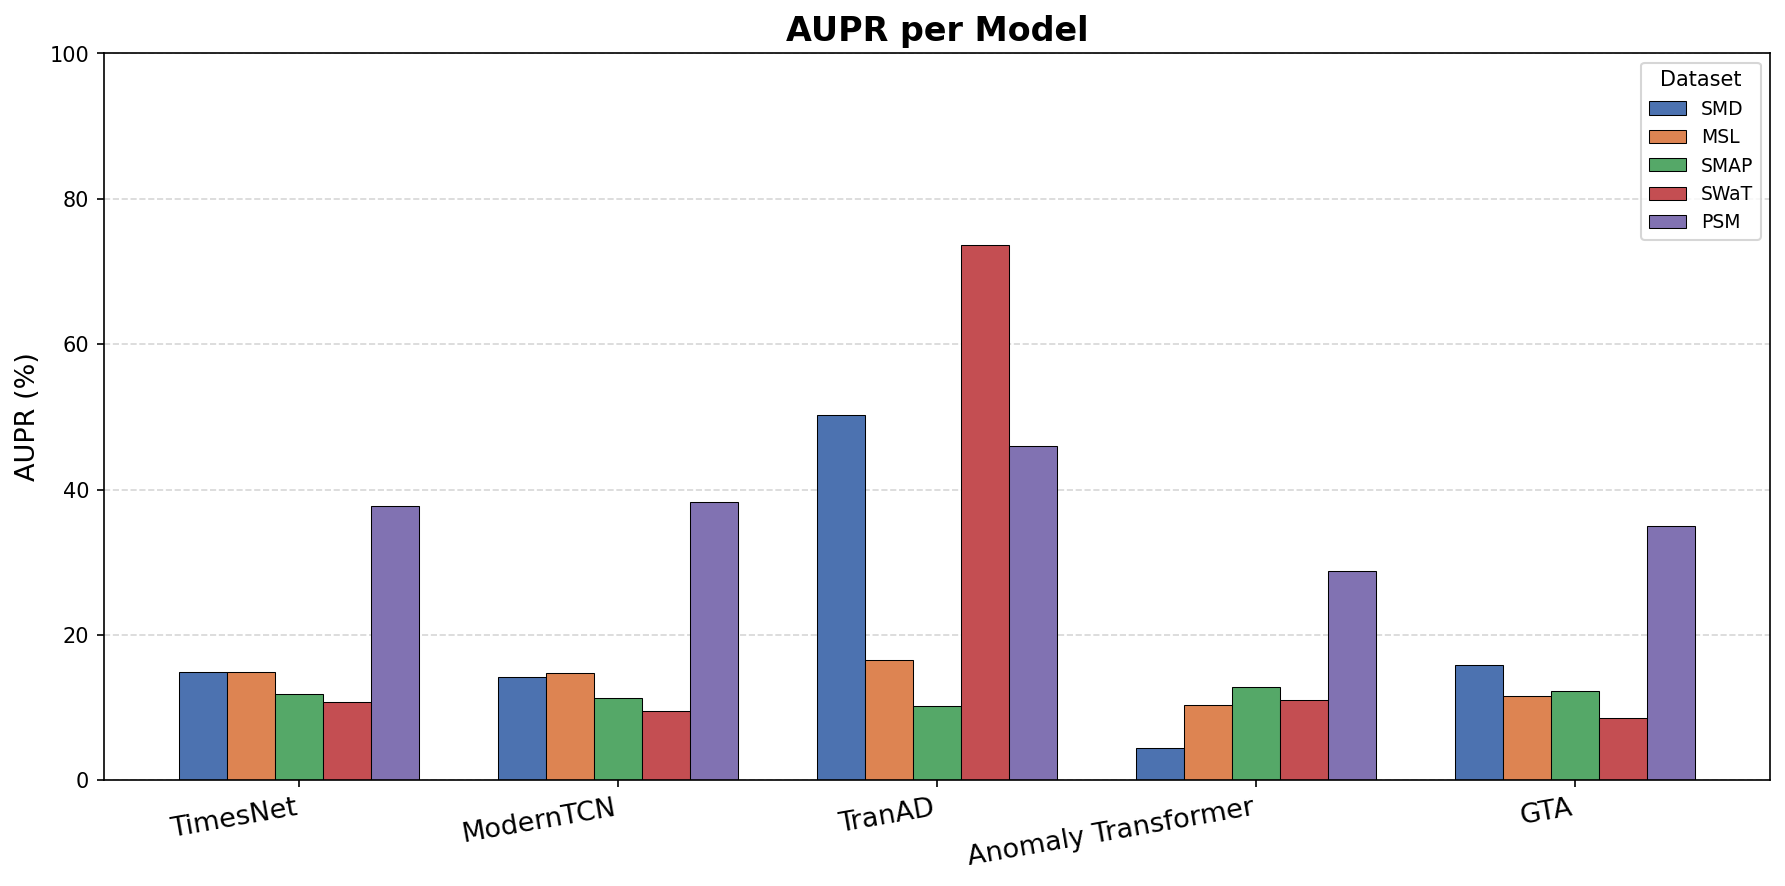
\includegraphics[width=\textwidth]{aupr_barchart_by_model.png}
    \caption{AU-PR distribution per model across the five benchmark datasets. 
    Each bar represents a single dataset result.}
    \label{fig:aupr_barchart}
\end{figure}

Figure~\ref{fig:f1_barchart} and Figure~\ref{fig:aupr_barchart} complement the 
per-dataset results in Table~\ref{tab:accuracy} by enabling direct visual 
comparison of F1 and AU-PR scores across models and datasets.

Anomaly Transformer achieves the highest scores and the most 
consistent performance, with values between 92\% and 97\% across all datasets. 
TranAD shows a wider spread, reflecting its strong performance on SMD and MSL contrasted with 
a notably lower F1 on SWaT (81.43\%). TimesNet and ModernTCN exhibit very similar profiles, 
both characterised by wide spread driven by their weak performance on SMAP (68.47\% and 
67.46\% respectively), which appears as a clear low outlier for both models. GTA presents a 
relatively compact spread with high scores on most datasets, though it similarly struggles on 
SMAP (76.00\%), while its PSM result (96.41\%) sits at the upper end.

The AU-PR bar chart tells a strikingly different story. Four of the five models --- TimesNet, 
ModernTCN, Anomaly Transformer, and GTA --- show AU-PR values 
between roughly 8\% and 16\% across most datasets, with PSM as a consistent positive outlier for all of them. This 
reveals that, despite their differing F1 profiles, these models perform similarly poorly in 
terms of threshold-independent detection quality across most datasets. TranAD is a clear 
exception: its bars are widely spread from approximately 10\% to 74\%, with its SWaT AU-PR 
of 73.66\% standing far above all other results, driving both its superior average AU-PR and 
the large variance visible in the plot. Notably, Anomaly Transformer's SMD AU-PR (4.45\%) 
sits far below its other results, highlighting that its high F1 on that dataset is highly 
sensitive to threshold choice. Taken together, the two plots suggest that high point-adjusted 
F1 and high AU-PR are not interchangeable: a model can rank first on F1 while performing near 
the bottom on AU-PR, reinforcing the importance of reporting both metrics \citep{darban2024survey}.

\subsubsection{What's behind TranAD's high AU-PR on SWaT}
Figure~\ref{fig:pr_all_swat} shows the precision-recall curves for all five models on the 
SWaT dataset alongside the no-skill baseline.

\begin{figure}[ht]
    \centering
    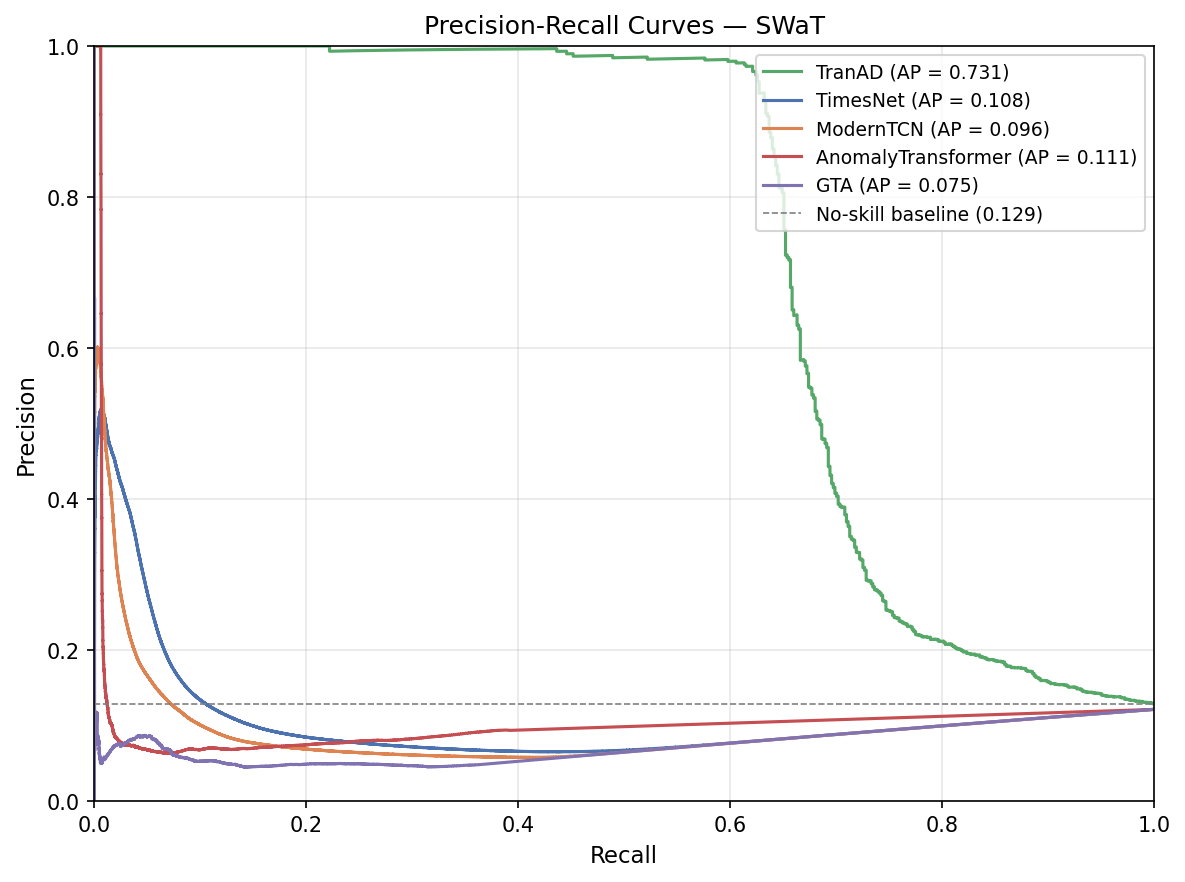
\includegraphics[width=\textwidth]{pr_curves_all_SWaT.png}
    \caption{Precision-recall curves for all five models on SWaT. The dashed line 
    indicates the no-skill baseline equal to the dataset's anomaly rate (12.9\%).}
    \label{fig:pr_all_swat}
\end{figure}

A precision-recall curve is constructed by sweeping the anomaly score threshold from its highest 
value (flagging almost nothing) to its lowest (flagging everything). Moving left to right along the curve 
corresponds to lowering the anomaly score threshold and accepting more detections. A high area 
under the curve represents both high recall and high precision: high precision is achieved by 
having few false positives in the returned results, and high recall by having few false negatives 
among all anomalous points \citep{sklearn_pr_curve}. A system with high precision but low recall 
returns very few detections but most of its predicted labels are correct; a system with high 
recall but low precision returns most of the relevant anomalies but the proportion of false alarms 
among the returned results is high \citep{sklearn_pr_curve}. The 
no-skill baseline --- shown as the dashed horizontal line at 0.129 --- represents a random 
classifier that flags anomalies at the dataset's base rate; any useful model must remain 
substantially above this line. The area under the full curve (AU-PR, here equal to 0.731) 
summarises performance across all thresholds into a single scalar, making it a 
threshold-independent measure of detection quality \citep{darban2024survey}.

\paragraph{What the curve reveals for TranAD on SWaT.}
The curve has a distinctive L-shape. From recall 0.0 to approximately 0.6, precision remains 
near 1.0, meaning that at high thresholds TranAD flags very few points but almost all of them 
are true anomalies. This reflects TranAD's adversarial self-conditioning mechanism, which 
produces large, concentrated reconstruction errors on genuinely anomalous windows in 
SWaT \citep{tranad2022}. The steep vertical drop around recall 0.6--0.65 marks the point at 
which the threshold crosses into regions where normal and anomalous score distributions begin 
to overlap, causing precision to collapse rapidly. Beyond recall 0.65, the curve descends 
gradually towards the baseline, indicating that recovering the remaining anomalous points 
requires accepting a large number of false positives.

In contrast, TimesNet (AP = 0.108), ModernTCN (AP = 0.096), Anomaly Transformer 
(AP = 0.111), and GTA (AP = 0.075) all collapse towards or below the no-skill baseline almost 
immediately, their curves indistinguishable from a random classifier across most of the recall 
range. This confirms that for these four models, any threshold that recovers a meaningful 
fraction of anomalies does so at the cost of flagging nearly as many normal points. TranAD's 
AP of 0.731 therefore does not just represent a quantitative improvement --- it reflects a 
qualitatively different level of score separability on this dataset, further reinforcing why 
AU-PR exposes differences between models that point-adjusted F1 alone would conceal 
\citep{darban2024survey}.


\paragraph{Confusion Matrix.}

Figure~\ref{fig:cm_tranad_swat} shows the confusion matrix for TranAD on SWaT. 
Out of the total anomalous points in the test set, only 4.5\% 
are flagged as anomalous (true positives), while 8.4\%  are missed entirely (false negatives). At 
the same time, only 1 normal point (0.0002\%) is incorrectly flagged as anomalous (false positive), and 
87.1\%  normal points are correctly identified as normal (true negatives).

TranAD almost never raises a false alarm (only 1 false positive), but as a consequence misses 
nearly two thirds of all anomalous points at the point level. It is important to note that 
these are raw point-level counts without point adjustment applied. Under the point-adjust 
protocol, any anomaly segment in which at least one point is correctly flagged is credited as 
fully detected \citep{su2019smd}, which substantially changes the effective recall and explains 
why the PA F1 reported in Table~\ref{tab:accuracy} is considerably higher than these raw counts 
would suggest.

\begin{figure}[H]
    \centering
    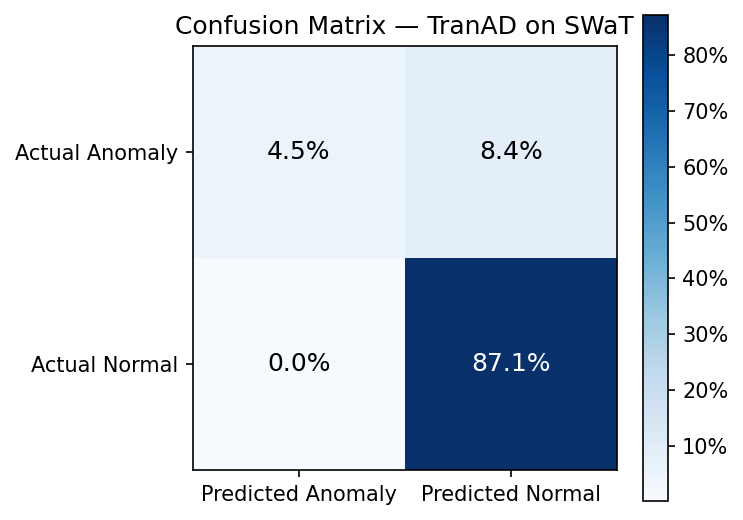
\includegraphics[width=0.7\textwidth]{confusion_matrix_TranAD_SWaT.png}
    \caption{Confusion matrix for TranAD on SWaT. Rows represent the 
    actual class and columns the predicted class.}
    \label{fig:cm_tranad_swat}
\end{figure}


\subsubsection{PR Curve Analysis on PSM}

Figure~\ref{fig:pr_all_psm} shows the precision-recall curves for all five models
on the PSM dataset, included to contextualise the SWaT findings and verify that
the near-random AU-PR behaviour observed there is not a universal property of these
models. In contrast to SWaT, where four of the five models collapsed towards or
below the no-skill baseline almost immediately, all five models remain above the
27.8\% baseline across the full recall range on PSM. TranAD \citep{tranad2022}
again achieves the highest AU-PR (AP = 0.460), but the margin over the remaining
models is substantially smaller than on SWaT, with TimesNet (AP = 0.378),
ModernTCN (AP = 0.383), GTA (AP = 0.304), and Anomaly Transformer (AP = 0.288)
all maintaining meaningful discriminative signal above chance.

\begin{figure}[H]
    \centering
    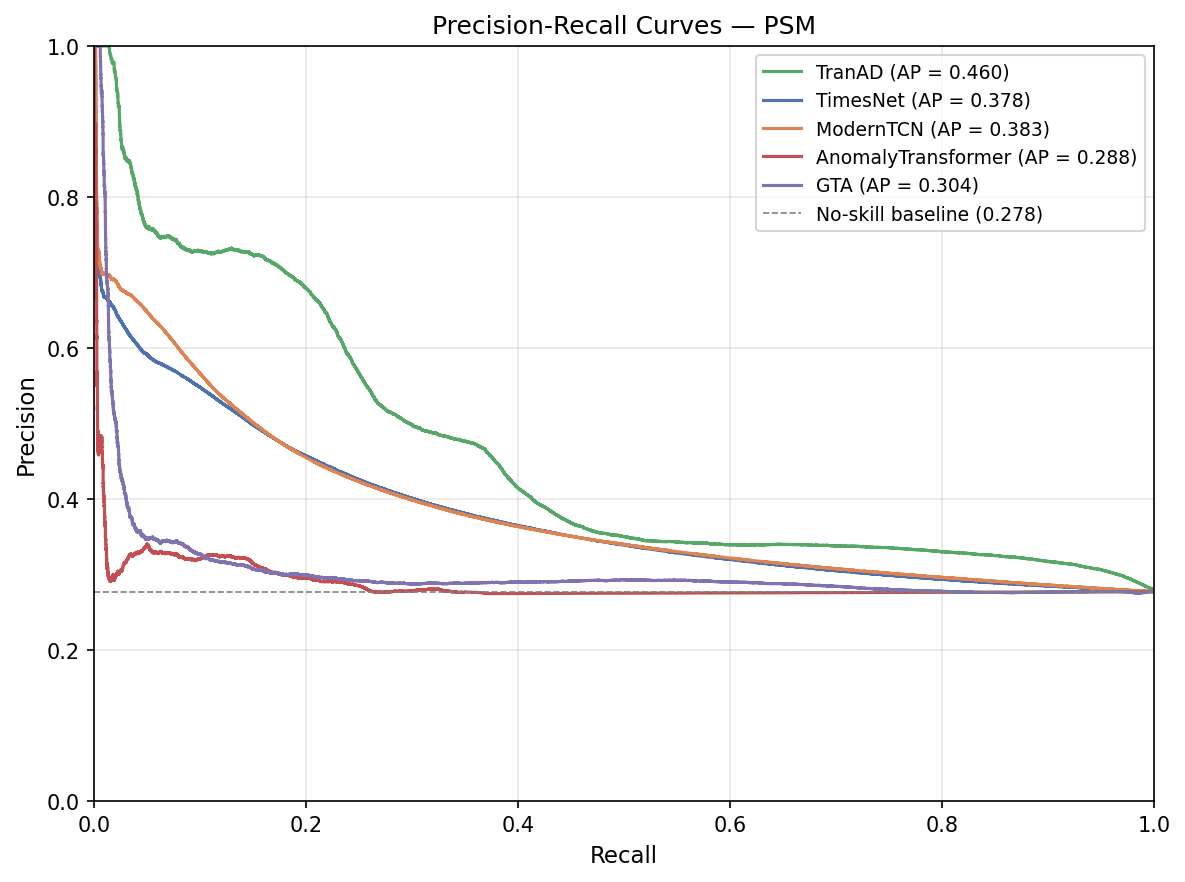
\includegraphics[width=\textwidth]{pr_curves_all_PSM.png}
    \caption{Precision-recall curves for all five models on PSM. The dashed line
    indicates the no-skill baseline equal to the dataset's anomaly rate (27.8\%).}
    \label{fig:pr_all_psm}
\end{figure}

\subsubsection{Missed Detections on SMAP}

On the SMAP dataset, the two CNN-based models perform considerably worse than 
the transformer-based models, with TimesNet achieving an F1 of 68.47\% and ModernTCN 
67.46\%, compared to Anomaly Transformer's 96.41\% which achieved the highest score. 
As shown in Table~\ref{tab:accuracy}, the primary driver of this gap is recall: TimesNet 
and ModernTCN achieve only 55.44\% and 53.85\% respectively, indicating that 
both models miss roughly half of all true anomaly segments. To illustrate 
concretely where this difference originates, Figure~\ref{fig:smap_cnn_recon}, and \ref{fig:smap_anomalytransformer_recon} show 
the same stretch of the SMAP test set (global timesteps 371,000--393,000) for all 
three models. This segment contains five consecutive ground truth anomaly windows 
(orange) that are missed entirely by both CNN-based models but successfully 
detected by Anomaly Transformer.

\begin{figure}[p]
    \centering
    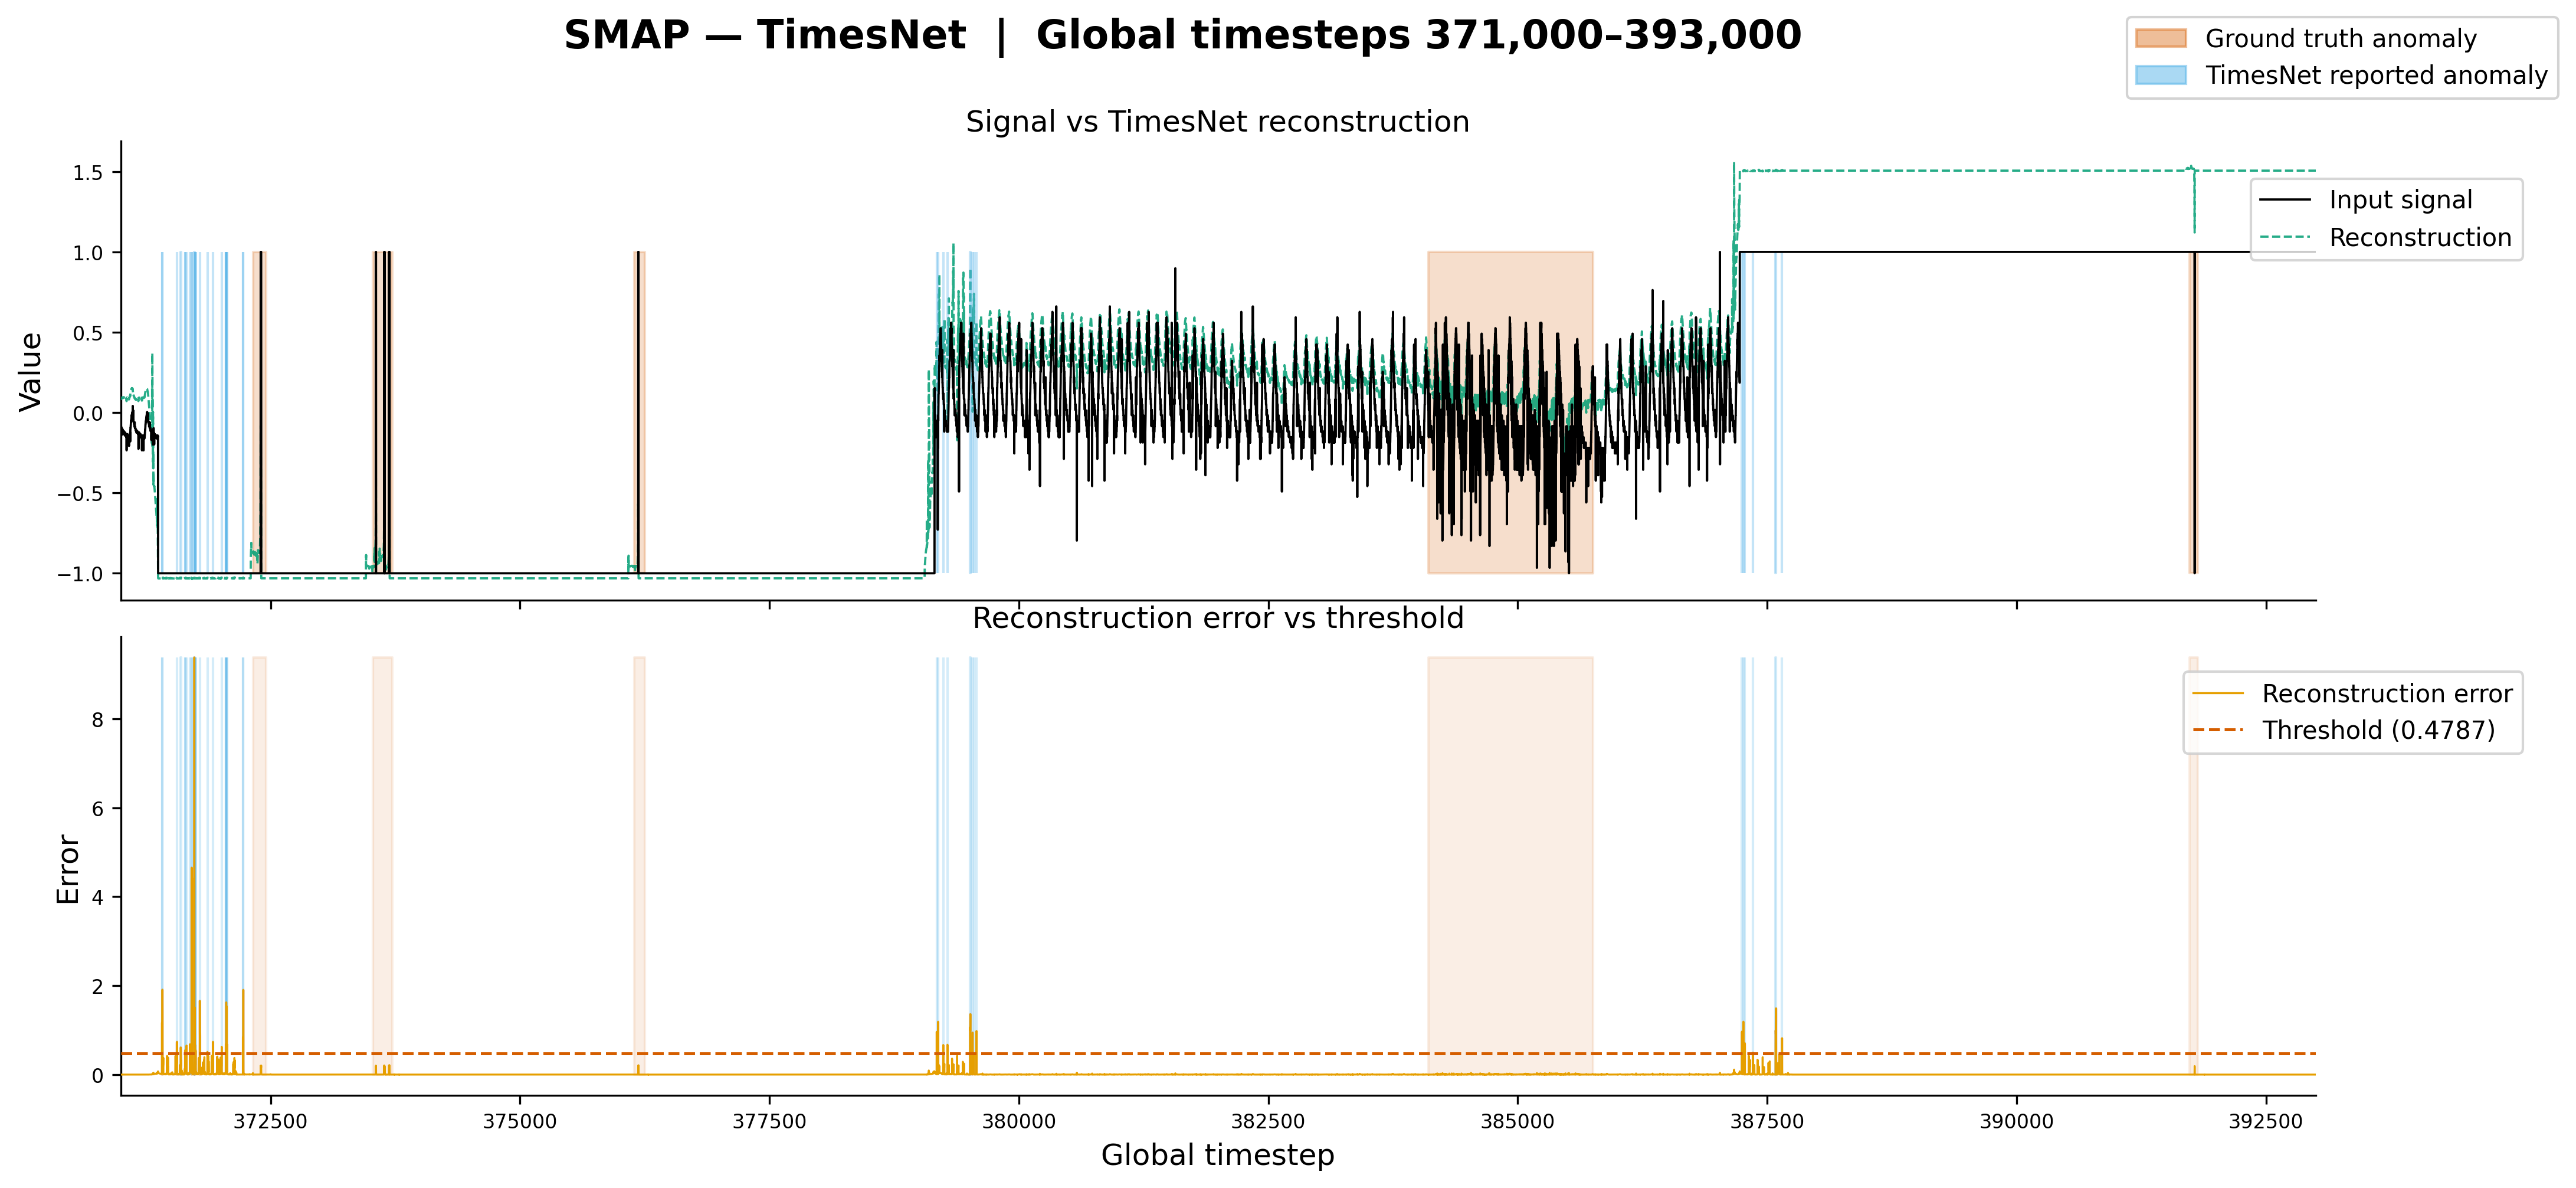
\includegraphics[width=\textwidth]{smap_timesnet_signal_recon.png}
    \vspace{0.5em}
    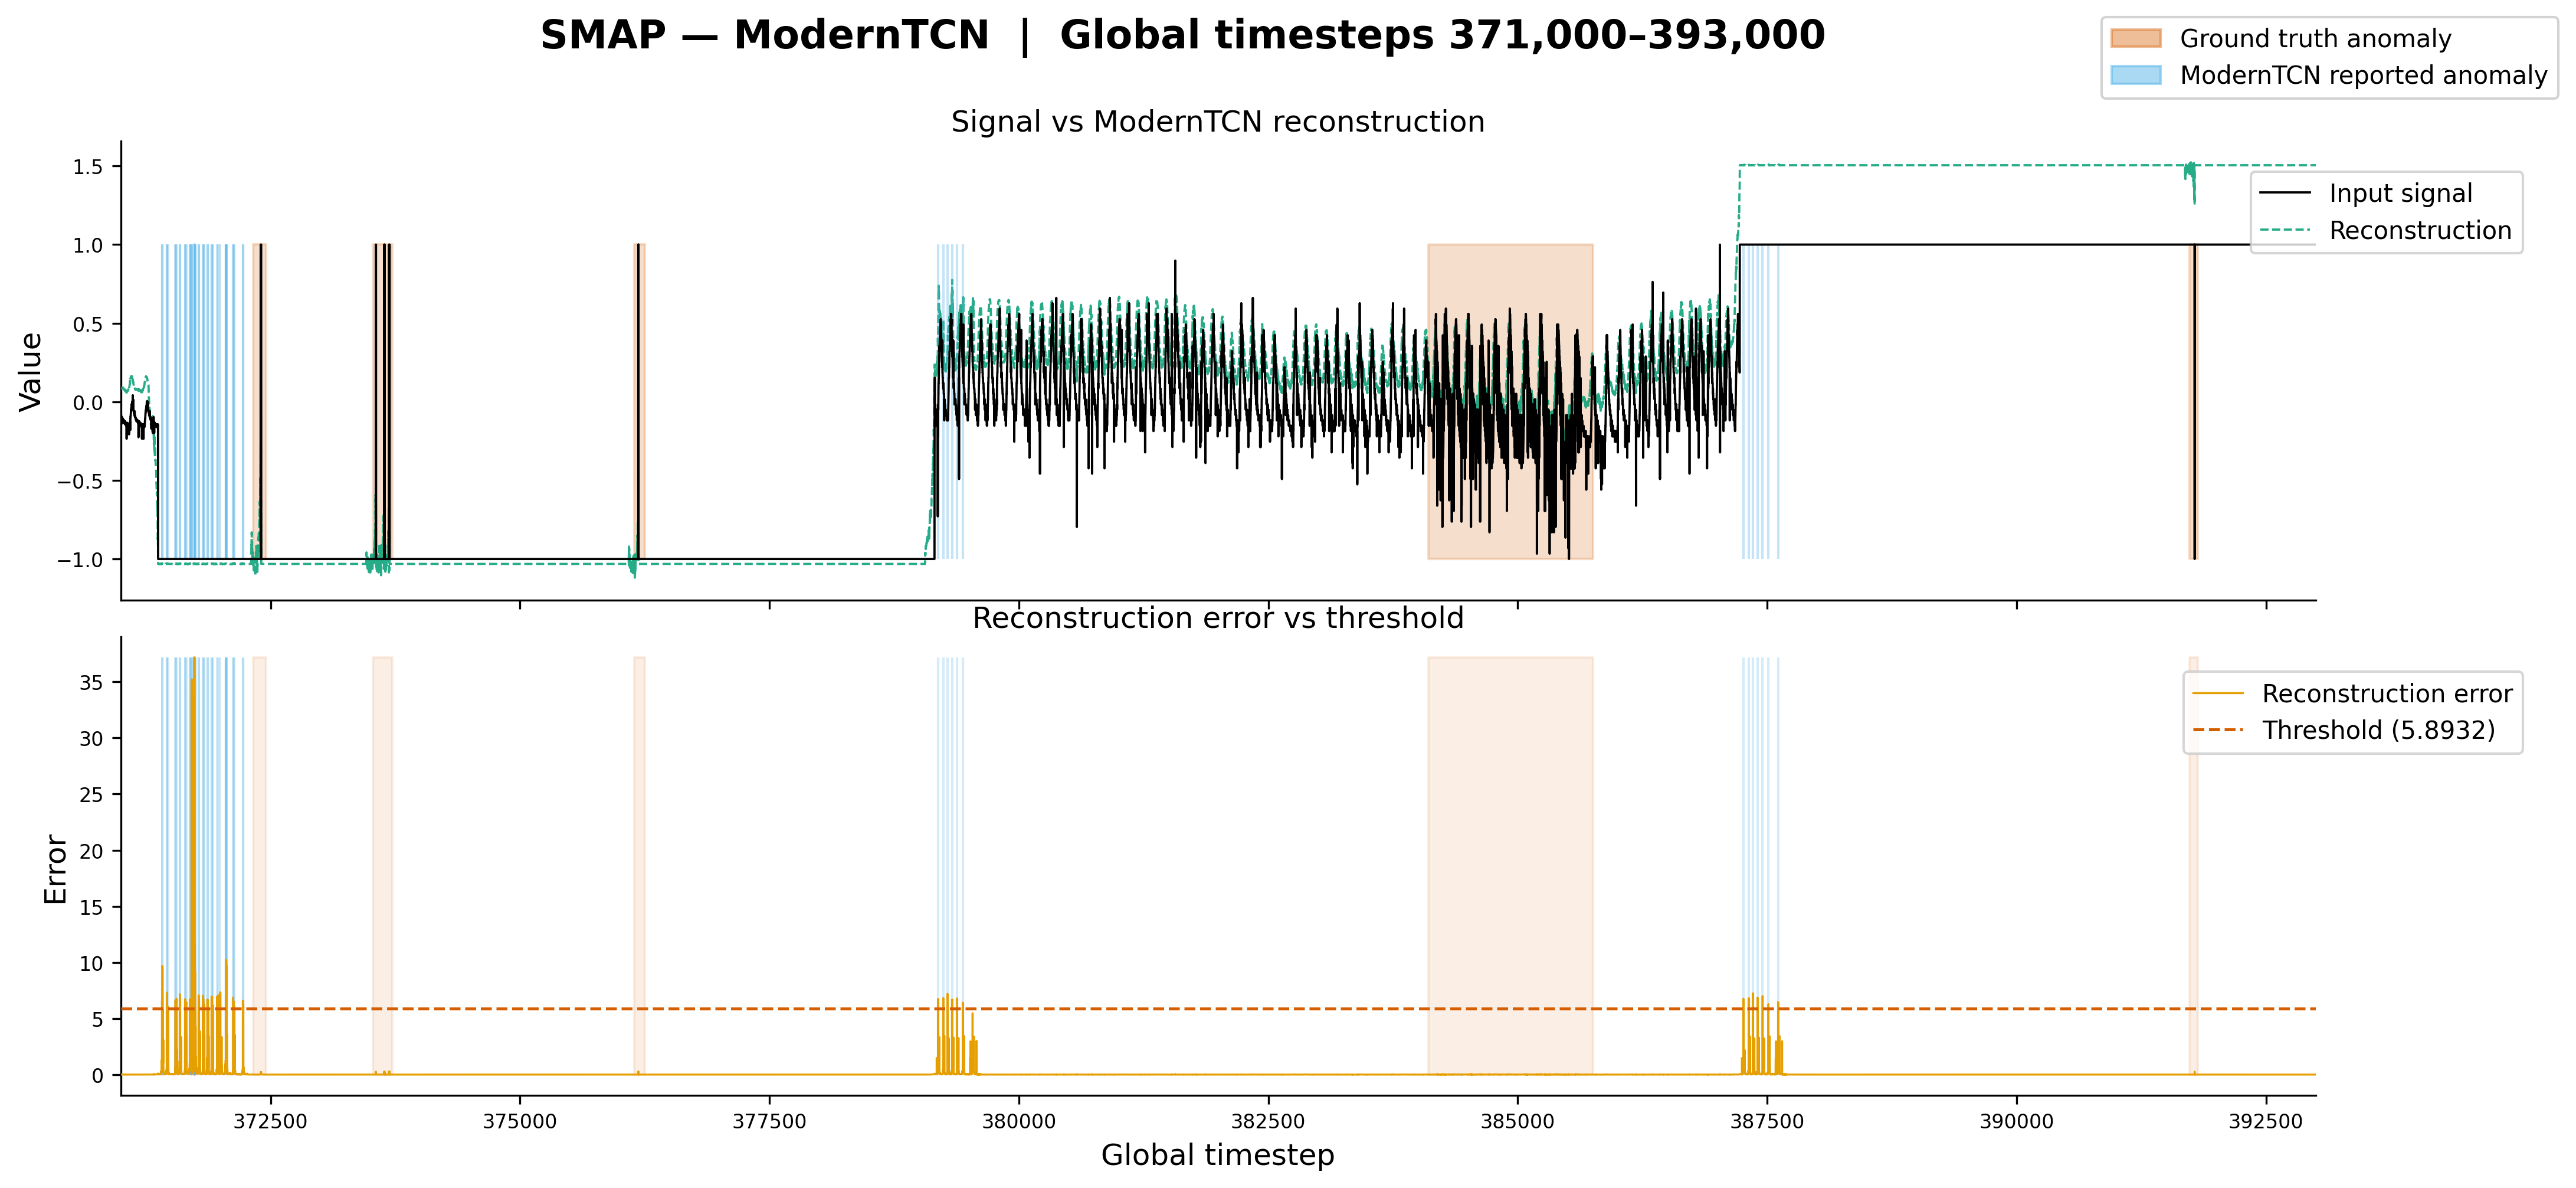
\includegraphics[width=\textwidth]{smap_moderntcn_signal_recon.png}
    \caption{Reconstruction error visualisation for TimesNet (top) and ModernTCN 
    (bottom) on SMAP. For each model, the 
    two panels show: the input signal versus the model reconstruction (dashed green); 
    and the per-timestep reconstruction error aggregated across all 25 channels 
    versus the decision threshold (dashed orange). Blue shading indicates 
    timesteps flagged as anomalous by each model.}
    \label{fig:smap_cnn_recon}
\end{figure}

\begin{figure}[ht]
    \centering
    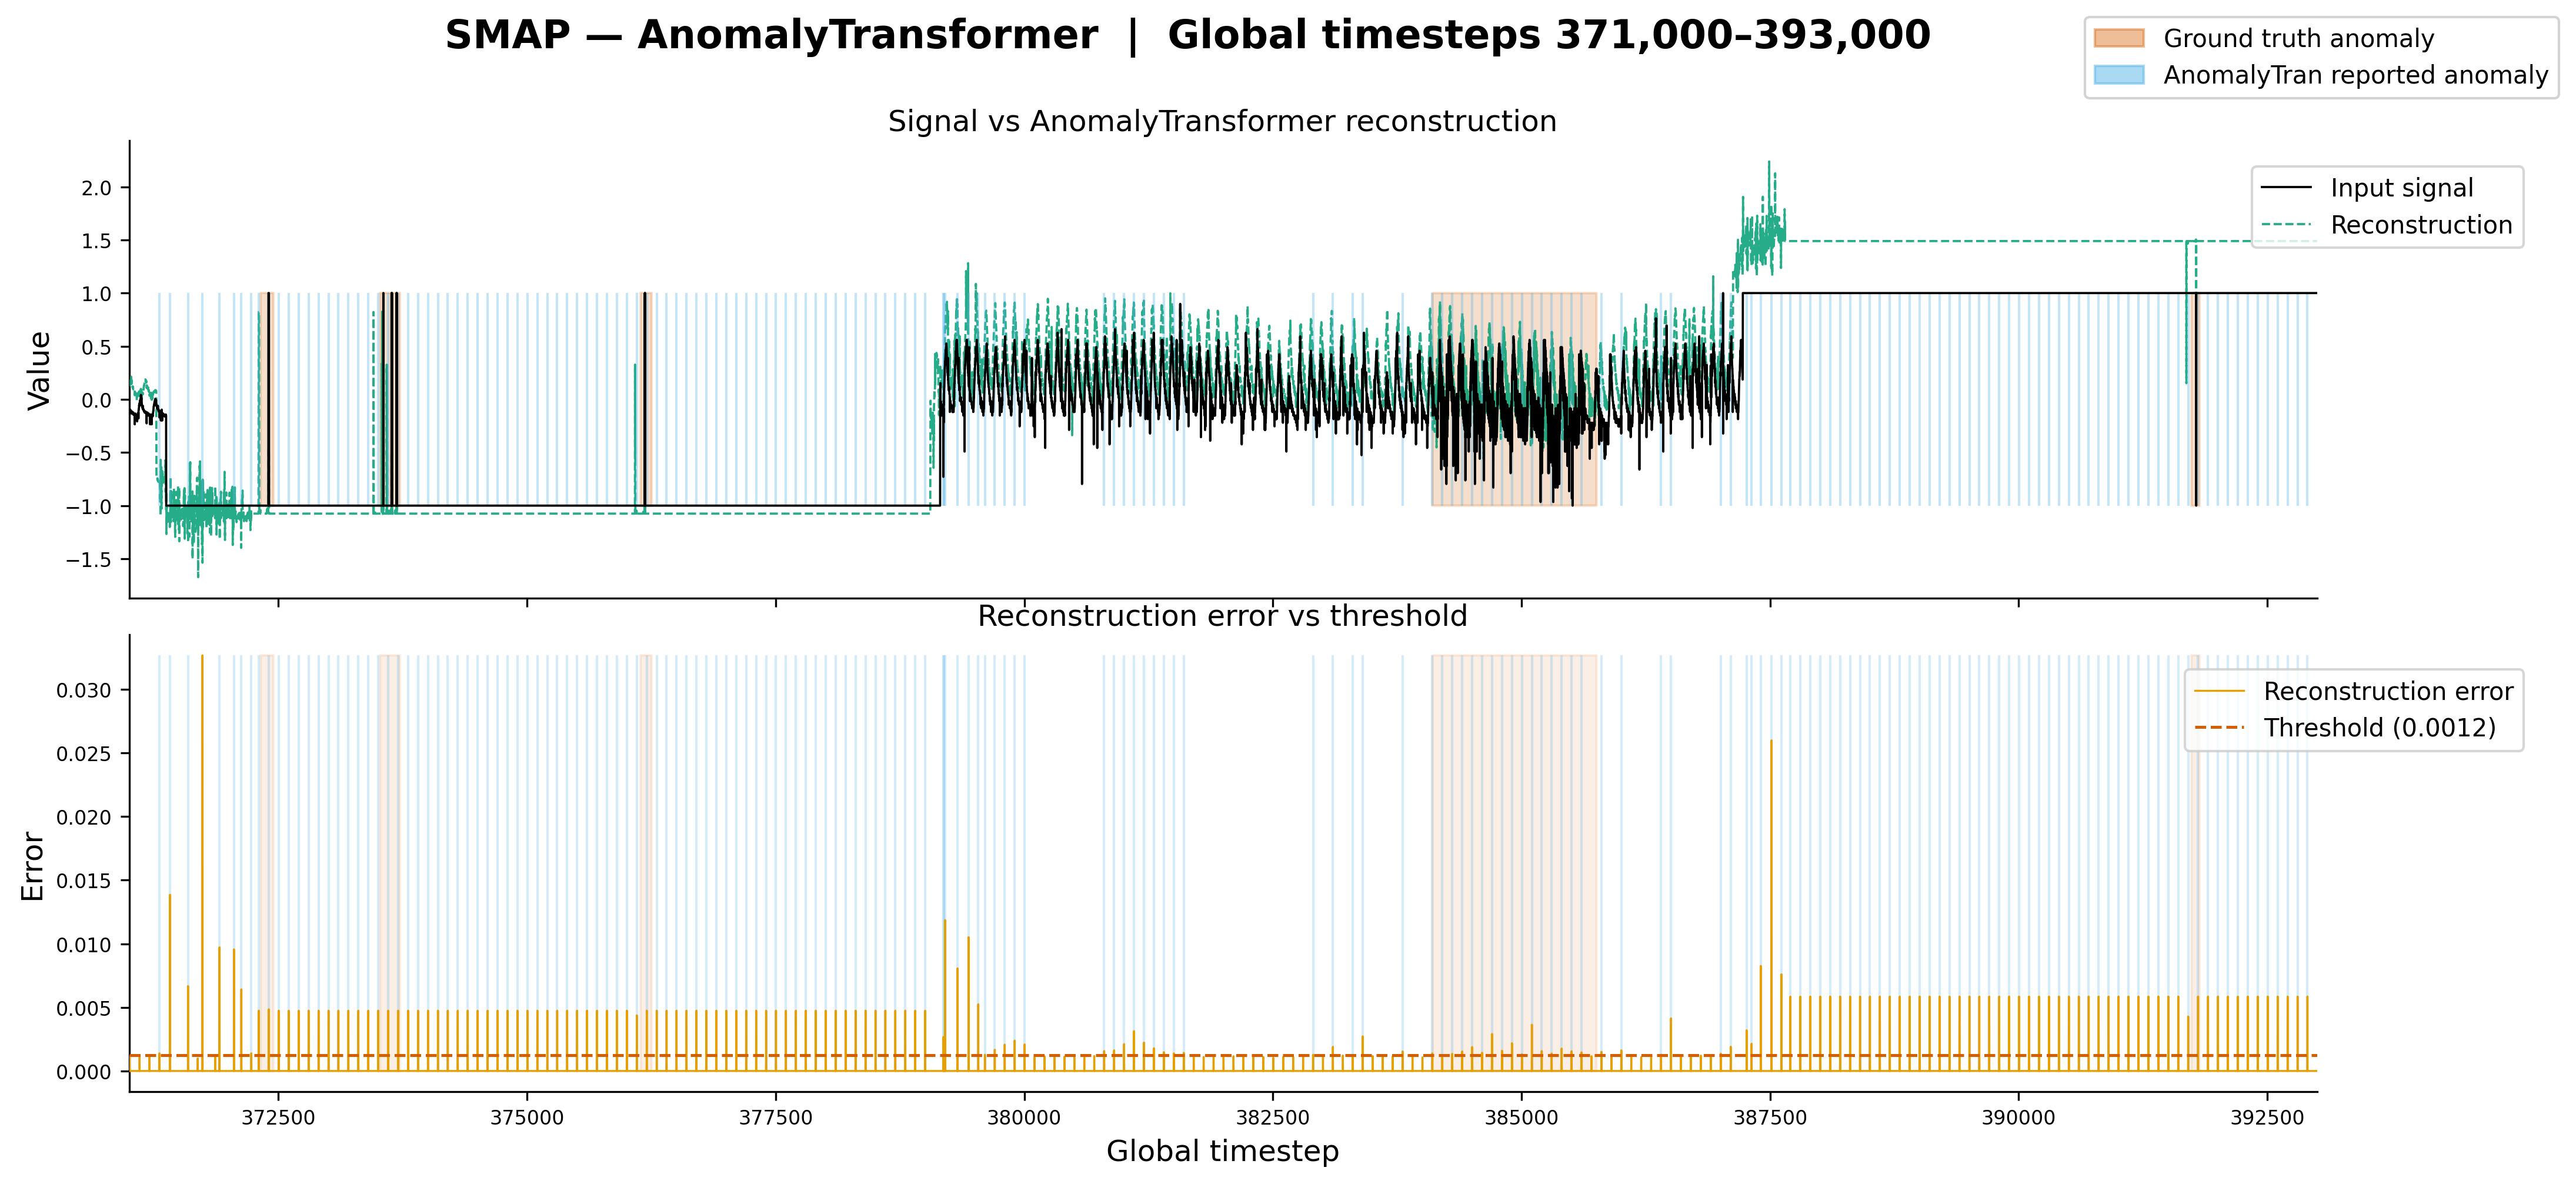
\includegraphics[width=\textwidth]{smap_anomalytransformer_signal_recon.png}
    \caption{Anomaly Transformer on SMAP. 
    The two panels show: the input signal versus the reconstruction (dashed green); and 
    the per-timestep anomaly score --- combining reconstruction error and 
    association discrepancy --- versus the decision threshold 
    (dashed orange). Blue shading indicates timesteps flagged as anomalous.}
    \label{fig:smap_anomalytransformer_recon}
\end{figure}

\paragraph{Anomaly scoring and threshold.}
All three models are trained on normal data only using MSE as the training loss, 
and all three follow the same threshold protocol: $\delta$ is determined to make 
$r = 1\%$ of the validation scores exceed it \citep{anomalytransformer2022}. 
However, their anomaly scores are computed differently.

TimesNet and ModernTCN both use plain reconstruction error as their anomaly 
criterion \citep{timesnet2023, moderntcn2024}. The per-timestep score is the MSE 
between the input and reconstruction averaged across all $d$ channels:

\begin{equation}
    s_t = \frac{1}{d} \sum_{i=1}^{d} \left( x_t^{(i)} - \hat{x}_t^{(i)} \right)^2
    \label{eq:recon_score}
\end{equation}

This yields thresholds of $\delta = 0.4787$ for TimesNet and $\delta = 5.8932$ 
for ModernTCN. The difference in absolute threshold values reflects the different 
internal score scales of the two models, not a difference in strictness, both 
are calibrated to flag the same proportion of validation points.

Anomaly Transformer uses a fundamentally different anomaly score that combines 
reconstruction error with an association discrepancy term 
\citep{anomalytransformer2022}:

\begin{equation}
    \text{AnomalyScore}(\mathcal{X}) = \text{Softmax}(-\text{AssDis}(P, S; 
    \mathcal{X})) \odot \left[\|X_{i,:} - \hat{X}_{i,:}\|_2^2\right]_{i=1,\cdots,N}
    \label{eq:anomaly_transformer_score}
\end{equation}

The association discrepancy measures how differently a time point attends to the 
rest of the series compared to what would be expected under normal conditions. 
Normal points tend to concentrate their attention on temporally adjacent points, 
following a Gaussian prior. Anomalous points, which do not share patterns with 
their neighbours, deviate from this prior, producing a large discrepancy. 
Multiplying this with the reconstruction error means that even when the 
reconstruction error alone is low, the association discrepancy can still elevate 
the anomaly score, giving the model sensitivity to anomalies that a purely 
reconstruction-based approach would miss \citep{anomalytransformer2022}. 
This yields a threshold of $\delta = 0.0012$ for Anomaly Transformer.

\paragraph{Analysis of the visualisations.}
Figure~\ref{fig:smap_cnn_recon} and 
\ref{fig:smap_anomalytransformer_recon} show the input signal, reconstruction, 
and anomaly score relative to the decision threshold for all three models over 
the same segment of the SMAP test set. Note that while the plots display a single 
representative channel, the reconstruction error shown in the bottom panel is 
aggregated across all 25 SMAP channels simultaneously, meaning that the score 
at any given timestep reflects the combined reconstruction quality across the 
entire multivariate signal.

For both TimesNet and ModernTCN, the reconstruction error remains well below 
the threshold throughout the five consecutive ground truth anomaly segments 
(orange), including the large oscillation amplitude change around timesteps 
383,000--386,000. The green dashed reconstruction closely follows the input 
signal during this period, suggesting that both models reconstruct the anomalous 
pattern sufficiently well that it does not produce a detectable increase in MSE. 
Brief threshold crossings are visible at sharp signal transitions, 
but these spikes are narrow and do not correspond 
to the labelled anomaly windows. This is because the spike anomalies are very 
short in duration: even when a few timesteps are poorly reconstructed, their 
contribution to the MSE is averaged over the entire 100-timestep window and 
further diluted across all 25 channels, resulting in an aggregate error that 
does not reliably exceed the threshold.

The Anomaly Transformer plot presents a markedly different picture. The threshold 
of $\delta = 0.0012$ is extremely low relative to the score range, and the 
anomaly score crosses it frequently throughout the segment, producing many short, 
regularly-spaced detections in both normal and anomalous regions. As a result, 
at least one timestep within each of the five ground truth anomaly windows is 
flagged, and under the point-adjust protocol each window is therefore credited 
as fully detected. This behaviour is consistent with the known tendency of 
point-adjusted F1 to overestimate detection performance when a model flags 
anomalies at a high base rate \citep{darban2024carla}, and is reflected in 
Anomaly Transformer's modest AU-PR on SMAP (12.90\%) relative to its F1 
(96.41\%).



\subsection{Memory Usage}

For IoT edge deployment, memory is often the 
binding constraint: microcontrollers and low-power embedded processors typically operate under 
RAM budgets of a few megabytes, and a model that fits comfortably on a server-grade GPU may 
be entirely impractical on constrained hardware \citep{wang2025optimizing}. The five memory 
metrics introduced in Section~\ref{subsec:memory} --- parameter count, exact weight memory, 
GPU-allocated weight memory, peak training memory, and peak inference memory --- capture 
different aspects of this footprint, from the minimum cost of storing a trained model to the 
maximum memory demand placed on the device during a forward pass.

To investigate whether these footprints translate into genuine deployment constraints, 
experiments were conducted in two distinct hardware environments. The first is a standard 
server setup equipped with a GPU, representative of the training and development environment 
in which all five models were originally designed and evaluated. The second is a resource-constrained 
edge device, representative of the target deployment scenario considered throughout this thesis. 
Comparing memory usage across these two environments reveals not only how the absolute footprints 
differ between architectures, but also whether a model's memory demand is feasible in the 
setting where anomaly detection is ultimately intended to run.

An important distinction is made between training and inference memory throughout this section. 
As described in Section~\ref{subsec:memory}, peak training memory includes the full 
computational graph retained by PyTorch for backpropagation, while peak inference memory 
reflects only what is needed during a forward pass. Since edge deployment involves inference 
only the 
peak inference memory and the exact weight memory are the operationally relevant figures for 
assessing deployability. Peak training memory is reported as a complementary indicator of 
the overhead imposed by the computation graph, which is relevant when evaluating whether a 
model could realistically be fine-tuned or retrained on-device in the future.

An important methodological difference must be noted 
for TranAD. Inspection of the original codebase reveals that TranAD's training and inference 
routines hardcode execution to the CPU via explicit \texttt{.cpu()} calls, meaning the model 
never utilises a GPU even when one is available \citep{tranad2022}. As a consequence, 
\textit{all} memory figures reported for 
TranAD in Tables~\ref{tab:memory_static_server} and~\ref{tab:memory_runtime_server} reflect 
CPU RAM rather than GPU VRAM: this applies not only to the runtime metrics --- peak training 
memory, peak inference memory, and overhead --- but also to the allocated weight memory 
(W\textsubscript{alloc}), which is measured from the CPU memory allocator rather than 
PyTorch's GPU memory tracker used for all other models. The exact weight memory 
(W\textsubscript{ex}), computed analytically as parameter count multiplied by bytes per 
element, is hardware-independent and comparable across models.

TranAD and GTA both operate 
in \texttt{float64} (double precision) at runtime, meaning each parameter occupies 
8\,bytes rather than the 4\,bytes of \texttt{float32}. The exact weight memory 
(W\textsubscript{ex}) is therefore computed as parameter count $\times$ 8\,B for TranAD 
and GTA, and parameter count $\times$ 4\,B for TimesNet, ModernTCN, and Anomaly Transformer. 
This must be taken into account when comparing parameter counts to weight memory across 
models: a model with fewer parameters can nonetheless have a larger storage footprint if it 
operates in double precision.

\subsubsection{Static Memory Footprint}
\label{subsubsec:static_memory}

\begin{table}[ht]
\centering
\caption{Static memory footprint per model across five benchmark datasets (server environment).
\textit{Params} is the total parameter count;
W\textsubscript{ex} = exact weight memory, computed as params $\times$ 4\,B for 
TimesNet, ModernTCN, and Anomaly Transformer (\texttt{float32}), and params $\times$ 8\,B 
for TranAD$^\dagger$ and GTA (\texttt{float64});
W\textsubscript{alloc} = allocated weight memory, measured from GPU VRAM for all models 
except TranAD$^\dagger$, for which it reflects CPU RAM.
All memory values in MB.
Lowest value per row in \textbf{bold}, second-lowest \underline{underlined}.}
\label{tab:memory_static_server}
\begin{tabular}{ll rrrrr}
\toprule
\textbf{Dataset} & \textbf{Metric} $\downarrow$
    & \thead{\textbf{TimesNet}\\\citep{timesnet2023}}
    & \thead{\textbf{ModTCN}\\\citep{moderntcn2024}}
    & \thead{\textbf{TranAD}$^\dagger$\\\citep{tranad2022}}
    & \thead{\textbf{AnomTr.}\\\citep{anomalytransformer2022}}
    & \thead{\textbf{GTA}\\\citep{gta2022}} \\
\midrule
\multirow{3}{*}{SMD}
    & Params             & 7{,}041{,}190 & \underline{653{,}000} & \textbf{127{,}538} & 4{,}828{,}222 & 797{,}450 \\
    & W\textsubscript{ex}  &  28.16 & \underline{2.61} & \textbf{1.02} & 18.42 &  6.08 \\
    & W\textsubscript{alloc}$^\dagger$ &  30.44 & \underline{2.65} & \textbf{1.03} & 28.77 & 15.88 \\
\midrule
\multirow{3}{*}{MSL}
    & Params             & 7{,}045{,}559 & 1{,}064{,}264 & \textbf{261{,}243} & 4{,}863{,}055 & \underline{844{,}523} \\
    & W\textsubscript{ex}  &  28.28 & \underline{4.26} & \textbf{2.09} & 18.55 &  6.44 \\
    & W\textsubscript{alloc}$^\dagger$ &  30.46 & \underline{4.32} & \textbf{2.10} & 28.90 & 16.26 \\
\midrule
\multirow{3}{*}{SMAP}
    & Params             & 1{,}761{,}753 & \underline{143{,}01} & \textbf{57{,}273} & 4{,}801{,}585 & 769{,}253 \\
    & W\textsubscript{ex}  & 7.05 &  \underline{0.57} & \textbf{0.46} & 18.32 &  5.87 \\
    & W\textsubscript{alloc}$^\dagger$ &  7.70 &  \underline{0.59} & \textbf{0.46} & 28.67 & 15.66 \\
\midrule
\multirow{3}{*}{SWaT}
    & Params             & 7{,}044{,}531 & 960{,}840 & \textbf{225{,}519} & 4{,}854{,}859 & \underline{832{,}407} \\
    & W\textsubscript{ex}  &  28.18 & \underline{3.84} & \textbf{1.80} & 18.52 &  6.35 \\
    & W\textsubscript{alloc}$^\dagger$ &  30.45 & \underline{3.90} & \textbf{1.81} & 28.87 & 16.16 \\
\midrule
\multirow{3}{*}{PSM}
    & Params             & 1{,}761{,}753 & \underline{143{,}016} & \textbf{57{,}273} & 4{,}801{,}585 & 769{,}253 \\
    & W\textsubscript{ex}  &  7.05 &  \underline{0.57} & \textbf{0.46} & 18.32 &  5.87 \\
    & W\textsubscript{alloc}$^\dagger$ &  7.70 &  \underline{0.59} & \textbf{0.46} & 28.67 & 15.66 \\
\midrule
\multirow{3}{*}{Average}
    & Params             & 4{,}930{,}957 & \underline{592{,}827} & \textbf{145{,}769} & 4{,}829{,}861 & 802{,}577 \\
    & W\textsubscript{ex}  &  19.74 & \underline{2.37} & \textbf{1.17} & 18.43 &  6.12 \\
    & W\textsubscript{alloc}$^\dagger$ &  21.35 & \underline{2.41} & \textbf{1.17} & 28.78 & 15.92 \\
\bottomrule
\multicolumn{7}{l}{\footnotesize $^\dagger$ TranAD executes on CPU; W\textsubscript{alloc} reflects CPU-allocated weight memory for TranAD,}\\
\multicolumn{7}{l}{\footnotesize \phantom{$^\dagger$} GPU-allocated weight memory for all other models.}
\end{tabular}
\end{table}

Table~\ref{tab:memory_static_server} reveals a clear separation between models in terms 
of static memory footprint. TranAD \citep{tranad2022} is the most parameter-efficient 
model across all datasets, with an average of 145{,}769 parameters and an exact weight 
memory of just 1.17\,MB --- more than an order of magnitude smaller than any other model. 
At the opposite extreme, TimesNet \citep{timesnet2023} and Anomaly Transformer 
\citep{anomalytransformer2022} are the heaviest models, with average parameter counts of 
approximately 4.9M and 4.8M respectively, translating to exact weight memories of 19.74\,MB 
and 18.43\,MB. ModernTCN \citep{moderntcn2024} is the second lightest model with an average of 
592{,}827 parameters and 2.37\,MB, closely behind TranAD. GTA \citep{gta2022} sits 
in the middle of the ranking at 6.12\,MB on average, with its \texttt{float64} precision 
resulting in a higher storage cost than its parameter count alone would suggest. 

The allocated weight memory (W\textsubscript{alloc}) closely tracks W\textsubscript{ex} 
for TranAD, TimesNet, and ModernTCN, with small differences attributable to PyTorch's 
block-based memory allocator and persistent buffers. GTA and Anomaly Transformer both 
show a consistent gap of approximately 10\,MB between W\textsubscript{ex} and 
W\textsubscript{alloc} across all datasets. For GTA, this gap is particularly striking 
in relative terms --- W\textsubscript{alloc} is roughly 2.6$\times$ larger than 
W\textsubscript{ex} --- suggesting that GTA's architecture retains a substantial amount 
of non-parameter state, such as the learned adjacency matrix used for graph structure 
learning \citep{gta2022}, that is allocated as part of the model but does not contribute 
to the parameter count. For Anomaly Transformer the relative gap is smaller (roughly 
1.6$\times$), but the absolute difference is the same, pointing to a similar phenomenon 
of persistent architecture-specific buffers beyond the learnable weights.

From a pure storage perspective, TranAD and ModernTCN are the strongest candidates for 
edge deployment: both fit well within the RAM constraints of low-power embedded devices, 
with TranAD's 1.17\,MB and ModernTCN's 2.37\,MB sitting comfortably below the memory 
budgets of even relatively constrained hardware. TimesNet and Anomaly Transformer, at 
roughly 21--28\,MB depending on the dataset, remain feasible on more capable edge 
platforms. GTA's inflated W\textsubscript{alloc} of approximately 
16\,MB makes it heavier than its parameter count alone would suggest, which is a relevant 
consideration when estimating its true storage cost on a constrained device.

As shown in Figure~\ref{fig:memory_alloc_variability}, TimesNet \citep{timesnet2023} 
exhibits by far the highest variability in allocated weight memory across datasets, 
with its dots spanning from 7.70\,MB on SMAP and PSM to 30.46\,MB on SMD, MSL, and SWaT. 
All other models show comparatively tight clustering: 
Anomaly Transformer's dots are nearly indistinguishable at 28.67--28.90\,MB, GTA 
spans 15.66--16.26\,MB. While TranAD and ModernTCN do vary across datasets, their spread 
is proportionally small.

This variability in TimesNet is not a random artefact but a direct consequence of 
an explicit architectural design choice. TimesNet sets its internal hidden dimension 
$d_\text{model}$ as a function of the input dimensionality $C$:
\begin{equation}
    d_\text{model} = \min\!\left\{\max\!\left\{2^{\lceil \log C \rceil},\, 
    d_\text{min}\right\},\, d_\text{max}\right\}
    \label{eq:timesnet_dmodel}
\end{equation}
where $d_\text{min} = 32$ and $d_\text{max} = 128$ for anomaly detection 
\citep{timesnet2023}. Among the five benchmark datasets, SMAP and PSM both have 
25 dimensions, mapping to $d_\text{model} = 32$, while SMD (38), MSL (55), and 
SWaT (51) all map to $d_\text{model} = 64$. The hidden dimension $d_\text{model}$ 
controls the width of every layer in the network --- that is, how many features 
each layer processes internally. Most weight matrices in a neural network have 
dimensions that are proportional to $d_\text{model}$, so when $d_\text{model}$ 
doubles from 32 to 64, the number of parameters in each such matrix grows by a 
factor of $64^2 / 32^2 = 4$, since both the input and output sides of the matrix 
scale together. This is why halving $d_\text{model}$ reduces the total parameter 
count by approximately four rather than two.


\begin{figure}[ht]
    \centering
    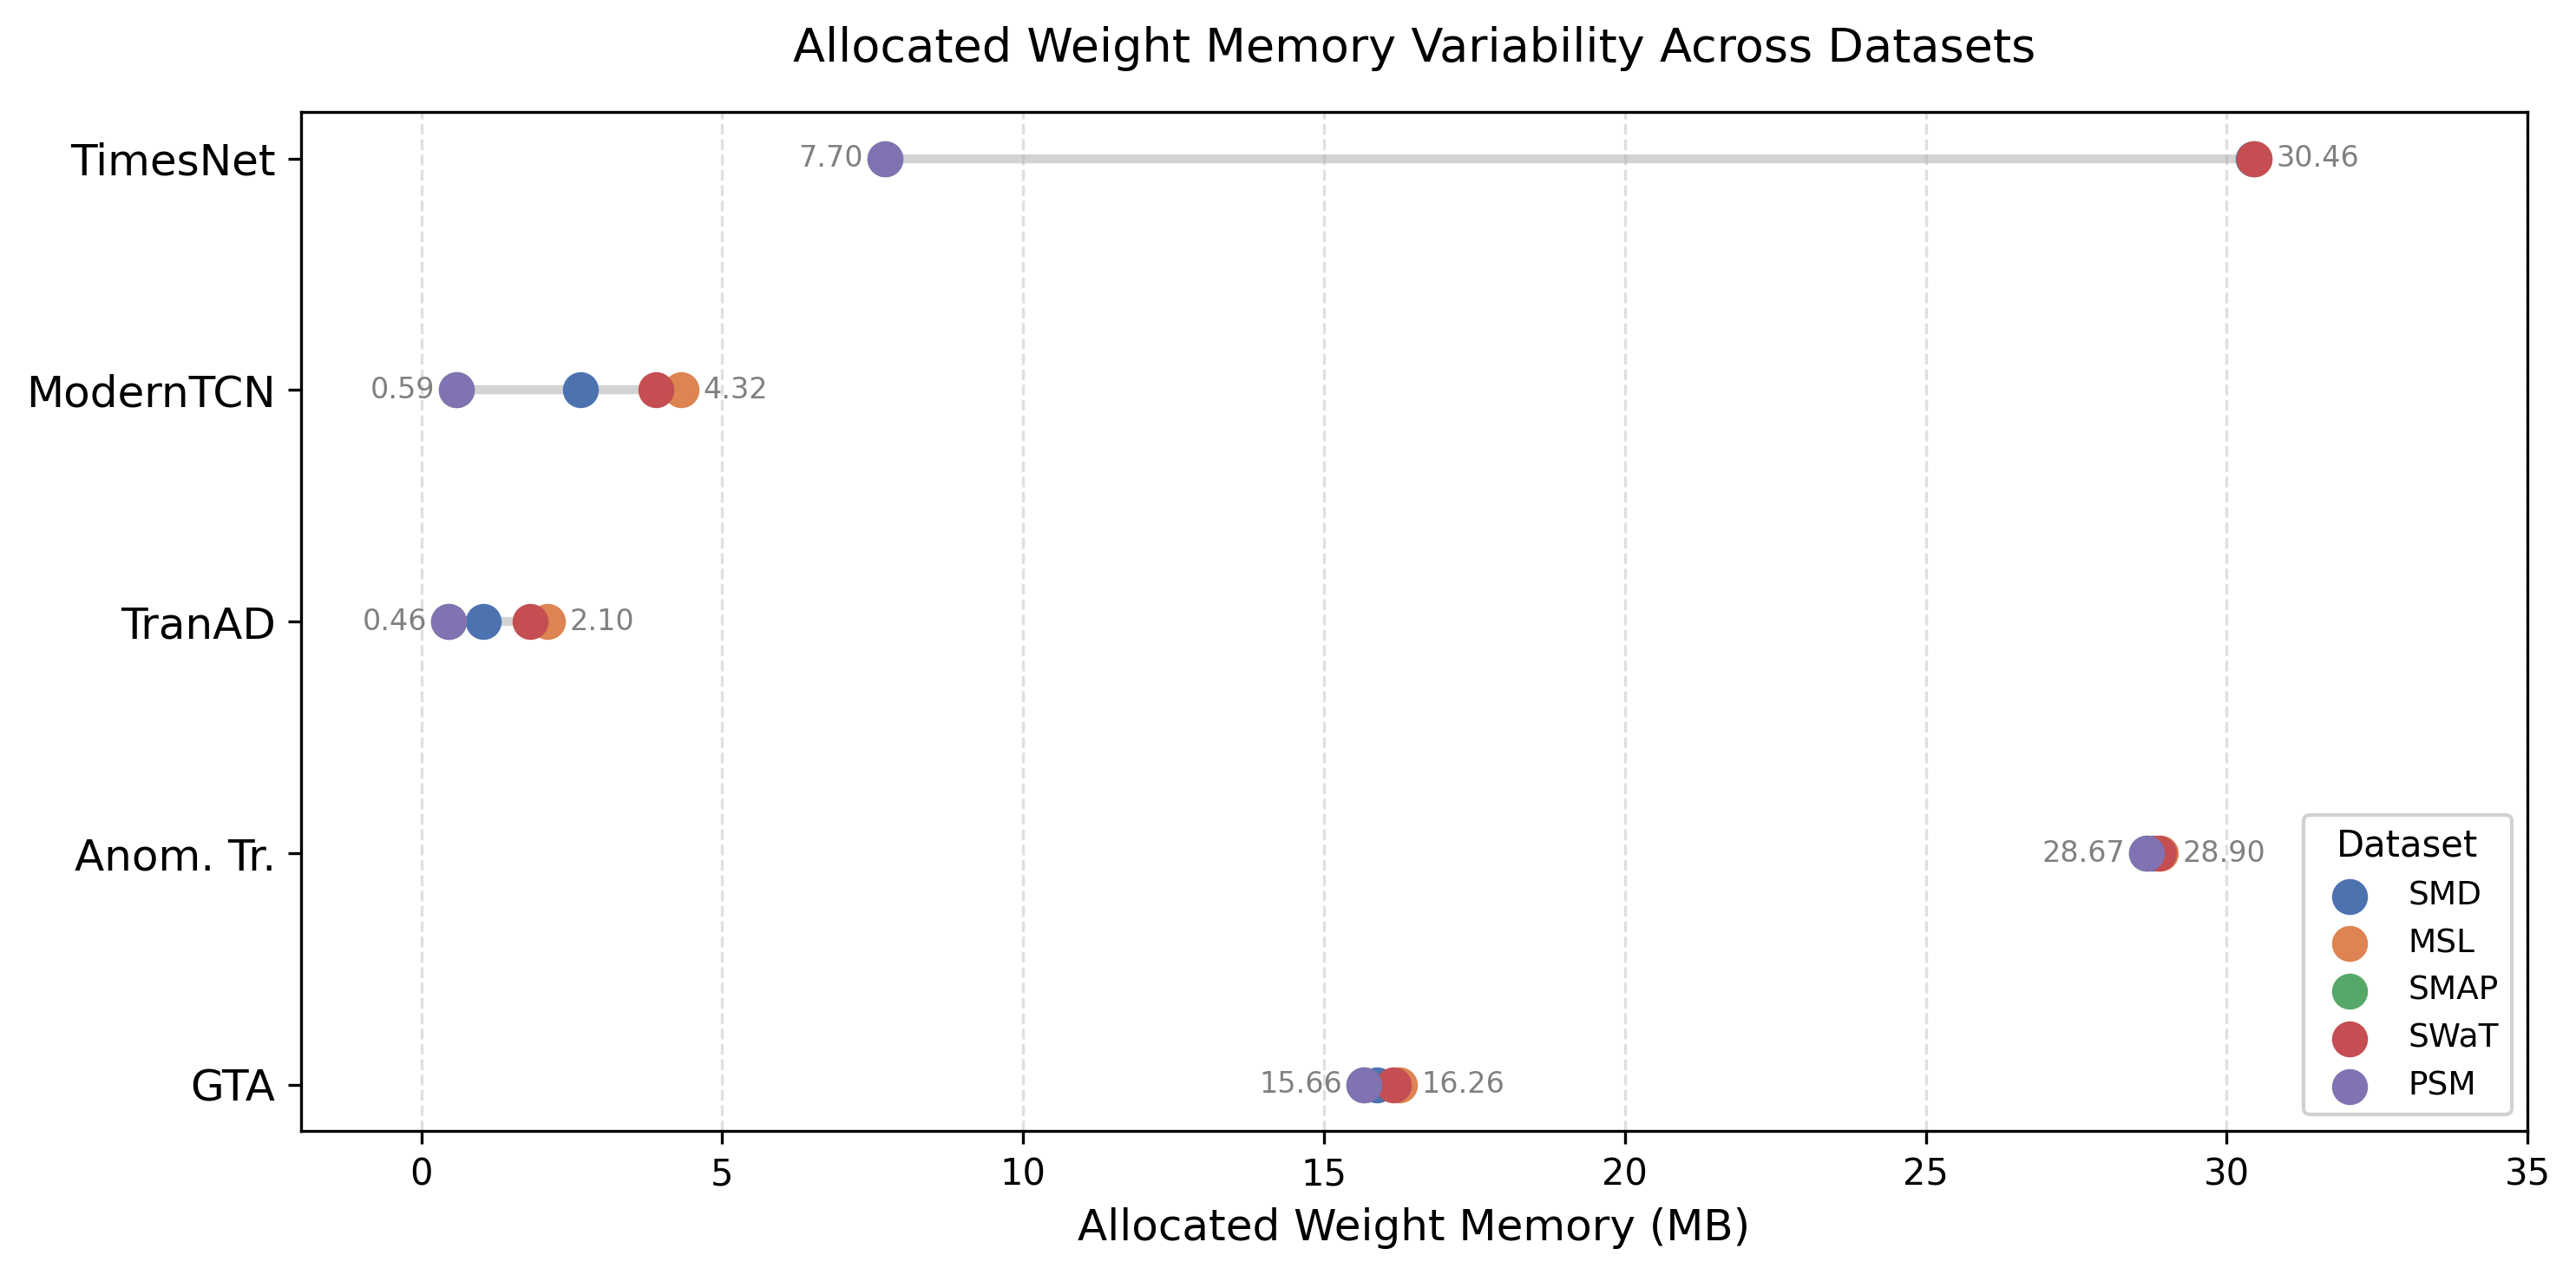
\includegraphics[width=\textwidth]{memory_alloc_variability.png}
    \caption{Allocated weight memory variability across datasets for each model.
    Each dot represents one dataset; the horizontal line spans the min--max range.
    Some dots may not be visible where multiple datasets yield identical or 
    near-identical values, causing them to overlap.}
    \label{fig:memory_alloc_variability}
\end{figure}

The same input-adaptive scaling applies to ModernTCN \citep{moderntcn2024}, which 
uses an identical formula to set its channel number $D$ --- also referred to as the 
dimension of hidden states --- with $d_\text{min} = 8$ and $d_\text{max} = 256$ for 
anomaly detection \citep{moderntcn2024}. This produces the same two-cluster pattern 
visible in Figure~\ref{fig:memory_alloc_variability}: ModernTCN's allocated weight 
memory spans from 0.59\,MB on SMAP and PSM ($D = 32$) to 4.32\,MB on MSL ($D = 64$). 
However, because ModernTCN's architecture relies on 
depthwise and grouped pointwise convolutions rather than the dense 2D inception blocks 
used in TimesNet \citep{timesnet2023}, its absolute weight memory remains substantially 
lower across all datasets --- averaging 2.37\,MB compared to TimesNet's 19.74\,MB. 
This efficiency advantage is directly acknowledged by the ModernTCN authors, who note 
that TimesNet's additional 2D data transformation and aggregation modules introduce 
extra memory overhead and slower training speed, with ModernTCN saving approximately 
57\% of average training time per epoch on anomaly detection benchmarks compared to 
TimesNet \citep{moderntcn2024}. The allocated weight memory results in 
Table~\ref{tab:memory_static_server} are consistent with this finding: despite sharing 
the same input-adaptive scaling strategy, ModernTCN's parameter-efficient depthwise 
convolution design translates directly into a smaller storage footprint at every 
dataset, making it the more viable candidate for deployment on memory-constrained 
edge devices among the two CNN-based models evaluated in this thesis.

The near-perfect consistency of Anomaly Transformer's allocated weight memory across 
datasets --- spanning only 28.67--28.90\,MB regardless of the input dimensionality --- 
stands in sharp contrast to the behaviour of TimesNet and ModernTCN, and 
is a direct consequence of how the model is parameterised. The Anomaly Transformer uses 
a fixed hidden dimension of $d_\text{model} = 512$ with 
$h = 8$ attention heads for all datasets \citep{anomalytransformer2022}, meaning the 
internal width of the model does not adapt to the number of input dimensions. The input 
dimensionality only influences two small layers: the embedding layer at the entrance, 
which maps the raw $d$-dimensional observations into the fixed 512-dimensional space, 
and the reconstruction head at the exit, which maps back. All the weight-heavy components 
in between --- the query, key, value, and output projection matrices of each attention 
head --- are completely independent of the input 
dimensionality. This explains why the parameter count barely changes across datasets.

Anomaly Transformer's 
W\textsubscript{alloc} of approximately 28--29\,MB substantially exceeds its 
W\textsubscript{ex} of approximately 18\,MB. The gap of roughly 10\,MB is attributable 
to persistent buffers that are part of the model's state but are not learnable parameters: 
most notably the Gaussian kernel prior-association matrix $P^l \in \mathbb{R}^{N \times N}$ 
and the series-association matrix $S^l \in \mathbb{R}^{N \times N}$, which are computed 
and retained across the $L = 3$ layers of the Anomaly-Attention mechanism 
\citep{anomalytransformer2022}.
The practical consequence for 
edge deployment is that Anomaly Transformer's memory footprint is both large and 
predictable: it will not shrink on low-dimensional datasets the way TimesNet and 
ModernTCN do, making it fundamentally less adaptable to resource-constrained hardware 
regardless of dimensionality.

GTA's parameter count
varies directly with input dimensionality through the learned
adjacency matrix. GTA's connection learning policy \citep{gta2022} maintains a
per-dataset probability matrix $\Pi \in \mathbb{R}^{M \times M}$, where $M$ is the
number of sensors, to parameterise the Gumbel-Softmax sampling of directed edges among
all sensor pairs. This matrix scales quadratically with the number of input features,
meaning that datasets with more sensors --- such as SMD (38 features) and SWaT
(51 features) --- result in a larger learnable graph structure than lower-dimensional
datasets such as SMAP and PSM (25 features each). 

The substantially larger W\textsubscript{alloc} relative to W\textsubscript{ex} reflects
the fact that the learned adjacency matrix is retained as a persistent non-parameter
buffer at runtime. For GTA, the adjacency matrix constitutes a significant
portion of this allocated state: it is computed and held in memory throughout training
and inference to support the Influence Propagation (IP) convolution, which aggregates
neighbourhood information by propagating differences between sensor embeddings across
the learned graph edges \citep{gta2022}. This buffer is architecture-specific and
persistent --- it is not discarded between forward passes --- which explains why
W\textsubscript{alloc} consistently exceeds W\textsubscript{ex} by a factor of
approximately 2.6$\times$ regardless of dataset.

From a deployment perspective, GTA's average W\textsubscript{alloc} of 15.92\,MB
places it above both TranAD (1.17\,MB) and ModernTCN (2.37\,MB). Unlike TimesNet and
ModernTCN, whose memory footprint shrinks meaningfully on lower-dimensional datasets, 
GTA's reduction is modest:
W\textsubscript{alloc} spans only 15.66--16.26\,MB across the five benchmark datasets.

\subsubsection{Runtime Memory Footprint}
\label{subsubsec:runtime_server}

\begin{table}[ht]
\centering
\caption{Runtime memory footprint per model across five benchmark datasets (server environment), in MB.
Train = peak training memory; Infer = peak inference memory;
OH = overhead (peak training memory $-$ exact weight memory).
TranAD executes on CPU; all other models execute on GPU. 
Lowest value per row in \textbf{bold}, second-lowest \underline{underlined}.}
\label{tab:memory_runtime_server}
\begin{tabular}{ll rrrrr}
\toprule
\textbf{Dataset} & \textbf{Metric} $\downarrow$
    & \thead{\textbf{TimesNet}\\\citep{timesnet2023}}
    & \thead{\textbf{ModTCN}\\\citep{moderntcn2024}}
    & \thead{\textbf{TranAD}$^\dagger$\\\citep{tranad2022}}
    & \thead{\textbf{AnomTr.}\\\citep{anomalytransformer2022}}
    & \thead{\textbf{GTA}\\\citep{gta2022}} \\
\midrule
\multirow{3}{*}{SMD}
    & Train & \underline{408.97} & 470.28 &   \textbf{2.47} & 4228.20 &  777.10 \\
    & Infer & 295.39 & \underline{188.19} &   \textbf{1.45} & 3027.15 &  314.77 \\
    & OH    & \underline{378.53} & 467.62 &   \textbf{1.45} & 4199.43 &  761.22 \\
\midrule
\multirow{3}{*}{MSL}
    & Train & \underline{410.13} & 669.29 &   \textbf{4.81} & 4351.70 & 1178.96 \\
    & Infer & 296.63 & \underline{264.98} &   \textbf{2.72} & 3151.52 &  603.16 \\
    & OH    & \underline{381.07} & 664.96 &   \textbf{1.45} & 4322.79 & 1162.69 \\
\midrule
\multirow{3}{*}{SMAP}
    & Train & 215.64 & \underline{176.75} &   \textbf{1.20} & 4346.71 &  616.12 \\
    & Infer & 104.74 &  \underline{79.37} &   \textbf{0.74} & 3144.19 &  303.65 \\
    & OH    & 207.93 & \underline{176.15} &   \textbf{0.74} & 4318.04 &  600.46 \\
\midrule
\multirow{3}{*}{SWaT}
    & Train & \underline{411.52} & 623.31 &   \textbf{4.19} & 4350.73 & 1019.17 \\
    & Infer & 296.63 & \underline{247.19} &   \textbf{2.39} & 3150.69 &  522.51 \\
    & OH    & \underline{381.07} & 619.41 &   \textbf{0.38} & 4321.86 & 1003.01 \\
\midrule
\multirow{3}{*}{PSM}
    & Train & 212.66 & \underline{176.80} &   \textbf{1.20} & 4346.66 &  617.59 \\
    & Infer & 105.66 &  \underline{79.92} &   \textbf{0.74} & 3144.19 &  304.65 \\
    & OH    & 204.96 & \underline{176.20} &   \textbf{0.74} & 4317.99 &  601.94 \\
\midrule
\multirow{3}{*}{Average}
    & Train & \underline{331.78} & 423.29 &   \textbf{2.77} & 4324.80 &  841.79 \\
    & Infer & 219.81 & \underline{171.93} &   \textbf{1.61} & 3123.55 &  409.75 \\
    & OH    & \underline{310.71} & 420.87 &   \textbf{0.95} & 4296.02 &  825.86 \\
\bottomrule
\multicolumn{7}{l}{\footnotesize $^\dagger$ TranAD executes on CPU; memory measured in RAM rather than GPU VRAM.}
\end{tabular}
\end{table}

Table~\ref{tab:memory_runtime_server} and Figure~\ref{fig:runtime_memory_logscale} 
reveals that Anomaly Transformer's runtime memory
footprint is in a category of its own. At an average peak training memory of 4324.80\,MB
and peak inference memory of 3123.55\,MB it exceeds the lightest GPU-resident model at inference --- ModernTCN at 171.93\,MB --- by
nearly 18$\times$. This stands in sharp contrast to the static footprint analysis, where
Anomaly Transformer's W\textsubscript{alloc} of approximately 28--29\,MB, while the
largest among all models, did not suggest such an extreme runtime demand. The explanation
lies in the quadratic scaling of the attention mechanism with respect to sequence length:
the prior-association matrix $P^l \in \mathbb{R}^{N \times N}$ and series-association
matrix $S^l \in \mathbb{R}^{N \times N}$ must be instantiated and retained across all
$L = 3$ Anomaly-Attention layers during the forward pass \citep{anomalytransformer2022},
producing a high memory demand. For IoT edge deployment, where inference memory is the 
operationally binding
constraint, Anomaly Transformer's runtime footprint renders it infeasible on embedded hardware, 
regardless of dataset or input dimensionality.

At the opposite extreme, TranAD \citep{tranad2022} achieves runtime memory figures that
are remarkable. Its average peak training memory of just
2.77\,MB and peak inference memory of 1.61\,MB are not only the lowest among all five
models by a wide margin, but also nearly indistinguishable from its static weight memory
of 1.17\,MB. The average overhead of 0.95\,MB indicates that TranAD's computational
graph retains almost no intermediate activations during backpropagation. This is
consistent with TranAD's relatively shallow encoder-decoder architecture
\citep{tranad2022}. The practical implication is that TranAD's memory
cost is almost entirely determined by its weights: what fits in storage will also fit
at inference, and the gap between training and deployment is negligible. This property
is particularly valuable in edge scenarios where memory budgets are fixed and
predictable, and where the overhead of maintaining a computational graph --- even
temporarily --- may exceed available capacity.

\begin{figure}[ht]
    \centering
    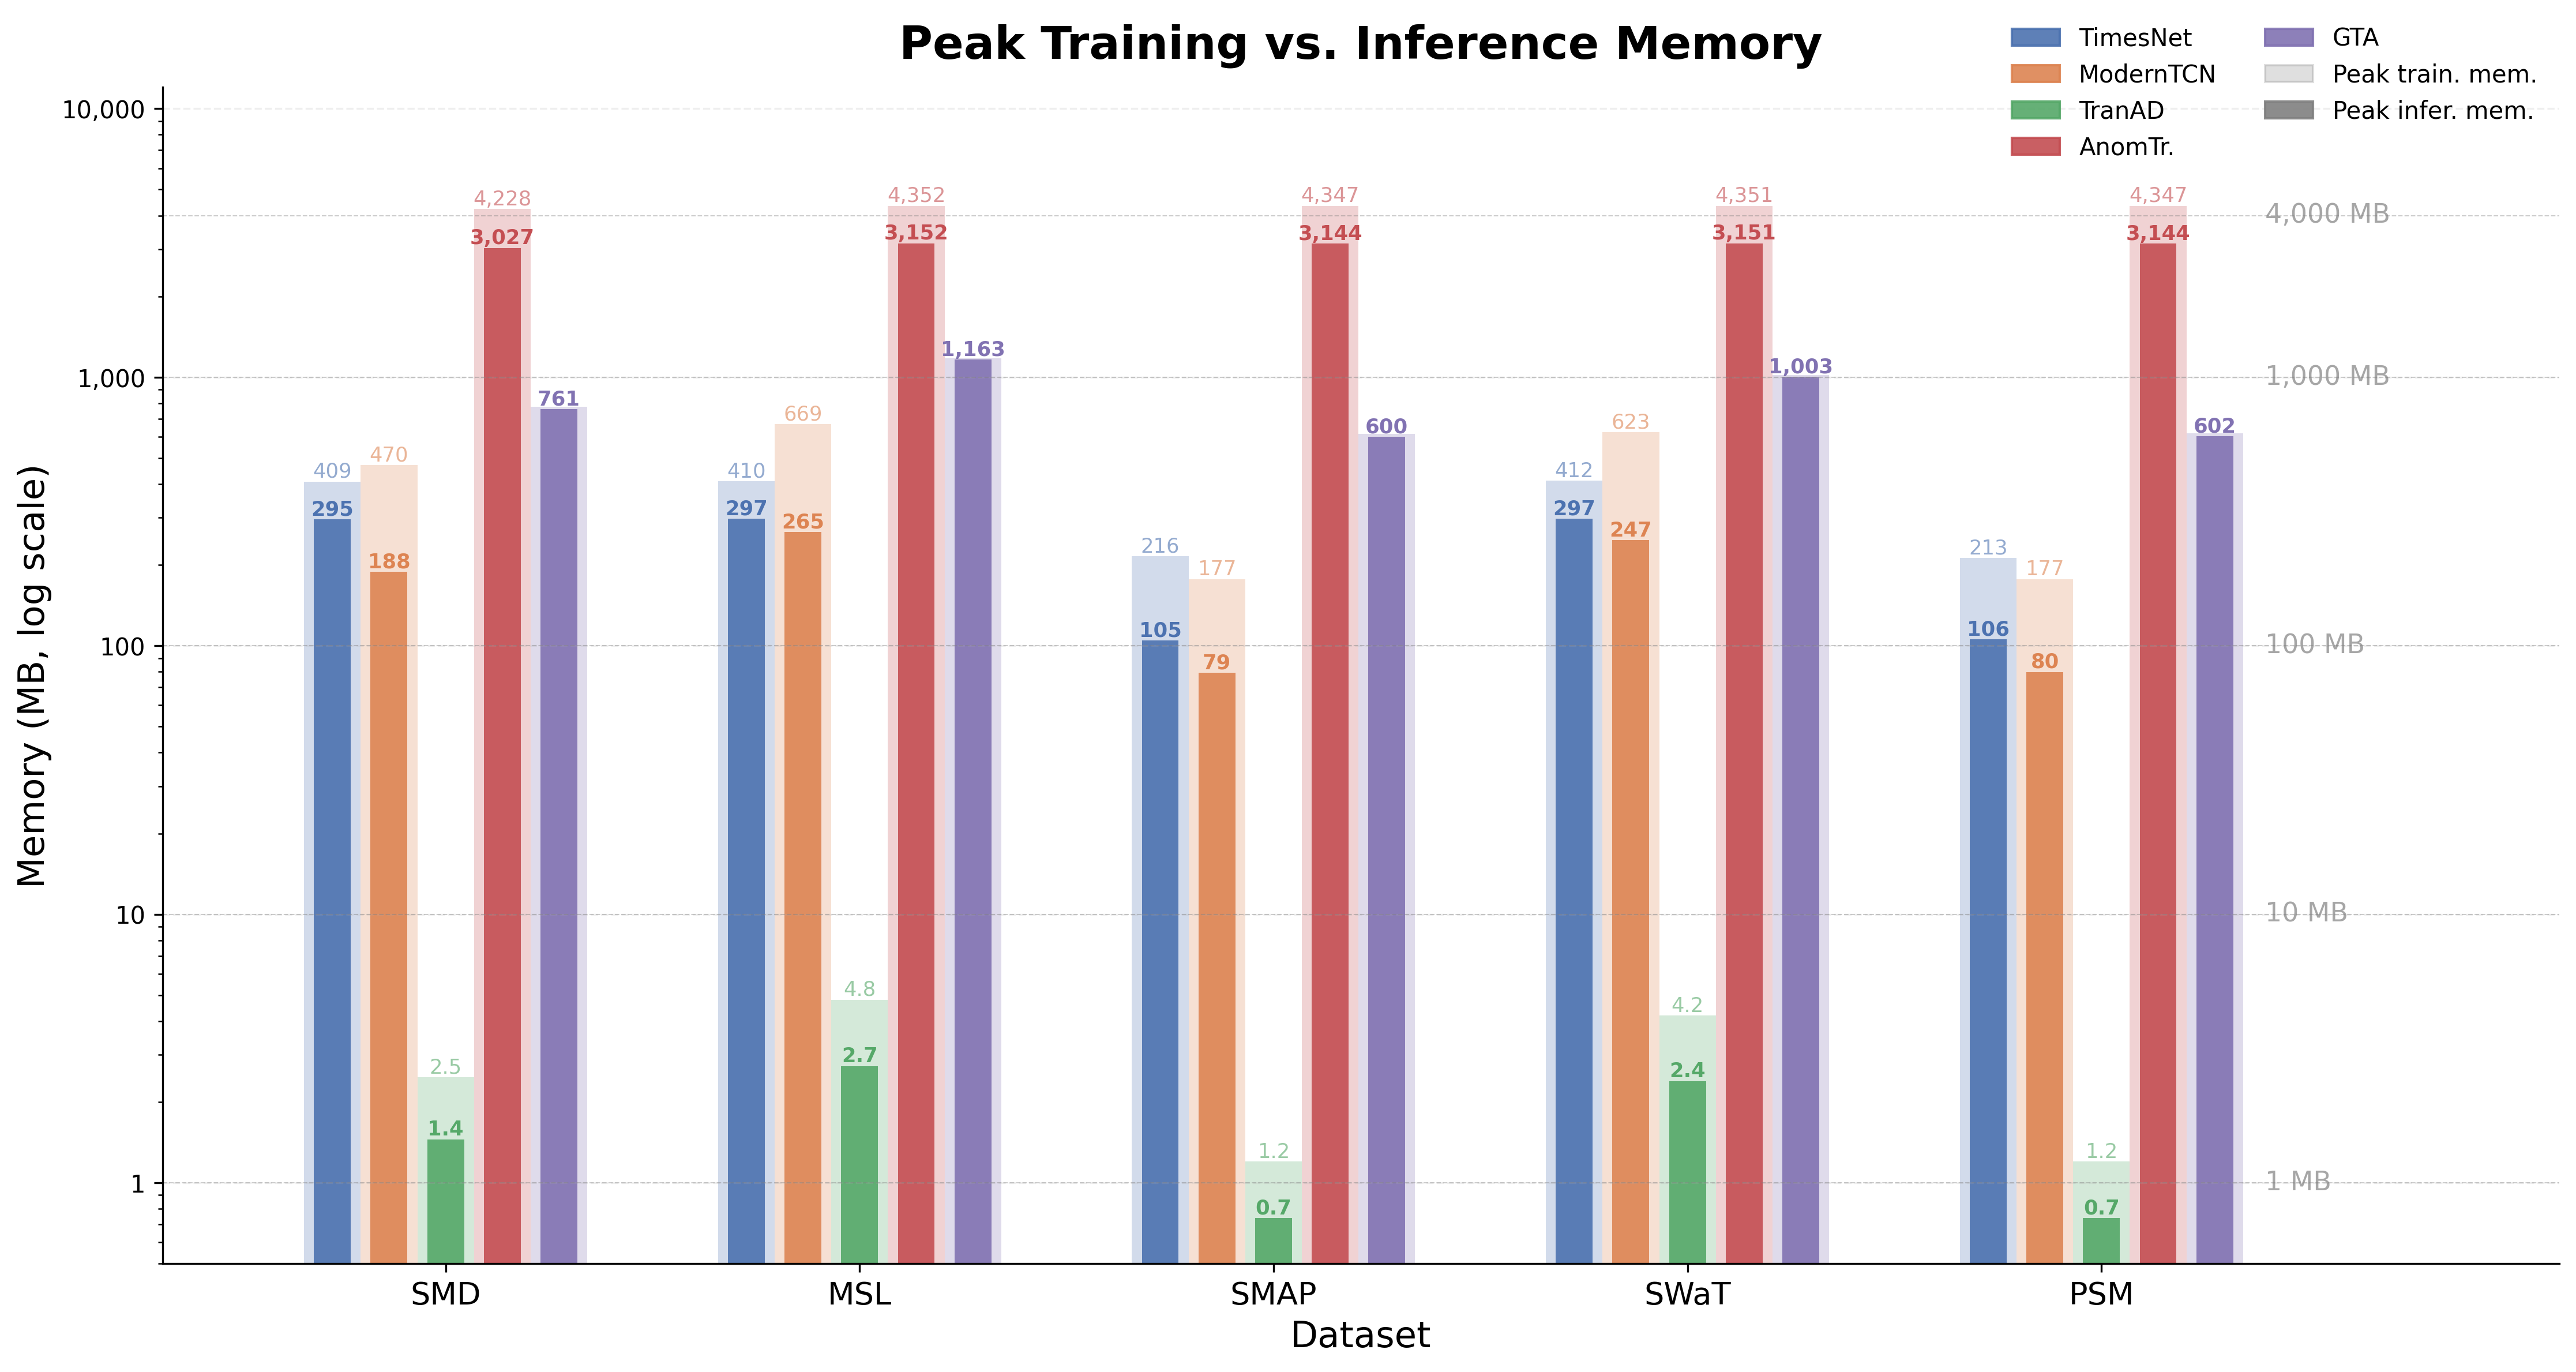
\includegraphics[width=\textwidth]{runtime_memory_logscale.png}
    \caption{Peak training and peak inference memory per model across five benchmark
    datasets (server environment), on a log scale. For each model, the faded bar
    represents peak training memory and the solid bar represents peak inference memory.
    Values shown above each bar in MB.}
    \label{fig:runtime_memory_logscale}
\end{figure}

A closer comparison of TimesNet and ModernTCN reveals an instructive divergence between
static and runtime memory behaviour. In terms of static footprint, ModernTCN is
consistently the lighter model: its average W\textsubscript{alloc} of 2.41\,MB is
roughly 9$\times$ smaller than TimesNet's 21.35\,MB, a direct consequence of its
parameter-efficient depthwise convolution design as discussed in
Section~\ref{subsubsec:static_memory}. At runtime, however, this advantage partially
inverts. On higher-dimensional datasets --- SMD, MSL, and SWaT --- ModernTCN's peak
training memory of 470.28\,MB, 669.29\,MB, and 623.31\,MB respectively exceeds
TimesNet's 408.97\,MB, 410.13\,MB, and 411.52\,MB by a substantial margin. This is
a counterintuitive result: a model with roughly 9$\times$ fewer allocated weights
produces a larger computational graph during backpropagation. 

The picture changes considerably when moving from training to inference, which is the
operationally relevant regime for edge deployment. Both models shed a large fraction
of their runtime memory when the computational graph is discarded, but ModernTCN
benefits more. On the lower-dimensional datasets SMAP and PSM, ModernTCN's inference
memory of approximately 79--80\,MB represents a reduction of roughly 55\% from its
training memory of approximately 177\,MB, while TimesNet drops from approximately
213--216\,MB to approximately 105--106\,MB, a reduction of roughly 51\%. The gap is
more pronounced on higher-dimensional datasets: on MSL, ModernTCN's inference memory
of 264.98\,MB is a 60\% reduction from its training peak of 669.29\,MB, whereas
TimesNet's inference memory of 296.63\,MB represents only a 28\% reduction from its
training peak of 410.13\,MB. The result is that at inference, ModernTCN is the
lighter of the two on every dataset despite being heavier during training on the
higher-dimensional ones, with an average inference memory of 171.93\,MB compared to
TimesNet's 219.81\,MB. For the specific context of edge deployment --- where only
inference is performed --- ModernTCN's runtime profile is therefore more favourable
than TimesNet.

GTA's runtime memory profile reveals a different pattern from what its static
footprint alone would suggest. Its average peak training memory of 841.79\,MB is
the second highest among all models after Anomaly Transformer, driven by a large
overhead of 825.86\,MB. This indicates that
GTA's computational graph retains a substantial amount of intermediate activations
during backpropagation, consistent with the deep graph convolution layers that must 
propagate gradients through the learned
adjacency structure \citep{gta2022}. At inference, however, GTA sheds a
significant fraction of this cost: its average peak inference memory of 409.75\,MB
represents a reduction of roughly 51\% from the training peak, indicating that
discarding the computational graph does yield a meaningful memory saving.

\subsubsection{Runtime Memory Footprint On Edge Device}

Memory profiling on the edge device yielded results closely matching the server
environment for four of the five models, confirming that the relative ordering and
absolute footprints established in Section~\ref{subsubsec:runtime_server} are
representative of the target deployment scenario and not an artefact of the server
hardware. The one exception was Anomaly Transformer, which triggered an
out-of-memory error on the edge device at the original batch size of 128. To obtain
valid measurements, the batch size was reduced to 64 for Anomaly Transformer on the
edge device; all other models were profiled at the original batch size.

\begin{table}[ht]
\centering
\caption{Static and runtime memory footprint of Anomaly Transformer on the edge device
(batch size = 64). All memory values in MB.}
\label{tab:memory_runtime_edge_anomtr}
\begin{tabular}{l rrrrr}
\toprule
\textbf{Metric} $\downarrow$
    & \textbf{SMD}
    & \textbf{MSL}
    & \textbf{SMAP}
    & \textbf{SWaT}
    & \textbf{PSM} \\
\midrule
Params              & 4{,}828{,}222 & 4{,}863{,}055 & 4{,}801{,}585 & 4{,}854{,}859 & 4{,}801{,}585 \\
W\textsubscript{ex} &         18.42 &         18.55 &         18.32 &         18.52 &         18.32 \\
W\textsubscript{alloc} &      28.30 &         28.43 &         28.20 &         28.40 &         28.20 \\
Peak train          &      1552.57  &      2120.92  &      2118.75  &      2122.15  &      2118.70  \\
Peak infer          &      1484.07  &      1548.87  &      1543.49  &      1548.75  &      1543.49  \\
OH                  &      1524.27  &      2092.49  &      2090.55  &      2093.74  &      2090.50  \\
\bottomrule
\end{tabular}
\end{table}

Even at the reduced batch size, Anomaly Transformer's runtime memory footprint
remains substantial, as shown in Table~\ref{tab:memory_runtime_edge_anomtr}. 
Peak training memory ranges from 1552.57\,MB on SMD to
2122.15\,MB on SWaT, and peak inference memory from 1484.07\,MB on SMD to
1548.87\,MB on MSL --- figures that are roughly half of those observed on the
server at batch size 128, consistent with the linear scaling of activation memory
with batch size. Critically, however, these reduced figures still represent 
the highest runtime memory demand of any
model evaluated in this thesis, and were only obtainable by halving the batch size. 
The out-of-memory error at
batch size 128 is itself a meaningful result: it demonstrates that Anomaly
Transformer cannot be operated under standard training conditions on this class of
hardware.


\subsection{Inference Speed and Number of Operations}

For IoT edge deployment, inference speed and arithmetic cost are complementary
constraints: a model must both complete each forward pass within the response-time
budget of the target application \emph{and} do so with a computational workload
that the available floating-point hardware can sustain continuously without
accumulating a processing backlog. The two metrics introduced
in Section~\ref{sec:eval_metrics} --- Inference Speed and Number of Operations --- 
capture these
constraints from different angles. MAC count is a hardware-independent measure of
computational complexity that allows cross-model comparison regardless of execution
environment, while wall-clock latency reflects the end-to-end delay experienced on
a specific platform and is therefore the operationally decisive figure for deployment.

As established in Section~\ref{subsec:memory},
TranAD \citep{tranad2022} hardcodes execution to the CPU via explicit
\texttt{.cpu()} calls, meaning it never utilises a GPU even when one is available.
One might expect this to result in severely degraded latency relative to
GPU-accelerated models; the measured results tell a more nuanced story.
This illustrates that neither MAC count nor hardware execution context alone is
sufficient to predict on-device performance, and that architecture-level
properties --- such as model depth and sequence length --- interact with the
execution environment in non-obvious ways.

Measurements were conducted in the same two hardware environments used for memory
profiling. The server environment provides a GPU-accelerated baseline representative
of standard development conditions, while the edge device measurements surface the
latency penalties that arise when models designed for server hardware are transferred
to constrained embedded platforms. The remainder of this section presents MAC counts
and latency figures for all evaluated models, followed by a discussion of their
implications for edge deployment.

\subsubsection{Number of Operations}
\label{subsubsec:mac_results}

All MAC counts are measured using \texttt{fvcore} \citep{fvcore}, as described in
Section~\ref{subsec:macs}. For the CNN-based models --- TimesNet
\citep{timesnet2023} and ModernTCN \citep{moderntcn2024} --- the built-in handlers
provided sufficient coverage, since their dominant cost lies in convolutional and
linear layers that \texttt{fvcore} handles natively. For the Transformer-based
models --- TranAD \citep{tranad2022}, Anomaly Transformer
\citep{anomalytransformer2022}, and GTA \citep{gta2022} --- custom operator handlers
were implemented and registered to cover operations silently omitted by default,
for instance element-wise arithmetic (\texttt{aten::mul}). For
Anomaly Transformer, the Gaussian kernel computation used to derive the
prior-association is entirely invisible to \texttt{fvcore} and was therefore
computed analytically and added manually to the reported total. All MAC counts
should consequently be interpreted as lower bounds on the true per-forward-pass
cost, suitable for relative cross-model comparison rather than absolute throughput
estimation.

\begin{table}[ht]
\centering
\caption{MAC count per forward pass per model across five benchmark datasets.
All values in kilo-MACs (kMACs). Lowest value per column in \textbf{bold}, second-lowest
\underline{underlined}.}
\label{tab:mac_counts}
\begin{tabular}{l rrrrr r}
\toprule
\textbf{Dataset}
    & \thead{\textbf{TimesNet}\\\citep{timesnet2023}}
    & \thead{\textbf{ModernTCN}\\\citep{moderntcn2024}}
    & \thead{\textbf{TranAD}\\\citep{tranad2022}}
    & \thead{\textbf{AnomTr.}\\\citep{anomalytransformer2022}}
    & \thead{\textbf{GTA}\\\citep{gta2022}} \\
\midrule
SMD  & 2{,}123{,}747 & \underline{17{,}145} & \textbf{894}   & 515{,}923 & 30{,}986 \\
MSL  & 2{,}110{,}124 & \underline{27{,}808} & \textbf{1{,}791} & 519{,}407 & 34{,}220 \\
SMAP &   589{,}610   &  \underline{3{,}840} & \textbf{415}   & 513{,}260 & 29{,}099 \\
SWaT & 2{,}138{,}137 & \underline{25{,}132} & \textbf{1{,}552} & 518{,}587 & 33{,}381 \\
PSM  &   583{,}753   &  \underline{3{,}840} & \textbf{415}   & 513{,}260 & 29{,}099 \\
\midrule
Avg  & 1{,}509{,}074 & \underline{15{,}553} & \textbf{1{,}013} & 516{,}087 & 31{,}357 \\
\bottomrule
\end{tabular}
\end{table}

The MAC counts in Table~\ref{tab:mac_counts} reveal a ranking that closely mirrors
the static memory footprint results of Section~\ref{subsubsec:static_memory}.

TranAD \citep{tranad2022} is by far the most computationally efficient model,
with an average of just 1{,}013 kMACs per forward pass --- more than an order
of magnitude fewer than any other model. This is a direct consequence of its compact
architecture: with an average of 145{,}769 parameters across datasets, TranAD performs
only the minimum computation necessary to reconstruct the input window through its
shallow encoder-decoder structure \citep{tranad2022}. It should be noted that
TranAD's two inference phases are both captured in this figure, as Phase~2 depends
on the output of Phase~1 and the two execute sequentially within a single forward
pass \citep{tranad2022}. The reported MAC count therefore reflects the full
computational cost of one inference step.

TimesNet \citep{timesnet2023} exhibits the widest spread of MAC counts across
datasets, ranging from 583{,}753 kMACs on PSM and SMAP to over 2{,}1M kMACs on SMD, MSL,
and SWaT. As established in Section~\ref{subsubsec:static_memory}, this variability
is a direct consequence of TimesNet's input-adaptive hidden dimension $d_\text{model}$,
which scales with the number of input features (Equation~\ref{eq:timesnet_dmodel}).
Since most weight matrices scale quadratically with $d_\text{model}$, the number of
operations follows the same two-cluster pattern as the parameter count: datasets with
higher-dimensional inputs incur substantially more computation per forward pass.

ModernTCN \citep{moderntcn2024} exhibits the same input-adaptive scaling behaviour,
producing an identical two-cluster pattern across datasets. However, its use of
depthwise and grouped pointwise convolutions rather than dense 2D inception blocks
translates into substantially lower MAC counts at every dataset, averaging
15{,}553 kMACs compared to TimesNet's 1{,}509{,}074 --- a reduction of
roughly two orders of magnitude. ModernTCN is therefore the most computationally
efficient CNN-based model evaluated in this thesis by a wide margin.

Anomaly Transformer \citep{anomalytransformer2022} produces high but remarkably
consistent MAC counts across datasets, averaging 516{,}087 kMACs with negligible
variation. This mirrors its near-constant static memory footprint and stems from the
same architectural property: its fixed hidden dimension of $d_\text{model} = 512$
means that the dominant cost --- the attention computation over
the sequence length $N$ --- is entirely independent of input dimensionality
\citep{anomalytransformer2022}.

GTA \citep{gta2022} occupies a moderate, stable position in the ranking, averaging
31{,}357 kMACs with little variation across datasets. This places it well below
Anomaly Transformer and TimesNet, but above TranAD and ModernTCN.
The relative consistency of GTA's MAC count reflects the fact that its dominant
computational cost --- the graph convolution and dilated convolution layers
--- scales primarily with sequence length rather than input dimensionality
\citep{gta2022}.

\subsubsection{Inference Speed}
\label{subsubsec:latency_results}

Latency and throughput are measured across the same two hardware environments used
for memory and MAC profiling. Latency is reported as the mean wall-clock time per
batch in milliseconds, captured using \texttt{time.perf\_counter()} for CPU-resident
models and CUDA Events for GPU-accelerated models. Throughput is derived as the number of 
individual input windows processed per second.
Both metrics are averaged over
multiple inference runs on the test set to reduce timing variance. As noted in
Section~\ref{subsubsec:mac_results}, MAC count alone does not predict wall-clock
latency: hardware execution context and architectural properties interact in ways that
make the two measures complementary rather than redundant, and the results below
illustrate this concretely.

\begin{table}[ht]
\centering
\caption{Mean batch latency (ms) and throughput (input windows/s) per model across five
benchmark datasets. Lowest latency per column in \textbf{bold}, second-lowest
\underline{underlined}. Highest throughput per column in \textbf{bold},
second-highest \underline{underlined}.}
\label{tab:latency}
\begin{tabular}{ll rrrrr r}
\toprule
& \textbf{Dataset}
    & \thead{\textbf{TimesNet}\\\citep{timesnet2023}}
    & \thead{\textbf{ModernTCN}\\\citep{moderntcn2024}}
    & \thead{\textbf{TranAD}\\\citep{tranad2022}}
    & \thead{\textbf{AnomTr.}\\\citep{anomalytransformer2022}}
    & \thead{\textbf{GTA}\\\citep{gta2022}} \\
\midrule
\multirow{5}{*}{\rotatebox[origin=c]{90}{\textbf{Latency}}}
& SMD  & 140.2 & \textbf{6.6}  & \underline{10.2} & 33.0 & 63.2 \\
& MSL  & 145.0 & \textbf{8.8}  & \underline{16.1} & 33.4 & 69.3 \\
& SMAP &  42.4 & \underline{12.4} & \textbf{8.2}  & 33.5 & 59.3 \\
& SWaT & 151.3 & \textbf{8.2}  & \underline{11.8} & 34.2 & 68.3 \\
& PSM  &  54.0 & \underline{12.4} & \textbf{8.3}  & 34.5 & 59.7 \\
& Avg  & 106.6 & \textbf{9.7}  & \underline{10.9} & 33.7 & 64.0 \\
\midrule
\multirow{5}{*}{\rotatebox[origin=c]{90}{\textbf{Throughput}}}
& SMD  &   913 & \textbf{19{,}482} & \underline{12{,}598} & 3{,}882 & 2024 \\
& MSL  &   883 & \textbf{14{,}525} & \underline{7{,}935}  & 3{,}833 & 1848 \\
& SMAP & 3022 & \underline{10{,}342} & \textbf{15{,}519} & 3{,}820 & 2158 \\
& SWaT &   846 & \textbf{15{,}545} & \underline{10{,}837} & 3{,}742 & 1874 \\
& PSM  & 2370 & \underline{10{,}341} & \textbf{10{,}837} & 3{,}708 & 2144 \\
& Avg  & 1607 & \textbf{14{,}047} & \underline{11{,}545} & 3{,}797 & 2009 \\
\bottomrule
\end{tabular}
\end{table}

The latency and throughput results in Table~\ref{tab:latency} reveal a ranking that
diverges from the MAC count ordering, illustrating that operation count
alone is insufficient to predict wall-clock inference time.

ModernTCN \citep{moderntcn2024} achieves the lowest average latency of 9.7\,ms and
the highest average throughput of 14{,}047 input windows per second, consistent with its
low MAC count and GPU-accelerated execution. This result is expected: few operations
combined with hardware parallelism translate directly into fast inference.

Despite sharing a convolutional backbone with ModernTCN, TimesNet
\citep{timesnet2023} is by far the slowest model, with an average latency of
106.6\,ms, more than ten times higher than ModernTCN. The additional latency 
overhead stems from
TimesNet's architectural design: unlike ModernTCN, which operates directly on 1D
time series via depthwise and grouped convolutions, TimesNet transforms the input
into 2D space to leverage 2D convolutional backbones from the computer vision
community. As noted by the authors of ModernTCN \citep{moderntcn2024}, this additional 
data transformation
and aggregation step introduces memory overhead and slower execution speed. 
TimesNet also exhibits the same
two-cluster latency pattern seen in its MAC and memory results: latency on
higher-dimensional datasets (SMD, MSL, SWaT) is roughly three times higher than
on lower-dimensional ones (SMAP, PSM), directly reflecting the input-adaptive
scaling of $d_\text{model}$.

The most striking result is TranAD \citep{tranad2022}, which achieves the second
lowest average latency of 10.9\,ms despite executing entirely on the CPU. One might
expect CPU execution to impose a severe latency penalty relative to GPU-accelerated
models; the results show otherwise. TranAD's architectural simplicity --- its shallow
encoder-decoder with an average of just 1{,}013 kMACs per forward pass ---
more than compensates for the absence of GPU parallelism. On SMAP and PSM,
TranAD even surpasses ModernTCN in both latency and throughput.

Anomaly Transformer \citep{anomalytransformer2022} achieves consistent latency of
approximately 33--34\,ms across all datasets, mirroring the near-constant MAC count
observed in Section~\ref{subsubsec:mac_results}. Its fixed $d_\text{model} = 512$
makes inference time effectively independent of input dimensionality, resulting in
predictable but moderate performance that places it third in the ranking.

GTA \citep{gta2022} is the second slowest model. Its average latency of 64.0\,ms suggests
that GTA incurs runtime overhead beyond raw arithmetic cost, likely from the
graph construction and adjacency matrix operations.

\subsubsection{Inference Speed on Edge Device}
Table~\ref{tab:latency_edge} reports latency and throughput measured directly on the
edge device. The experimental setup mirrors the server environment, with one
exception: as noted in Section~\ref{subsubsec:runtime_server}, Anomaly Transformer
triggered an out-of-memory error on the edge device at the original batch size of
128, and was therefore profiled at a reduced batch size of 64.
This reduction affects the absolute throughput figure for Anomaly Transformer (a smaller 
batch processes fewer samples per forward pass) and also affects latency, since latency 
depends on the batch size. However, results are still reported in this configuration due 
to memory constraints, and latency is interpreted as model inference time under the maximum 
feasible batch size for each model.

\begin{table}[ht]
\centering
\caption{Mean batch latency (ms) and throughput (input windows/s) per model across five
benchmark datasets on the edge device. Lowest latency per column in \textbf{bold},
second-lowest \underline{underlined}. Highest throughput per column in \textbf{bold},
second-highest \underline{underlined}. AnomTr.\ profiled at batch size 64;
all other models at batch size 128.}
\label{tab:latency_edge}
\begin{tabular}{ll rrrrr r}
\toprule
& \textbf{Dataset}
    & \thead{\textbf{TimesNet}\\\citep{timesnet2023}}
    & \thead{\textbf{ModernTCN}\\\citep{moderntcn2024}}
    & \thead{\textbf{TranAD}\\\citep{tranad2022}}
    & \thead{\textbf{AnomTr.}\\\citep{anomalytransformer2022}}
    & \thead{\textbf{GTA}\\\citep{gta2022}} \\
\midrule
\multirow{6}{*}{\rotatebox[origin=c]{90}{\textbf{Latency}}}
& SMD  & 398.8 & \textbf{66.4}  & \underline{103.4}  & 138.9 & 887.8 \\
& MSL  & 399.0 & \textbf{95.1}  & \underline{137.5} & 138.9 & 974.5 \\
& SMAP & 252.8 & \textbf{21.5}  & \underline{79.8}  & 138.4 & 792.2 \\
& SWaT & 398.4 & \textbf{88.2}  & \underline{137.0} & 138.9 & 955.5 \\
& PSM  & 253.0 & \textbf{21.5}  & \underline{81.1}  & 138.4 & 791.8 \\
& Avg  & 340.4 & \textbf{58.6}  & \underline{107.8} & 138.7 & 880.3 \\
\midrule
\multirow{6}{*}{\rotatebox[origin=c]{90}{\textbf{Throughput}}}
& SMD  &   321 & \textbf{1{,}927} & \underline{1{,}238} &   461 &  144 \\
& MSL  &   321 & \textbf{1{,}346} & \underline{930}     &   461 &  131 \\
& SMAP &   507 & \textbf{5{,}943} & \underline{1{,}604} &   462 &  162 \\
& SWaT &   321 & \textbf{1{,}452} & \underline{934}     &   461 &  134 \\
& PSM  &   506 & \textbf{5{,}941} & \underline{1{,}578} &   463 &  162 \\
& Avg  &   395 & \textbf{3{,}327} & \underline{1{,}257} &   461 &  147 \\
\bottomrule
\end{tabular}
\end{table}

Figure~\ref{fig:latency_scatter} plots average latency against average throughput
for both environments, making the cross-environment shift in rankings immediately
visible. On the server, TranAD and ModernTCN occupy the same high-throughput,
low-latency corner of the plot, with TranAD at 10.9\,ms and ModernTCN at 9.7\,ms
--- a negligible difference that suggests CPU execution imposes little penalty when
the model is sufficiently lightweight. On the edge device, this picture changes
considerably: ModernTCN retains its position as the fastest model at 58.6\,ms,
while TranAD falls back to 107.8\,ms, nearly doubling its latency. The gap between
the two widens from under 2\,ms on the server to approximately 49\,ms on the edge,
indicating that the absence of GPU acceleration becomes more consequential on
constrained hardware where CPU performance is also more limited.

\begin{figure}[ht]
    \centering
    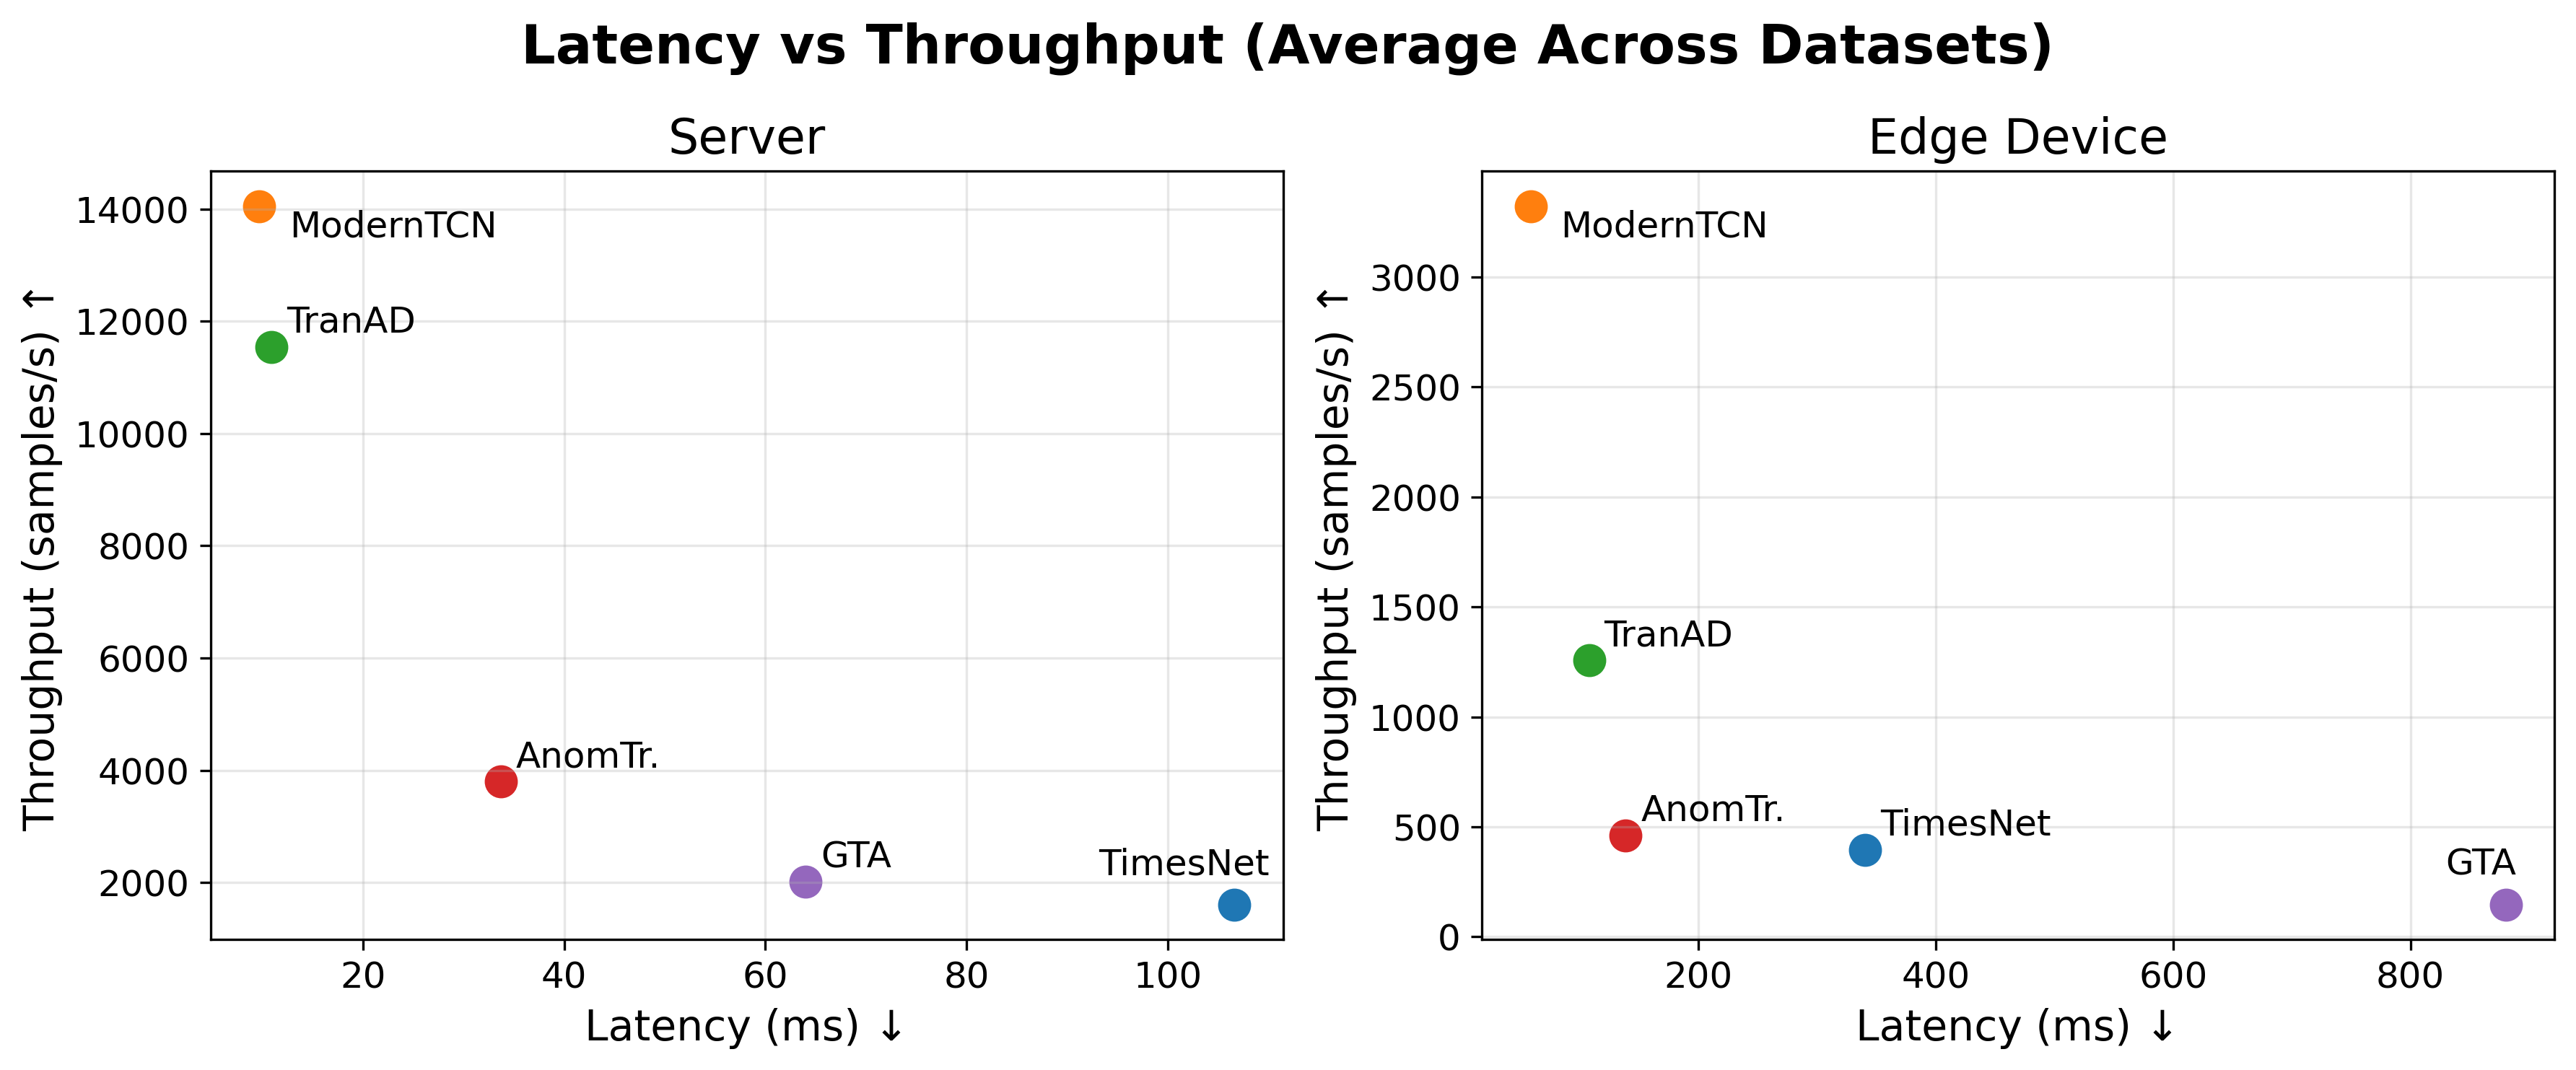
\includegraphics[width=\textwidth]{latency_throughput.png}
    \caption{Average latency (ms) versus throughput (input windows/s) for all five models
    on the server (left) and edge device (right). The ideal region is the top-left
    corner (low latency, high throughput). }
    \label{fig:latency_scatter}
\end{figure}

GTA \citep{gta2022} stands out as a clear outlier on the edge device, where its 
average latency of 880.3\,ms places it
far to the right of all other models. Even on the server, where it achieves
64.0\,ms, GTA is the second slowest model despite having a moderate MAC count ---
a pattern attributed in Section~\ref{subsubsec:mac_results} to runtime overhead
from its graph construction and adjacency matrix operations. On the edge device
this overhead compounds further, resulting in a slowdown factor of approximately
13.8$\times$, the largest of any model evaluated. TimesNet \citep{timesnet2023},
by contrast, degrades more gracefully: despite being the slowest model on the
server at 106.6\,ms, its edge latency of 340.4\,ms represents a slowdown of
roughly 3.2$\times$, the smallest of all five models.

\begin{figure}[ht]
    \centering
    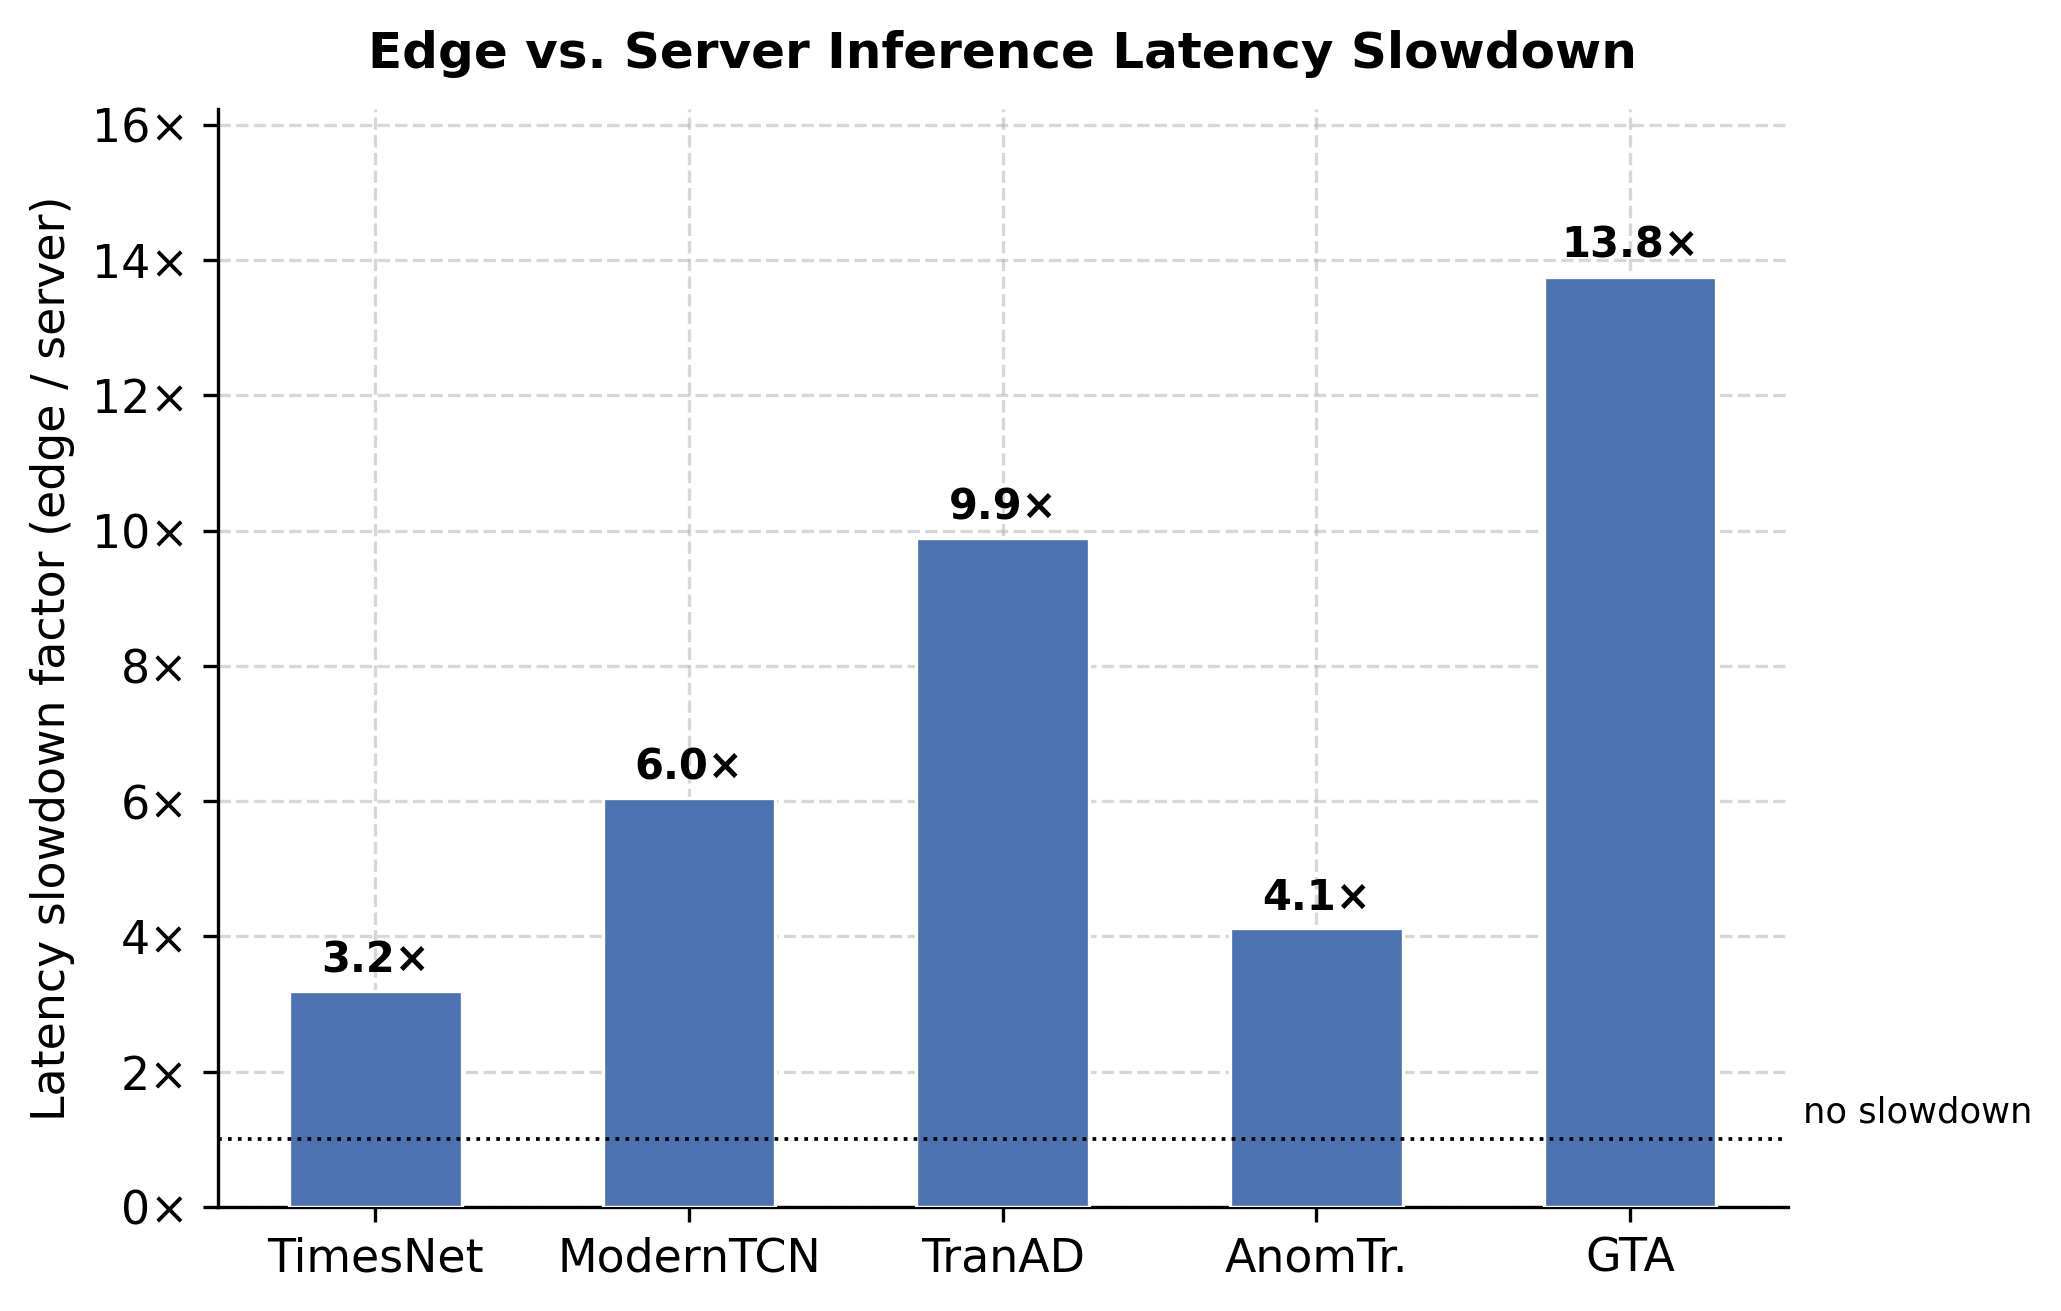
\includegraphics[width=0.85\textwidth]{latency_slowdown.png}
    \caption{Latency increase factor (edge / server) for each model, computed as
    the ratio of average edge latency to average server latency. The dotted line
    at 1$\times$ marks the baseline of no slowdown. TranAD executes on CPU in
    both environments; all other models execute on GPU.}
    \label{fig:latency_slowdown}
\end{figure}

Figure~\ref{fig:latency_slowdown} shows the latency increase factor for each model
when moving from the server to the edge device. All models are slower on the edge,
as expected, but the degree of degradation varies substantially across architectures
and does not follow the MAC count ranking.

TimesNet \citep{timesnet2023} degrades the least, with a increase factor of only
3.2$\times$. This is the smallest penalty of any model despite TimesNet being the
slowest model in absolute terms on both platforms. The result suggests that
TimesNet's 2D convolutional operations, while computationally expensive, translate
relatively efficiently to the edge hardware.

Anomaly Transformer \citep{anomalytransformer2022} follows with a a latency 
increase factor of
4.1$\times$, the second most graceful degradation. Its fixed architecture and
consistent MAC count across datasets appear to result in predictable and moderate
scaling behaviour across hardware environments. (On the server environment, Anomaly 
Transformer was evaluated using the standard batch size of 128, while on the edge 
device it was executed at a reduced batch size due to memory constraints, and the 
reported latency increase reflects this deployment setting.)

ModernTCN \citep{moderntcn2024} incurs a 6.0$\times$ latency increase. While it remains
the fastest model in absolute latency on both platforms, the penalty is larger than
one might expect for a lightweight convolutional model, suggesting that some of its
efficiency advantage on the server is tied to GPU parallelism that is less available
on the edge device.

TranAD \citep{tranad2022} shows a 9.9$\times$ latency increase --- the second largest ---
which is particularly notable given that it already runs on the CPU on the server.
The result indicates that the edge device's CPU is substantially less capable than
the server CPU, amplifying the cost of CPU-only execution in a constrained
environment.

GTA \citep{gta2022} exhibits by far the largest latency increase at 13.8$\times$,
confirming that its persistent graph construction overhead does not scale well to
constrained hardware. Combined with its already high absolute latency on the server,
this makes GTA the least suitable model for edge deployment among those evaluated.


%%%%%%%%%%%%%%%%%%%%%%%%%%%%%%%%%%%%%%%%%%%%%%%%%%%%%%%%%%%%%%%%%%%%%%%

\chapter{Conclusion}
\label{ch:conclusion}

This thesis investigated the suitability of five deep learning models for
time series anomaly detection in IoT edge deployment scenarios, evaluated
along two complementary axes: detection accuracy and computational efficiency.
The five models --- TimesNet \citep{timesnet2023}, ModernTCN \citep{moderntcn2024},
TranAD \citep{tranad2022}, Anomaly Transformer \citep{anomalytransformer2022},
and GTA \citep{gta2022} --- were selected to represent a diverse range of
architectures spanning convolutional, transformer-based, and graph-based
approaches. Each model was trained and evaluated on five widely adopted benchmark
datasets --- SMD, MSL, SMAP, SWaT, and PSM --- following the experimental
setup described in each model's original publication. Detection accuracy was
assessed using point-adjusted F1 score and AU-PR, while efficiency was
characterised through MAC counts, memory footprint, and inference speed,
measured on both a server-grade GPU environment and a resource-constrained
edge device.

\section{Evaluation Summary}
Figure~\ref{fig:parallel_coords} presents a parallel coordinates plot summarising
the performance of all five models across six evaluation dimensions: F1 score,
peak training memory, peak inference memory, inference latency, throughput, and
MAC count. All efficiency values --- training memory, inference memory, latency,
and throughput --- are taken from the edge device experiments, making this a
direct assessment of each model's suitability for the target deployment scenario.
The values shown represent averages across all five benchmark datasets.
To enable visual comparison across metrics with fundamentally different
units and scales, all values are normalised to the range $[0, 1]$ using the
observed minimum and maximum across the five models as the range boundaries: a
value equal to the best observed result maps to 1, and a value equal to the worst
observed result maps to 0. For metrics where a lower value is better --- training
memory, inference memory, latency, and kMACs --- the normalised values are
subsequently inverted so that a higher position on every axis consistently
indicates better performance. Throughput, like F1, is higher-is-better and
requires no inversion.

\begin{figure}[ht]
    \centering
    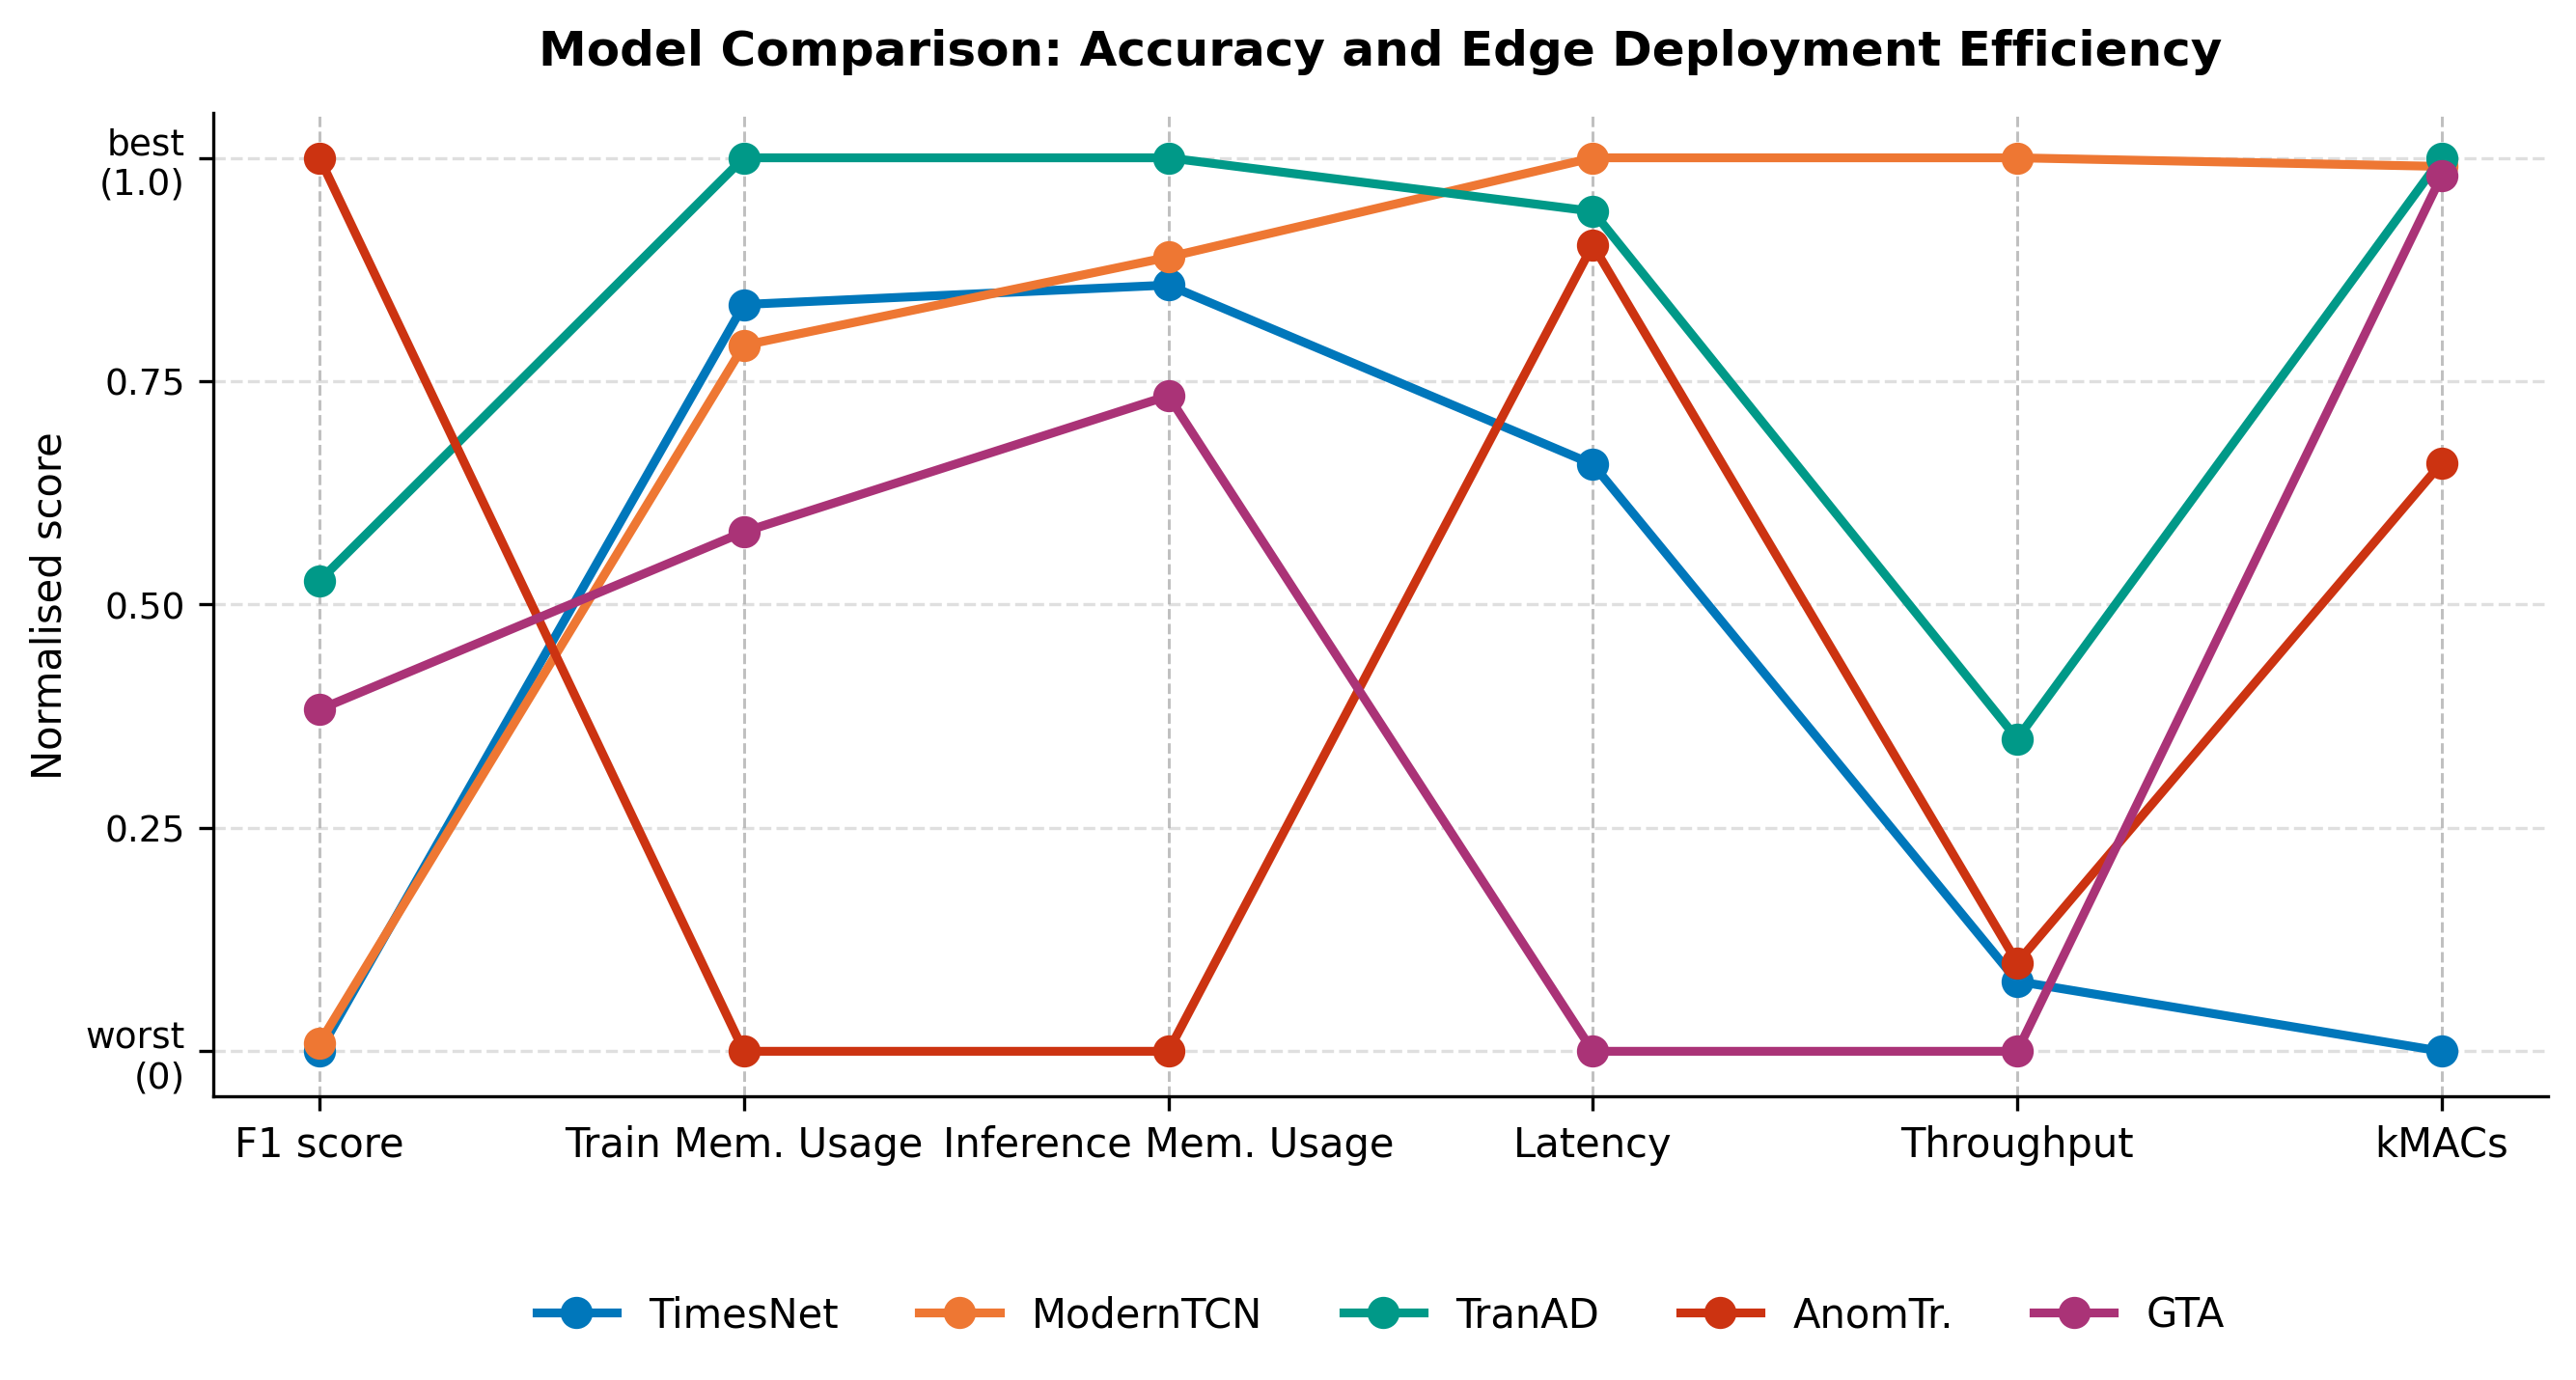
\includegraphics[width=\textwidth]{parallel_coords.png}
    \caption{Parallel coordinates plot comparing all five models across six
    evaluation metrics, averaged across the five benchmark datasets.
    All axes are normalised to $[0, 1]$ where 1 = best. For metrics where
    a lower value is preferable --- training memory, inference memory,
    latency, and kMACs --- the normalised scores are inverted, so that a
    model with lower raw values appears higher on the axis. Throughput and
    F1 require no inversion as higher raw values are already better.}
    \label{fig:parallel_coords}
\end{figure}

The plot reveals a trade-off between detection accuracy and deployment
efficiency that runs through the entire model comparison. Anomaly Transformer
\citep{anomalytransformer2022} achieves the highest normalised F1 score but
collapses to zero on both memory axes, reflecting its prohibitive runtime memory
demand documented in Section~\ref{subsubsec:runtime_server}. Despite its leading
accuracy, this makes it the least suitable model for resource-constrained edge
deployment. 

At the opposite end of the spectrum, TranAD \citep{tranad2022} and ModernTCN
\citep{moderntcn2024} emerge as the two strongest candidates for edge deployment,
and the choice between them is not straightforward. Both achieve competitive F1
scores and low kMAC counts, meaning these two metrics alone do not differentiate
them meaningfully. The distinction lies in the remaining efficiency dimensions.
TranAD excels on memory: it has by far the lowest training and inference memory
footprint of any model, and achieves good latency despite running entirely on the
CPU. On the other hand, its throughput is weaker than ModernTCN. 
ModernTCN, by contrast, is the strongest model on latency
and throughput, and maintains a consistent profile across all metrics without any
notable weakness, though it requires considerably more memory than TranAD.

The choice between the two therefore depends on the specific constraints of the
target deployment. If memory efficiency is the primary concern --- for instance on
devices with very limited RAM budgets --- TranAD is the better choice, as its
memory footprint is in a category of its own. If latency and throughput are the
binding constraints --- for instance in applications that must process high-rate
sensor streams in real time --- ModernTCN is the more suitable option.

GTA \citep{gta2022} and TimesNet \citep{timesnet2023} present the weakest overall
profiles. GTA has the worst latency of all five models without compensating with a
particularly strong F1 or memory advantage. TimesNet has the highest computational
cost by a large margin, reflecting its expensive 2D data transformation, and
achieves the lowest F1 of all five models. Neither model offers a compelling case
for edge deployment relative to the alternatives evaluated here.

Taken together, analyzing the results supports two conclusions. First, no
single model dominates on all metrics simultaneously, confirming that accuracy and
efficiency represent genuinely competing objectives in this benchmark. Second, the
choice of model depends on the deployment context: if memory is the
binding constraints, TranAD is the recommended choice; if a balance across all
dimensions is required, ModernTCN is the strongest all-rounder. Anomaly
Transformer, despite its accuracy leadership, is not a viable candidate for
resource-constrained IoT edge deployment under the conditions evaluated in this
thesis.

\section{Future work}

Several directions emerge naturally from the findings of this thesis.

The efficiency analysis reveals that Anomaly Transformer and GTA are the two
models that most clearly cannot meet the memory and compute constraints of
resource-constrained edge devices under their current implementations. A natural
next step is to investigate whether model compression techniques can close this
gap without sacrificing detection quality. Quantisation --- reducing the numerical
precision of weights and activations to
lower-bit representations --- could substantially reduce both the memory footprint
and inference cost of these models \citep{cheng2023compression}. 
Structured pruning, which removes entire attention heads, convolutional
filters, or other components that contribute little to the output, offers a
complementary route to reducing both parameter count and MAC cost \citep{cheng2023compression}. 
Knowledge distillation --- training a smaller student model to replicate the
behaviour of a larger teacher --- could in principle
produce more compact models that retain the detection quality of their larger
counterparts \citep{hinton2015distilling}. Investigating whether any of these 
approaches can preserve the detection quality
of these models under meaningful compression ratios would be a natural
extension of this work.

A second direction concerns the breadth of the evaluation. The five benchmark
datasets used in this thesis --- SMD, MSL, SMAP, SWaT, and PSM --- are widely
adopted in the TSAD literature but do not cover the full diversity of IoT
deployment scenarios. Evaluating the models on additional IoT-specific datasets,
particularly those with higher sensor counts, more complex inter-sensor
dependencies, or higher anomaly rates, would provide a more complete picture of
where each model's strengths and weaknesses manifest.

%%%%%%%%%%%%%%%%%%%%%%%%%%%%%%%%%%%%%%%%%%%%%%%%%%%%%%%%%%%%%%%%%%%%%%%

\cleardoublepage
\addcontentsline{toc}{chapter}{Bibliography}
\bibliographystyle{plain} 
\bibliography{refs}

%%%%%%%%%%%%%%%%%%%%%%%%%%%%%%%%%%%%%%%%%%%%%%%%%%%%%%%%%%%%%%%%%%%%%%%

%\cleardoublepage
%\appendix
%\chapter{The Technical Details}

%\todo{\dots}

\end{document}

